\documentclass[a4paper,12pt, PhD]{stb-thesis}

% Page layout
\usepackage[left=3cm,right=2cm,top=2.5cm,bottom=2.5cm]{geometry}
%\usepackage{cite}
\usepackage{afterpage}
\newcommand\blankpage{%
	\null
	\thispagestyle{empty}%
	\addtocounter{page}{-1}%
	\newpage}

% Subsections
\setcounter{secnumdepth}{3}
\setcounter{tocdepth}{3}

% Figures
\usepackage[margin=\the\parindent,small,bf,rm]{caption}
\usepackage{graphicx}
\usepackage{pdfpages}
\setlength{\abovecaptionskip}{8pt}  % spacing above and below captions
\usepackage{subfig}

% Font and text
\usepackage[english,afrikaans]{babel}
\usepackage{microtype}
\usepackage{setspace}
\newcommand{\myemph}[1]{{\sffamily\bfseries#1}}
\sloppy
\onehalfspacing
\usepackage{enumitem}
%\setlist[enumerate]{noitemsep, topsep=0pt, partopsep=0pt}
\usepackage{listings,xfp}
\usepackage{anyfontsize}
\usepackage{bold-extra}
\usepackage{quotchap}

\renewcommand\labelitemi{\tinytonormal$\divideontimes$}

\makeatletter
{\large % Capture font definitions of \small
	\xdef\f@size@large{\f@size}
	\xdef\f@baselineskip@large{\f@baselineskip}
	\Large % Capture font definitions for \normalsize
	\xdef\f@size@Large{\f@size}
	\xdef\f@baselineskip@Large{\f@baselineskip}
}
% Define new \smalltonormalsize font size
\newcommand{\largetoLarge}{%
	\fontsize
	{\fpeval{(\f@size@large+\f@size@Large)/2}}
	{\fpeval{(\f@baselineskip@large+\f@baselineskip@Large)/2}}%
	\selectfont
}
\makeatother
\makeatletter
{\tiny % Capture font definitions of \small
	\xdef\f@size@tiny{\f@size}
	\xdef\f@baselineskip@tiny{\f@baselineskip}
	\normalsize % Capture font definitions for \normalsize
	\xdef\f@size@normalsize{\f@size}
	\xdef\f@baselineskip@normalsize{\f@baselineskip}
}
% Define new \smalltonormalsize font size
\newcommand{\tinytonormal}{%
	\fontsize
	{\fpeval{(\f@size@tiny+\f@size@normalsize)/2}}
	{\fpeval{(\f@baselineskip@tiny+\f@baselineskip@normalsize)/2}}%
	\selectfont
}
\makeatother
\makeatletter
{\tiny % Capture font definitions of \small
	\xdef\f@size@tiny{\f@size}
	\xdef\f@baselineskip@tiny{\f@baselineskip}
	\normalsize % Capture font definitions for \normalsize
	\xdef\f@size@normalsize{\f@size}
	\xdef\f@baselineskip@normalsize{\f@baselineskip}
}
% Define new \smalltonormalsize font size
\newcommand{\othertinytonormal}{%
	\fontsize
	{\fpeval{(\f@size@tiny+\f@size@normalsize)*0.4}}
	{\fpeval{(\f@baselineskip@tiny+\f@baselineskip@normalsize)*0.4}}%
	\selectfont
}
\makeatother

% Headings
\usepackage{textcase}
\usepackage{mfirstuc}
\usepackage{titlecaps}
\usepackage{stringstrings}
\usepackage[raggedright,rm,bf]{titlesec}
\usepackage{titlecaps}
\titlelabel{\thetitle.\quad}
\titleformat{\chapter}[display]{\LARGE\rmfamily\raggedleft}{\scshape \chaptertitlename\ \thechapter}{3pt}{\titlerule\vspace{1.5ex} \scshape \Huge \centering}[\vspace{1.5ex}\titlerule]
\titlespacing*{\chapter}{0pt}{30pt}{40pt}  % remove spacing before chapter headings

\titleformat{\section}{\rmfamily\scshape\Large}{\thesection}{1em}{}
\titleformat{\subsection}{\rmfamily\scshape\large}{\thesubsection}{1em}{}
\titleformat{\subsubsection}{\rmfamily\scshape\normalsize}{\thesubsubsection}{1em}{}

\newcommand{\ShortInTextTitle}[1]{\textbf{\scshape #1}}

% Table of contents
\usepackage{xcolor,titletoc}
\makeatletter
\let\originall@chapter\l@chapter
\def\l@chapter#1#2{\originall@chapter{{\rmfamily #1}}{#2}}
\makeatother
\let \savenumberline \numberline
\def \numberline#1{\savenumberline{#1.}}

% Nomenclaure
\usepackage{acro}
\usepackage{multicol}
%\usepackage{scrextend}
\usepackage{ragged2e}
\newlength\myitemwidth
\setlength\myitemwidth{5cm}
\newlist{myacronymlist}{description}{1}
\setlist[myacronymlist]{
	%	itemsep = 1000pt,
	labelindent = 0pt ,
	labelsep    = 0pt ,
	leftmargin  = \myitemwidth ,
	labelwidth  = \myitemwidth ,
	itemindent  = 0pt ,
	format      = \RaggedRight 
}
%\NewAcroTemplate[list]{styleabbrev}{%
	%	\UseAcroTemplate[list]{description}[0]%
	%}
%\NewAcroTemplate[list]{styleabbrev}{%
	%		\UseAcroTemplate[list]{myacronymlist}[0]%
	%		\acropreamble
	%		\begin{itemize}
		%			\acronymsmapF
		%			{\item[\bfseries\acrowrite{short}] \acrowrite{alt}}
		%			{\item\AcroRerun}
		%		\end{itemize}
	%}
\RenewAcroTemplate{long-short}{%
	\acroiffirstTF{%
		\acrowrite{long}%
		\acspace(%
		\acroifT{foreign}{\acrowrite{foreign}, }%
		\acrowrite{short}%
		\acroifT{alt}{}%
		\acrogroupcite
		)%
	}%
	{\acrowrite{short}}%
}
\NewAcroTemplate[list]{styleabbrev}{%
	\normalsize
	\AcroNeedPackage{array}%
	\acronymsmapF{
		\AcroAddRow{
			\vspace{1.0ex}\par
			\acrowrite{short} & \acrowrite{alt}
			\acropagefill
			\acropages
			{\acrotranslate{page}\nobreakspace}
			{\acrotranslate{pages}\nobreakspace}%
			\tabularnewline
			% 			\vspace{1.8ex}\par
		}%
	}
	{\AcroRerun}%
	%    \acroheading
	\acropreamble
	\par\noindent
	\begin{tabular}{>{\bfseries}lp{.7\linewidth}}
		\AcronymTable
	\end{tabular}
}

\acsetup{
	list/template  = styleabbrev,
	%	list/display=used,
	%	list/sort=true,
	%	format=\RaggedRight
}

\usepackage[toc,section=section,nonumberlist]{glossaries-extra}
\usepackage{glossary-superragged}
\usepackage[intoc, english]{nomencl}
\usepackage{tabularx, booktabs}
\usepackage{calc}

\newlength{\mycolwidth}

%\newglossarystyle{mystyle}{
	%	\setglossarystyle{treegroup}%
	%	\renewcommand*{\glossentry}[2]{%
		%		\glsentryitem{##1}%
		%		\settowidth{\mycolwidth}{{\textsc{\mdseries\glossentryname{##1}} }}%
		%		\begin{tabular}{@{} l p{\dimexpr\textwidth-\mycolwidth\relax} @{}}
			%			{\textsc{\mdseries\glossentryname{##1}} }& \glossentrydesc{##1}\\
			%		\end{tabular}%
		%		\par\vspace{10pt}
		%	}
	%}
\newglossarystyle{mystyle}{
	\setglossarystyle{treegroup}%
	\renewcommand*{\glossentry}[2]{%
		\glsentryitem{##1}%
		%		\settowidth{\mycolwidth}{{\textsc{\mdseries\glossentryname{##1}} }}%
		{\textsc{\textbf{\glossentryname{##1}}}}
		\glossentrydesc{##1}
		\vspace{10pt}
		
	}
}
%\renewcommand{\glsnamefont}[1]{\textsc{\mdseries #1}}
\setglossarystyle{mystyle}

\renewcommand{\nomgroup}[1]{%
	\ifthenelse{\equal{#1}{V}}{\item[{\rmfamily\scshape\Large Variables}]}{%
		\ifthenelse{\equal{#1}{C}}{\item[{\rmfamily\scshape\Large Constants}]}{
			\ifthenelse{\equal{#1}{F}}{\item[{\rmfamily\scshape\Large Functions}]}{}}}%
}

\makenomenclature
\newcommand{\altnomname}{\nomname}
\makeatletter
\def\thenomenclature{%
    \section*{\nomname}
    \vspace{10pt}
    \if@intoc\addcontentsline{toc}{section}{\altnomname}\fi%

  \nompreamble
  \list{}{%
    \labelwidth\nom@tempdim
    \leftmargin\labelwidth
    \advance\leftmargin\labelsep
    \itemsep\nomitemsep
    \let\makelabel\nomlabel}}
\makeatother

\makeatletter
\renewcommand\tableofcontents{%
	\chapter*{\contentsname}%
	\@mkboth{\scshape \contentsname}%
	{\scshape \contentsname}%
	\@starttoc{toc}%
}
\renewcommand\listoftables{%
	\chapter*{\listtablename}%
	\@mkboth{\scshape\listtablename}%
	{\scshape\listtablename}%
	\@starttoc{lot}%
}
\renewcommand\listoffigures{%
	\chapter*{\listfigurename}%
	\@mkboth{\scshape\listfigurename}%
	{\scshape\listfigurename}%
	\@starttoc{lof}%
}
\makeatother


% Mathematics
%\usepackage[cmex10]{amsmath}
\usepackage{amssymb}
\usepackage{cancel}
\DeclareMathOperator*{\argmax}{arg\,max}
\newcommand{\T}{^\textrm{T}}
\newcommand{\tr}{\textrm{tr}}
\newcommand{\defeq}{\triangleq}

% Tables
\usepackage{placeins}
\usepackage{array}
\usepackage{colortbl}
\usepackage{longtable}
\usepackage{ltcaption}
%\renewcommand\LTcaptype{figure}
\usepackage{multirow}
\newcommand{\mytable}{
	\centering
	\small
	%     \renewcommand{\arraystretch}{1.2}
	\renewcommand{\arraystretch}{1.2}
}
\renewcommand{\tabularxcolumn}[1]{m{#1}}
\newcommand{\PreserveBackslash}[1]{\let\temp=\\#1\let\\=\temp}
\newcolumntype{C}{>{\centering\arraybackslash}X}
\newcolumntype{L}{>{\raggedright\arraybackslash}X}
\newcolumntype{A}[1]{>{\PreserveBackslash\raggedright}p{#1}}
\renewcommand{\topfraction}{.60}
\renewcommand{\bottomfraction}{.85}
\renewcommand{\textfraction}{.05}
\renewcommand{\floatpagefraction}{.66}
\renewcommand{\dbltopfraction}{.66}
\renewcommand{\dblfloatpagefraction}{.66}
\setcounter{topnumber}{2}
\setcounter{bottomnumber}{9}
\setcounter{totalnumber}{20}
\setcounter{dbltopnumber}{2}

% Descriptions
\usepackage[T1]{fontenc}
\usepackage{lmodern} % To switch to Latin Modern
\rmfamily % To load Latin Modern Roman and enable the following NFSS declarations.
% Declare that Latin Modern Roman (lmr) should take
% its bold (b) and bold extended (bx) weight, and small capital (sc) shape, 
% from the corresponding Computer Modern Roman (cmr) font, for the T1 font encoding.
\DeclareFontShape{T1}{lmr}{b}{sc}{<->ssub*cmr/bx/sc}{}
\DeclareFontShape{T1}{lmr}{bx}{sc}{<->ssub*cmr/bx/sc}{}
\setlist[description]{ 
	labelwidth=0.6\textwidth,%
	leftmargin=\labelwidth, 
	align=right,
	font=\normalfont\scshape\bfseries
}
\newcommand{\mydefinition}[2] {
	\begin{flushright}
		\textbf{\textsc{#1}} #2 \\
	\end{flushright}
}

\usepackage{makecell}
\usepackage{mdframed}
\newcommand{\defblock}[3]{
	\begin{mdframed}[roundcorner=100pt]
		\begin{tabular}{@{}lp{#3ex}@{}}
			\textbf{\textsc{#1}}: & #2
		\end{tabular}
	\end{mdframed}
}

\usepackage{environ}
\usepackage{tikz}
\usetikzlibrary{fit,backgrounds,calc}
% Pseudo-code
\usepackage{algorithm}  % should go before \usepackage{hyperref}
\NewEnviron{defbox}[3]
{
	%	\begin{tikzpicture}
		%		\node[inner sep=0pt,
		%		draw=cambrigeblue,
		%		line width=1.2pt,
		%		rounded corners=0.25cm] (box) {\parbox[t]{\textwidth}
			%			{
				\vspace{15pt}\\
				\begin{tabular}{@{}lp{#3ex}@{}}
					\RaggedLeft{\textbf{\textsc{#1}}:} & #2
				\end{tabular}
				\vspace{15pt}\\
				%			}%
			%		};
		%		
		%	\end{tikzpicture}
}


% Table of contents and hyperlinks
\usepackage[linktocpage=true]{hyperref}
%\hypersetup{colorlinks=true,linktoc=all,allcolors=gray!80!black}
\hypersetup{
	colorlinks=true,
	linktoc=all,
	linkcolor=black, 
	filecolor=black, 
	citecolor = gray!80!black,       
	urlcolor=gray!80!black,
}
%\usepackage[nottoc,notlot,notlof]{tocbibind}
 \usepackage{url}
\usepackage{blindtext}

% Pseudo-code
\usepackage{algpseudocode}  % should go after \usepackage{hyperref}
\renewcommand{\thealgorithm}{\arabic{chapter}.\arabic{algorithm}} 
\captionsetup[algorithm]{labelfont={bf},font=small,labelsep=colon}

% Fix titlesec issue
\usepackage{etoolbox}
\makeatletter
\patchcmd{\ttlh@hang}{\parindent\z@}{\parindent\z@\leavevmode}{}{}
\patchcmd{\ttlh@hang}{\noindent}{}{}{}
\makeatother

% Bibliography
% \usepackage[round]{natbib}
\usepackage[square,numbers,compress,sort]{natbib}
\bibliographystyle{IEEEtranN}
% \usepackage[round]{natbib}
%\bibliographystyle{apalike}
%\usepackage{cite}
\usepackage{bibentry}
\nobibliography*

% Header and footer
\newcommand{\listheaderfont}{\scshape}
%\renewcommand{\tocetcmark}[1]{
	%	\markboth{\listheaderfont #1}{\listheaderfont #1}}
\usepackage{fancyhdr}
\usepackage{extramarks}
\pagestyle{fancy}
\fancyhf{}
\renewcommand{\chaptermark}[1]{\markboth{\normalsize \rmfamily \thechapter.\ \scshape #1}{\normalsize \rmfamily \thechapter.\ \scshape #1}}
\renewcommand{\sectionmark}[1]{\markright{\normalsize \rmfamily \thesection.\ \scshape #1}}
%\renewcommand{\sectionmark}[1]{\markright{\normalsize \rmfamily \thesection.\ \scshape #1}{}}
\fancyhead[C]{\color{oraclecolor} \rightmark \\ \color{rulecolor} \rule{\textwidth}{0.1pt}}
\fancyfoot{}
\fancyfoot[R]{\thepage}{}

\setlength\headheight{14.5pt}
\renewcommand{\headrulewidth}{0pt}
\fancypagestyle{plain}{\fancyhead{}
	\renewcommand{\headrulewidth}{0pt}
	%	\fancyfoot[C]{\thepage}
}

\newcommand{\mysubsubsection}[2]{
	%	\sectionmark{#2}
	\let\orisubsubsectionmark\subsubsectionmark
	\renewcommand\subsubsectionmark[1]{}%
	\subsubsection[#1]{#2 \orisubsubsectionmark{#2}}
	\orisubsubsectionmark{#2}
	\let\subsubsectionmark\orisubsubsectionmark
}
\newcommand{\mysubsection}[2]{
	%	\sectionmark{#2}
	\let\orisubsectionmark\subsectionmark
	\renewcommand\subsectionmark[1]{}%
	\subsection[#1]{#2 \orisubsectionmark{#2}}
	\orisubsectionmark{#2}
	\let\subsectionmark\orisubsectionmark
}
\newcommand{\mysection}[2]{
	%	\sectionmark{#2}
	\let\orisectionmark\sectionmark
	\renewcommand\sectionmark[1]{}%
	\section[#1]{#2 \orisectionmark{#2}}
	\orisectionmark{#2}
	\let\sectionmark\orisectionmark
}
\newcommand{\mychapter}[3]{
	%	\sectionmark{#2}
	\chapter[#1]{#2 \chaptermark{#2}}\vspace{-15pt}\begin{center}
		{\Large\scshape #3} 
	\end{center} 
	\vspace{10pt}
}

% Miscellaneous
\interfootnotelinepenalty=1000
\newcommand*{\WaterMark}[2][0.2\paperwidth]{\AddToShipoutPicture*{\AtTextCenter{\parbox[c]{0pt}{\makebox[0pt][c]{\includegraphics[width=#1]{#2}}}}}}

% Colors and editing
\usepackage[prependcaption,textsize=tiny]{todonotes}
\setlength{\marginparwidth}{2.6cm}
\reversemarginpar
\definecolor{othercolor}{HTML}{CC0000}
\definecolor{oraclecolor}{HTML}{8B8589}
\definecolor{rulecolor}{HTML}{DCDCDC}
\definecolor{ashgrey}{rgb}{0.7, 0.75, 0.71}
\newcommand{\change}[1]{\textcolor{othercolor}{#1}}

\usepackage{pifont}
\usepackage{xcolor}
\definecolor{mycolor}{HTML}{008000}%{FF6600}
\definecolor{indiagreen}{HTML}{138808}%{FF6600}
\definecolor{papaya}{HTML}{EE892F}%{FF6600}
\definecolor{mygreen}{HTML}{008000}%{FF6600}
\definecolor{mypurple}{HTML}{9966CC}%{FF6600}
\definecolor{cambrigeblue}{HTML}{A3C1AD}%{FF6600}
\definecolor{darkgreen}{HTML}{014421}
\definecolor{lightgreen}{HTML}{8FBC8F}


\NewEnviron{publicationinfo}[1]
{
	\begin{tikzpicture}
		\node[inner sep=0pt,
		draw=black!50!white,
		line width=2.5pt,
		fill=black!10!white,
		%		rounded corners=0.25cm
		] (box) {\parbox[t]{\textwidth}
			{
				\begin{center}
					\begin{minipage}{0.9\textwidth}
						%					\vskip 10pt
						%					\textbf{#1}\par\smallskip
						{\BODY}
						\par\smallskip
					\end{minipage}\hfill
				\end{center}
			}%
		};
		\par
	\end{tikzpicture}
}

\NewEnviron{researchquestions}[1]
{
	\begin{tikzpicture}
		\node[inner sep=0pt,
		draw=black!50!white,
		line width=1.0pt,
		fill=black!10!white,
		%		rounded corners=0.25cm
		] (box) {\parbox[t]{\textwidth}
			{
				\begin{center}
					\begin{minipage}{0.9\textwidth}
						%					\vskip 10pt
						%					\textbf{#1}\par\smallskip
						{\BODY}
						\par\smallskip
					\end{minipage}\hfill
				\end{center}
			}%
		};
		\par
	\end{tikzpicture}
}

\NewEnviron{contributionninfo}[1]
{
	\begin{tikzpicture}
		\node[inner sep=0pt,
		draw=darkgreen!50!white,
		line width=2.5pt,
		fill=darkgreen!20!white,
		%		rounded corners=0.25cm
		] (box) {\parbox[t]{\textwidth}
			{
				\begin{center}
					\begin{minipage}{0.9\textwidth}
						%					\vskip 10pt
						%					\textbf{#1}\par\smallskip
						{\BODY}
						\par\smallskip
					\end{minipage}\hfill
				\end{center}
			}%
		};
		\par
	\end{tikzpicture}
}

\usepackage{tipa}
\usepackage{combelow}

%{\scshape \chaptertitlename\ \thechapter}{3pt}{\titlerule\vspace{1.5ex} \scshape \Huge \centering}[\vspace{1.5ex}\titlerule]

\newcommand{\divider}[1]{
	\newpage
	\vspace*{\fill}
	\titlerule\vspace{5ex}
	\begin{spacing}{2.5}
		\begin{center}
			{\Huge\scshape #1}
		\end{center}
	\end{spacing}
	\thispagestyle{empty}
	\vspace{1ex}
	\titlerule
	\vspace*{\fill}
	\addtocounter{page}{-1}
}

\usepackage{cleveref}
\crefname{figure}{Figures}{Figures}
\Crefname{figure}{Figures}{Figures}
%\usepackage{natbib}
%\bibliographystyle{apalikefull}
%\usepackage{apalike}

\usepackage{array}
\usepackage{circuitikz}

% Words to not be capitalised by \capitalisewords
\MFUnocap{of} 
\MFUnocap{using}
\MFUnocap{vs.}
\MFUnocap{for}
\MFUnocap{and}
\MFUnocap{the}
% Words to not be capitalised by \titlecap
\Addlcwords{of using vs. for and the}

% Editing
\definecolor{reviewercolor}{HTML}{008000}
\definecolor{candidatecolor}{HTML}{6699CC}
\newcommand{\reviewer}[1]{\textcolor{reviewercolor}{#1}}
\newcommand{\candidate}[1]{\textcolor{candidatecolor}{#1}}
\newcommand{\revtodo}[1]{\todo[color=reviewercolor]{Reviewer: #1}}
\newcommand{\candidatetodo}[1]{\todo[color=candidatecolor]{Candidate: #1}}

% Name 
\title{Designing a potentiostat for differential pulse voltammetry}
\author{Name Surname}{Name Surname}
\newcommand{\Studentnumber}{12345678}
\faculty{Faculty of Engineering}
\degree{PhD (Electronic Engineering)}{Doctor of Philosophy (Electronic Engineering)}
\supervisor[c]{Prof.\ Name Surname}

\DeclareAcronym{DPV}{
	short = DPV,
	long = Differential Pulse Voltammetry,
	alt = Differential Pulse Voltammetry
}
\DeclareAcronym{CV}{
	short = CV,
	long  = Cyclic Voltammetry,
	alt = Cyclic Voltammetry
}
\DeclareAcronym{LSV}{
	short = LSV,
	long  = Linear Sweep Voltammetry,
	alt = Linear Sweep Voltammetry
}
\DeclareAcronym{SWV}{
	short = SWV,
	long  = Square Wave Voltammetry,
	alt = Square Wave Voltammetry
}
\DeclareAcronym{EIS}{
	short = EIS,
	long  = Electrochemical Impedance Spectroscopy,
	alt = Electrochemical Impedance Spectroscopy
}
\DeclareAcronym{TIA}{
	short = TIA,
	long  = Transimpedance Amplifier,
	alt = Transimpedance Amplifier
}
\DeclareAcronym{DAC}{
	short = DAC,
	long  = Digital-to-Analog Converter,
	alt = Digital-to-Analog Converter
}
\DeclareAcronym{ADC}{
	short = ADC,
	long  = Analog-to-Digital Converter,
	alt = Analog-to-Digital Converter
}
\DeclareAcronym{AFE}{
	short = AFE,
	long  = Analog Front-End,
	alt = Analog Front-End
}
\DeclareAcronym{SoC}{
	short = SoC,
	long  = System-on-Chip,
	alt = System-on-Chip
}
\DeclareAcronym{BOM}{
	short = BOM,
	long  = Bill of Materials,
	alt = Bill of Materials
}
\DeclareAcronym{LOD}{
	short = LOD,
	long  = Limit of Detection,
	alt = Limit of Detection
}
\DeclareAcronym{SNR}{
	short = SNR,
	long  = Signal-to-Noise Ratio,
	alt = Signal-to-Noise Ratio
}
\DeclareAcronym{GUI}{
	short = GUI,
	long  = Graphical User Interface,
	alt = Graphical User Interface
}
\DeclareAcronym{MCU}{
	short = MCU,
	long  = Microcontroller Unit,
	alt = Microcontroller Unit
}
\DeclareAcronym{BLE}{
	short = BLE,
	long  = Bluetooth Low Energy,
	alt = Bluetooth Low Energy
}
\DeclareAcronym{IoT}{
	short = IoT,
	long  = Internet of Things,
	alt = Internet of Things
}
\DeclareAcronym{RE}{
	short = RE,
	long  = Reference Electrode,
	alt = Reference Electrode
}
\DeclareAcronym{CE}{
	short = CE,
	long  = Counter Electrode,
	alt = Counter Electrode
}
\DeclareAcronym{WE}{
	short = WE,
	long  = Working Electrode,
	alt = Working Electrode
}
\DeclareAcronym{SPE}{
	short = SPE,
	long  = Screen-Printed Electrode,
	alt = Screen-Printed Electrode
}
\DeclareAcronym{CA}{
	short = CA,
	long  = Chronoamperometry,
	alt = Chronoamperometry
}
\DeclareAcronym{LDO}{
	short = LDO,
	long  = Low Dropout Regulator,
	alt = Low Dropout Regulator
}
\DeclareAcronym{LSB}{
	short = LSB,
	long  = Least Significant Bit,
	alt = Least Significant Bit
	}
\DeclareAcronym{PSRR}{
	short = PSRR,
	long  = Power Supply Rejection Ratio,
	alt = Power Supply Rejection Ratio
}
\DeclareAcronym{DMM}{
	short = DMM,
	long  = Digital Multimeter,
	alt = Digital Multimeter
}
\DeclareAcronym{PS4}{
	short = PS4,
	long  = PalmSens4,
	alt = PalmSens4
}
\DeclareAcronym{LCMS}{
	short = LCMS,
	long  = Liquid Chromatography-Mass Spectrometry,
	alt = Liquid Chromatography-Mass Spectrometry
}
\DeclareAcronym{UWED}{
	short = UWED,
	long  = University of Washington Electrochemical Device,
	alt = University of Washington Electrochemical Device
}
\newglossaryentry{compliance_voltage}
{
	name=Compliance Voltage,
	text=compliance voltage,
	description={The maximum voltage a potentiostat can apply between the counter electrode and the working electrode in order to keep the working electrode at the desired potential.},
	plural=compliance voltages
}
\newglossaryentry{voltammogram}
{
	name=Voltammogram,
	text=voltammogram,
	description={A plot of current versus applied potential for a given electrochemical reaction.},
	plural=voltammograms
}
\newglossaryentry{electrochemically_reversible_system}
{
	name=Electrochemically Reversible System,
	text=electrochemically reversible system,
	description={A system where the electron transfer kinetics between the electrode and the analyte are so fast that they are practically instantaneous compared to the speed of the measurement taken.},
	plural=electrochemically reversible systems
}
\newglossaryentry{code}
{
	name=Code,
	text=code,
	description={The integer the firmware writes to the DAC to set its output voltage.},
	plural=codes
}
\newglossaryentry{base_dwell}
{
	name=Base Dwell,
	text=base dwell,
	description={The time the potential sits at the base level before a pulse is applied, in each step.},
	plural=base dwells
}
\newglossaryentry{analyte}
{
	name=Analyte,
	text=analyte,
	description={A specific substance or chemical component that is the subject of analysis.},
	plural=analytes
}
\newglossaryentry{voltammetric}
{
	name=Voltammetric,
	text=voltammetric,
	description={Anything relating to, or measured by, voltammetry.},
}
\newglossaryentry{Voltammetry}
{
	name=Voltammetry,
	text=voltammetry,
	description={A family of electrochemical techniques where the potential of an electrode is controlled and the current that flows as a result is measured.},
}

\makenoidxglossaries

\usepackage{float}

\begin{document}

% To prevent hyphens
\hyphenpenalty=10000
\exhyphenpenalty=10000

% Front matter
\graphicspath{{frontmatter/fig/}}

\TitlePage
\clearpage
\vspace*{\fill}
\thispagestyle{empty}

\begin{center}
	\begin{minipage}{0.6\linewidth}
		\begin{center}
			\textit{Someone.}
		\end{center}
	\end{minipage}
\end{center}

\vspace*{\fill} 
\clearpage
\pagenumbering{roman}
\chapter*{Acknowledgements}
% \addcontentsline{toc}{chapter}{Acknowledgements}
\makeatletter\@mkboth{}{Acknowledgements}\makeatother

I would like to thank my supervisor, Dr Taskeen Ebrahim, for her advice and guidance throughout this project. Her kindness, patience and support made a massive difference to both the work and the experience of completing the project.

I would like to thank Mrs Wendy Kannemeyer for her friendly assistance with placing the components for my PCB and help with sourcing components that were not in stock.

I am also grateful to my family and friends for their encouragement and support during this year. Thank you for supporting me, for listening when things weren't working, and for celebrating with me when they finally did.

% Official Stellenbosch University plagiarism declaration (Project (E) 448).
% To sign: save a scan of your signature as figures/signature.png (or .pdf/.jpg)
% and it is placed on the signature line automatically.
\chapter*{Plagiaatverklaring / Plagiarism Declaration}
\addcontentsline{toc}{chapter}{Plagiarism Declaration}
\makeatletter\@mkboth{}{\scshape Plagiarism Declaration}\makeatother

{\small
\begin{enumerate}\setlength{\itemsep}{0.4ex}
	\item Plagiaat is die oorneem en gebruik van die idees, materiaal en ander
	intellektuele eiendom van ander persone asof dit jou eie werk is.\\
	\textit{Plagiarism is the use of ideas, material and other intellectual
	property of another's work and to present is as my own.}

	\item Ek erken dat die pleeg van plagiaat 'n strafbare oortreding is aangesien
	dit 'n vorm van diefstal is.\\
	\textit{I agree that plagiarism is a punishable offence because it
	constitutes theft.}

	\item Ek verstaan ook dat direkte vertalings plagiaat is.\\
	\textit{I also understand that direct translations are plagiarism.}

	\item Dienooreenkomstig is alle aanhalings en bydraes vanuit enige bron
	(ingesluit die internet) volledig verwys (erken). Ek erken dat die woordelikse
	aanhaal van teks sonder aanhalingstekens (selfs al word die bron volledig
	erken) plagiaat is.\\
	\textit{Accordingly all quotations and contributions from any source
	whatsoever (including the internet) have been cited fully. I understand
	that the reproduction of text without quotation marks (even when the source
	is cited) is plagiarism.}

	\item Ek verklaar dat die werk in hierdie skryfstuk vervat, behalwe waar anders
	aangedui, my eie oorspronklike werk is en dat ek dit nie vantevore in die
	geheel of gedeeltelik ingehandig het vir bepunting in hierdie
	module/werkstuk of 'n ander module/werkstuk nie.\\
	\textit{I declare that the work contained in this assignment, except where
	otherwise stated, is my original work and that I have not previously (in
	its entirety or in part) submitted it for grading in this module/assignment
	or another module/assignment.}
\end{enumerate}
}

\vspace{0.8cm}
\noindent
\begin{tabular}{|p{0.45\textwidth}|p{0.45\textwidth}|}
	\hline
	\rule{0pt}{4ex}\Studentnumber
	&
	\rule{0pt}{4ex}\IfFileExists{figures/signature}{\raisebox{-0.3\height}{
\includegraphics[height=1.2cm]{figures/signature}}}{}
	\\[1ex]
	\hline
	Studentenommer / Student number & Handtekening / Signature \\
	\hline
	\rule{0pt}{4ex}D. Abrahamse & \rule{0pt}{4ex}30 October 2026 \\[1ex]
	\hline
	Voorletters en van / Initials and surname & Datum / Date \\
	\hline
\end{tabular}

\chapter*{Abstract}
\addcontentsline{toc}{chapter}{Abstract}
\makeatletter\@mkboth{}{\scshape Abstract}\makeatother

Pharmaceutical residues, including antiretrovirals, are increasingly
found in surface and waste water, but measuring them requires expensive
laboratory instruments. This project presents the OpenStat, an open-source,
battery-powered potentiostat for differential pulse voltammetry (DPV), aimed
at detecting efavirenz and oseltamivir in water. It combines an AD5941 analog
front-end with an ESP32-S3 microcontroller and is operated standalone,
through a display, buttons and a rotary encoder, or remotely through a Wi-Fi
web interface. Custom firmware controls the DPV pulse timing and
auto-ranges the current across eight transimpedance gains. The waveform is
accurate to within one DAC code, and after calibration all eight current
ranges read within 0.44\% of a reference multimeter. Dummy-cell responses
were within 2.1\% of expected. DPV scans of a 0.1~M salt blank
and 5~mM potassium ferricyanide on gold screen-printed electrodes matched a
commercial PalmSens4 within its scan-to-scan repeatability, apart from a
25~mV potential offset.


\newpage

\chapter*{Uittreksel}
\addcontentsline{toc}{chapter}{Uittreksel}
\makeatletter\@mkboth{}{\scshape Uittreksel}\makeatother

Farmaseutiese oorblyfsels, insluitend antiretrovirale middels, word toenemend
in oppervlak- en afvalwater aangetref, maar die meting daarvan vereis duur
laboratoriuminstrumente. Hierdie projek bied die OpenStat aan, 'n oopbron-,
batterygedrewe potensiostaat vir differensiële pulsvoltammetrie (DPV), gemik
op die opsporing van efavirenz en oseltamivir in water. Dit kombineer 'n
AD5941-analoogvoorkant met 'n ESP32-S3-mikrobeheerder en word selfstandig deur
'n skerm, knoppies en 'n draai-enkodeerder, of op afstand deur 'n
webkoppelvlak oor Wi-Fi, beheer. Pasgemaakte fermware beheer die
DPV-pulstydsberekening direk en kies die stroombereik outomaties uit agt
transimpedansie-versterkings. Die golfvorm is tot binne een DAC-kode akkuraat,
en ná kalibrasie lees al agt stroombereike binne 0.44\% van 'n
verwysingsmultimeter. Nagebootste selle se reaksies stem tot binne 2.1\% met
die verwagte waardes ooreen. DPV-skanderings van 'n 0.1~M soutoplossing en
5~mM kaliumferrisianied op goue skermgedrukte elektrodes stem binne die
skandering-tot-skandering-herhaalbaarheid van 'n kommersiële PalmSens4
ooreen, behalwe vir 'n potensiaalverskuiwing van 25~mV.

\selectlanguage{english}

\acuseall
\clearpage
\renewcommand{\contentsname}{Table of Contents}
\addcontentsline{toc}{chapter}{Table of Contents}
\tableofcontents
\newpage
\addcontentsline{toc}{chapter}{List of Figures}
\listoffigures
\addcontentsline{toc}{chapter}{List of Tables}
\listoftables
\clearpage

\chapter*{Nomenclature\markboth{}{Nomenclature}}
\addcontentsline{toc}{chapter}{Nomenclature}

% Variables and functions list (disabled: no entries defined yet)
%\renewcommand{\nomname}{Variables and Functions}
%\renewcommand{\altnomname}{Variables and functions}
%\markboth{}{\scshape \nomname}
%\setlength{\nomlabelwidth}{3cm}
%\printnomenclature
%\nomenclature[v]{$\mathbf{x}$}{A variable.}
\nomenclature[f]{$f$}{A function.}
\nomenclature[c]{$c$}{A constant.}

\section*{List of Symbols}
\addcontentsline{toc}{section}{List of Symbols}

\begin{longtable}{@{}p{0.16\textwidth}p{0.62\textwidth}p{0.14\textwidth}@{}}
	\textbf{Symbol} & \textbf{Description} & \textbf{Unit} \\
	\midrule
	\endhead
	\multicolumn{3}{@{}l}{\textit{Electrochemical cell}} \\
	$R_s$ & Solution resistance & \si{\ohm} \\
	$R_u$ & Uncompensated resistance between the RE and WE & \si{\ohm} \\
	$C_{dl}$ & Double-layer capacitance & \si{\farad} \\
	$R_{ct}$ & Charge-transfer resistance & \si{\ohm} \\
	$Z_W$ & Warburg (diffusion) impedance & \si{\ohm} \\
	$I_c$ & Capacitive (charging) current & \si{\ampere} \\
	$I_f$ & Faradaic current & \si{\ampere} \\
	$n$ & Number of electrons transferred & -- \\
	$F$ & Faraday constant & \si{\coulomb\per\mol} \\
	$A$ & Electrode area & \si{\centi\metre\squared} \\
	$D$ & Diffusion coefficient & \si{\centi\metre\squared\per\second} \\
	$C^*$ & Bulk analyte concentration & \si{\mol\per\centi\metre\cubed} \\
	$t$ & Time & \si{\second} \\[1ex]
	\multicolumn{3}{@{}l}{\textit{Transimpedance amplifier and stability}} \\
	$R_\mathrm{TIA}$ & Transimpedance (gain) resistor & \si{\ohm} \\
	$C_f$ & Feedback capacitor across $R_\mathrm{TIA}$ & \si{\farad} \\
	$R_L$ & Internal HSTIA load resistor & \si{\ohm} \\
	$R_\Sigma$ & Total series resistance to the solution, $R_u + R_L$ & \si{\ohm} \\
	$Z_f$, $Z_c$ & Feedback and cell impedance & \si{\ohm} \\
	$A(s)$ & Open-loop gain of the amplifier & -- \\
	$NG(s)$ & Noise gain & -- \\
	$\mathrm{GBW}$ & Gain-bandwidth product & \si{\hertz} \\
	$f_z$ & Noise-gain zero frequency & \si{\hertz} \\
	$f_p$ & Noise-gain pole frequency & \si{\hertz} \\
	$f_c$ & Loop-gain crossover frequency & \si{\hertz} \\
	$\phi_\mathrm{PM}$ & Phase margin & \si{\degree} \\
	$V_\mathrm{BIAS}$ & LPDAC bias voltage (sets the RE potential) & \si{\volt} \\
	$V_\mathrm{ZERO}$ & LPDAC zero voltage (sets the WE potential) & \si{\volt} \\
	$V_\mathrm{TIA}$ & TIA output voltage & \si{\volt} \\
	$D_{12}$ & 12-bit LPDAC code & -- \\[1ex]
	\multicolumn{3}{@{}l}{\textit{DPV waveform and measurement}} \\
	$E$ & Cell potential, $V_\mathrm{ZERO} - V_\mathrm{BIAS}$ & \si{\volt} \\
	$E_\text{start}$, $E_\text{end}$ & Start and end potential of the scan & \si{\volt} \\
	$\Delta E$ & Potential step & \si{\volt} \\
	$\Delta E_\text{s}$ & Step potential & \si{\volt} \\
	$\Delta E_\text{p}$ & Pulse amplitude & \si{\volt} \\
	$t_\text{p}$ & Pulse width & \si{\second} \\
	$t_\text{b}$ & Base dwell, $T - t_\text{p}$ & \si{\second} \\
	$T$ & Pulse period & \si{\second} \\
	$N$ & Number of steps in a scan & -- \\
	$T_\text{s}$ & ADC (sinc2) output period & \si{\second} \\
	$N_\text{w}$ & Number of samples averaged per window & -- \\
	$T_\text{w}$ & Averaging window length, $N_\text{w}T_\text{s}$ & \si{\second} \\
	$\Delta I$ & Differential current, $I_\text{end} - I_\text{before}$ & \si{\ampere} \\
	$I_\text{raw}$ & Uncalibrated current & \si{\ampere} \\
	$G_k$ & Calibration gain for current range $k$ & -- \\
	$O_k$ & Calibration offset for current range $k$ & \si{\ampere} \\[1ex]
	\multicolumn{3}{@{}l}{\textit{Hardware}} \\
	$L_\mathrm{bead}$ & Ferrite bead inductance & \si{\henry} \\
	$R_\mathrm{DC}$ & Ferrite bead DC resistance & \si{\ohm} \\
	$f_0$ & Filter resonant frequency & \si{\hertz} \\
	$Q$ & Filter quality factor & -- \\
	$T_\text{rise}$ & Allowed trace temperature rise & \si{\celsius} \\
	$W$ & Trace width & mil \\
\end{longtable}

\newpage
\section*{Acronyms and Abbreviations}
\addcontentsline{toc}{section}{Acronyms and Abbreviations}

\printacronyms[display=used]

\glsaddall
\newpage
\renewcommand\glossaryname{Definitions}
\printnoidxglossaries

\newpage

\pagenumbering{arabic}
\acresetall

% Contents
\mychapter{Introduction}{Introduction}{}
\label{chap:introduction}

\section{Background and Motivation}
The global landscape of analytical chemistry is currently experiencing a significant shift towards point-of-care medical diagnostics and on-site environmental testing. In South Africa, a critical public health and environmental challenge is the accumulation of active pharmaceutical ingredients, specifically antiretroviral medication, in local water systems. Monitoring these specific pharmaceutical compounds at trace levels requires highly sensitive analytical techniques. Differential Pulse Voltammetry (DPV) was selected as a technique to detect these pharmaceutical compounds in the water due to its high sensitivity. DPV superimposes small pulses of potential onto a linear potential ramp or staircase. By measuring the current difference before and near the end of each pulse, the technique reduces background charging current and achieves high sensitivity. This makes DPV a foundational technique for isolating the minute faradaic currents required to detect trace pharmaceuticals outside of a laboratory environment.


\section{Problem Statement}
The primary barrier when testing water in South Africa is challening because of the tools required to perform accurate voltammetric analysis are costly, complex and lack in portability. The current commerically available potentiostat, such as the Palmsens4, systems serve as the gold standard for electrochemical analysis. However, these instruments are cost-prohibitive, physically bulky, and operate as closed-source devices. Consequently, it is impossible to integrate them deeply into custom, low-cost microfluidic or Internet of Things (IoT) architectures. While various open-source alternatives have been developed over the years, many remain tethered to external computers for power and data processing, or rely on proprietary applications that can become obsolete. This presents a distinct need for a smart, autonomous, wireless, and low-cost potentiostat alternative capable of conducting highly sensitive DPV measurements independently in the field.

\section{Project Objectives and Scope}
The primary objective of this project is to design and develop an open-source, wireless potentiostat tailored specifically for the DPV detection of antiretroviral medications in water. The scope of this project encompasses the following hardware and software implementations:
\begin{itemize}
    \item \textbf{Hardware Architecture:} The design will utilise the AD5941 SoC AFE, which offers a compact physical footprint and ultra-low power consumption for portable electrochemical and impedance-based sensing systems.
    \item \textbf{Microcontroller Integration:} The system will be driven by an ESP32-S3 microcontroller, chosen for its dual-core Xtensa LX7 architecture and native Wi-Fi capabilities.
    \item \textbf{Physical User Interface:} To solve the headless limitation of existing embedded designs, the hardware will include a standalone physical user interface consisting of an onboard display, two push buttons, and a rotary encoder.
    \item \textbf{Electrochemical Interface:} The system will interface with a standard three-electrode setup consisting of a working, reference, and counter electrode. This three electrode setup can be used with a SPE or a traditional dupont connector.
    \item \textbf{Software and Firmware:} Firmware will be developed in C. It will enable the system to execute DPV measurements, control the local GUI, and host an embedded web server for seamless data extraction via Wi-Fi.

\end{itemize}

\section{Report Layout}

This section discuesses the reports layout and the contents of each chapter. The report is structured into ....
\acresetall
\mychapter{Literature}{Literature}{}
\label{chap:literature}

\mysection{Introduction to review}{Introduction to Review}
\label{sec:lit_intro}

This chapter reviews the literature relevant to the design of a low-cost, high-performance potentiostat for \ac{DPV}. The purpose of this review is to establish the electrochemical and hardware fundamentals required to design such an instrument, and to survey the existing landscape of commercial and open-source potentiostat designs in order to identify a gap in the current market. The project's aim is the development of a low-cost potentiostat with improved performance and usability relative to existing open-source alternatives.

\mysection{Electrochemical background}{Electrochemical Background}
\label{sec:electrochemical_background}

\mysubsection{Basics of electrochemical cells}{Basics of Electrochemical Cells}
\label{sec:basics_electrochemical_cells}

A potentiostat controls the potential between the reference and working electrode while simultaneously measuring the current flowing between the counter and the working electrode. This is a popular three-electrode setup for measurement, illustrated in Figure~\ref{fig:three_electrode}. The \ac{WE} is the focal area of electrochemical reactions \cite{lodh2023}. In a three-electrode system the potential around it is measured and manipulated to study the desired catalyst or analyte, where an analyte is a specific substance or chemical component that is the subject of analysis.

The \ac{RE} provides a stable, known potential that is used as a benchmark to control and monitor the working electrode's potential \cite{cengiz2021}. Current flow through the reference electrode is minimal to ensure that its potential remains accurate \cite{cengiz2021}. The \ac{CE} (also called the auxiliary electrode) completes the circuit, allowing current to be sourced or sunk between it and the working electrode, which prevents the reference electrode from being affected \cite{cengiz2021}. The reaction at the counter electrode should be monitored, as corrosion at the electrode could interfere with measurement accuracy \cite{cui2023}. The three-electrode setup is the foundational hardware configuration for the voltammetric techniques that will be discussed later, namely \ac{CV}, \ac{LSV}, \ac{SWV}, \ac{DPV}, and stripping voltammetry.

\begin{figure}[H]
    \centering
    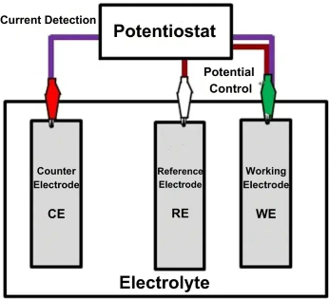
\includegraphics[width=0.6\linewidth]{figures/electrode.png}
    \caption{The three-electrode electrochemical cell configuration (working, reference and counter electrodes).}
    \label{fig:three_electrode}
\end{figure}

\mysubsection{Voltammetry as a family of techniques}{Voltammetry as a Family of Techniques (CV, LSV, SWV, DPV, Stripping Voltammetry)}
\label{sec:voltammetry_family}

In any voltammetric measurement, applying a voltage to an electrode generates two types of current:

\begin{itemize}
    \item \textbf{Faradaic current:} The actual current generated by the transfer of electrons during the oxidation or reduction of the target analyte \cite{alyamni2024}. This is the desired signal.
    \item \textbf{Charging (capacitive) current:} The background current generated simply by charging the electrical double-layer at the electrode surface, which acts like a capacitor caused by the Helmholtz plane \cite{alyamni2024}. This causes background noise.
\end{itemize}

The same three-electrode setup handles each of the following techniques in a different way:

\begin{itemize}
    \item \textbf{Linear Sweep (\ac{LSV}) and Cyclic Voltammetry (\ac{CV}):} The potentiostat applies a continuous, linear voltage ramp (or a triangular sweep for CV). The counter electrode continuously sinks or sources the resulting faradaic current.
    \item \textbf{Differential Pulse (\ac{DPV}) and Square Wave Voltammetry (\ac{SWV}):} Instead of a continuous ramp, the potentiostat applies a series of discrete voltage pulses or steps. By measuring the current at specific times during the pulse, the system can mathematically subtract the background capacitive (charging) current. This dramatically increases sensitivity, making DPV and SWV the preferred techniques for trace-level detection in biosensing applications.
    \item \textbf{Stripping voltammetry:} This is a two-step process that still relies on the exact same electrodes. First, the potentiostat holds a constant potential to electroplate (pre-concentrate) the analyte onto the working electrode. It then applies a sweep or pulse waveform (often an LSV, DPV, or SWV waveform) to ``strip'' the analyte back into the solution, yielding a large current spike.
\end{itemize}

\mysubsection{Differential pulse voltammetry theory}{Differential Pulse Voltammetry Theory}
\label{sec:dpv_theory}

\ac{DPV} superimposes small pulses of potential onto a linear potential ramp or staircase. The current difference is measured before and near the end of each pulse to reduce background charging current and achieve high sensitivity \cite{pineresearch_dpv}, although this comes at the cost of time resolution \cite{sciencedirect1993dpv}. DPV builds on the foundations of linear sweep methods; however, it uses a more complex, discontinuous voltage waveform.

\mysubsection{Waveform description}{Waveform Description (Pulse Height, Pulse Width, Step Potential, Current Sampling Windows)}
\label{sec:dpv_waveform}

In \ac{DPV}, the excitation waveform consists of a foundational staircase ramp with a discrete voltage pulse superimposed onto each step, as shown in Figure~\ref{fig:dpv_waveform}. The geometry of this waveform is defined by the pulse amplitude, which dictates the voltage magnitude of the superimposed pulse, and the pulse width, which specifies how long this elevated potential is held before the system returns to the baseline step potential.

Crucially, a potentiostat executing a DPV sweep does not measure current continuously. Instead, the analog front-end executes two precise, discrete current samples per cycle. The first sample ($I_{\text{before}}$) is recorded immediately before the pulse is applied, and the second sample ($I_{\text{end}}$) is captured at the end of the pulse duration. The final analytical output for that specific voltage step is derived by subtracting the baseline sample from the pulse sample, yielding a differential current
\begin{equation}
    \Delta I = I_{\text{end}} - I_{\text{before}}.
    \label{eq:dpv_diff}
\end{equation}
This differential data point is what is ultimately plotted against the applied step potential to form the voltammogram.

\begin{figure}[H]
    \centering
    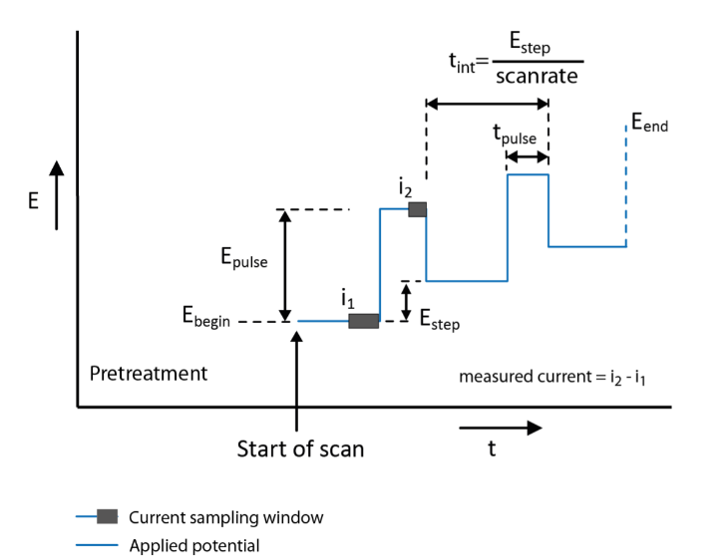
\includegraphics[width=0.7\linewidth]{figures/pulse.png}
    \caption{The \ac{DPV} excitation waveform, showing the staircase ramp, superimposed pulses, and the two current-sampling instants ($I_{\text{before}}$ and $I_{\text{end}}$) per step. }
    \label{fig:dpv_waveform}
\end{figure}

\mysubsection{Why DPV improves sensitivity}{Why DPV Improves Sensitivity / Reduces Background (Capacitive) Current Compared to LSV/CV}
\label{sec:dpv_sensitivity}

When a changing voltage occurs ($dV/dt$) over a brief period, a large spike in capacitive charging current occurs at the electrode-electrolyte interface. In continuous voltage sweeps such as CV or LSV, this capacitive noise is always present. The capacitive charging current decays exponentially as $e^{-t/RC}$, whereas the faradaic current decays much more slowly and is governed by the Cottrell equation, $1/\sqrt{t}$. To combat this, the second current measurement is taken at the end of the pulse width; this allows the double-layer capacitor time to fully charge so that the capacitive noise has died out, leaving only the faradaic signal. The resulting measurement has a much higher \ac{SNR}, allowing for the detection of much lower analyte concentrations. Analytes of interest span a large range of applications.

\mysubsection{Typical analytical applications}{Typical Analytical Applications (Trace Metals, Pharmaceuticals, Biosensing)}
\label{sec:dpv_applications}

Because \ac{DPV} effectively filters out capacitive charging current, it achieves exceptional sensitivity and low limits of detection, making it a foundational technique across multiple analytical fields. In environmental monitoring, DPV is frequently used in tandem with anodic stripping methods to detect trace heavy metals, such as lead and arsenic, at parts-per-billion concentrations in water systems. Within the pharmaceutical industry, it is used to analyse the purity of drug formulations and to study the oxidation mechanisms of active pharmaceutical ingredients. Furthermore, DPV is increasingly critical in the development of modern electrochemical biosensors. The biological fluids analysed in these systems (e.g.\ food or interstitial fluid) are highly resistive and generate significant background noise; by mathematically rejecting this noise, DPV allows microfluidic lab-on-a-chip devices to isolate the minute faradaic currents produced by specific biomarkers, enabling rapid and highly sensitive point-of-care diagnostics. All of these applications are controlled by a potentiostat.

\mysection{Potentiostat fundamentals}{Potentiostat Fundamentals}
\label{sec:potentiostat_fundamentals}

This section explores the fundamentals of a potentiostat, namely its role, design, performance parameters, and implementation approaches.

\mysubsection{The role of a potentiostat}{The Role of a Potentiostat}
\label{sec:role_potentiostat}

The role of a potentiostat is to control the control amplifier and the current-to-voltage amplifier (\ac{TIA}), and to buffer the reference electrode. For reference electrode buffering, the electrode must remain perfectly stable at a known half-cell potential; to prevent the voltage from drifting, zero current is allowed to flow through the electrode. This is achieved using an electrometer, an operational amplifier with an extremely high input impedance.

The control amplifier drives the system by constantly comparing the desired input voltage, set by a \ac{DAC}, with the actual voltage measured at the reference electrode. The resulting error signal is minimised by forcing current through the counter electrode and into the solution, which actively compensates for any changes in the electrochemical cell's resistance. The current-to-voltage converter (TIA) holds the working electrode at a 0\,V reference (virtual ground) while catching every electron produced or consumed by the reaction. These electrons generate a small faradaic current that is converted into a potential, which can then be measured by an \ac{ADC} \cite{bard2001}. Each of the three amplifiers is connected to one of the three electrodes.

\mysubsection{The classic 3-op-amp potentiostat topology}{The Classic 3-Operational Amplifier Potentiostat Topology}
\label{sec:3opamp_topology}

This section translates the three roles above into a physical circuit architecture, shown in Figure~\ref{fig:3opamp}.

\begin{itemize}
    \item \textbf{The feedback loop:} The 3-op-amp topology forms a negative feedback loop. The electrochemical cell itself (between the \ac{CE} and \ac{RE}) is physically placed inside the feedback path of the control amplifier.
    \item \textbf{Op-amp A (the driver):} The control amplifier.
    \item \textbf{Op-amp B (the buffer):} The RE voltage follower.
    \item \textbf{Op-amp C (the sensor):} The TIA connected to the WE.
\end{itemize}

\begin{figure}[H]
    \centering
    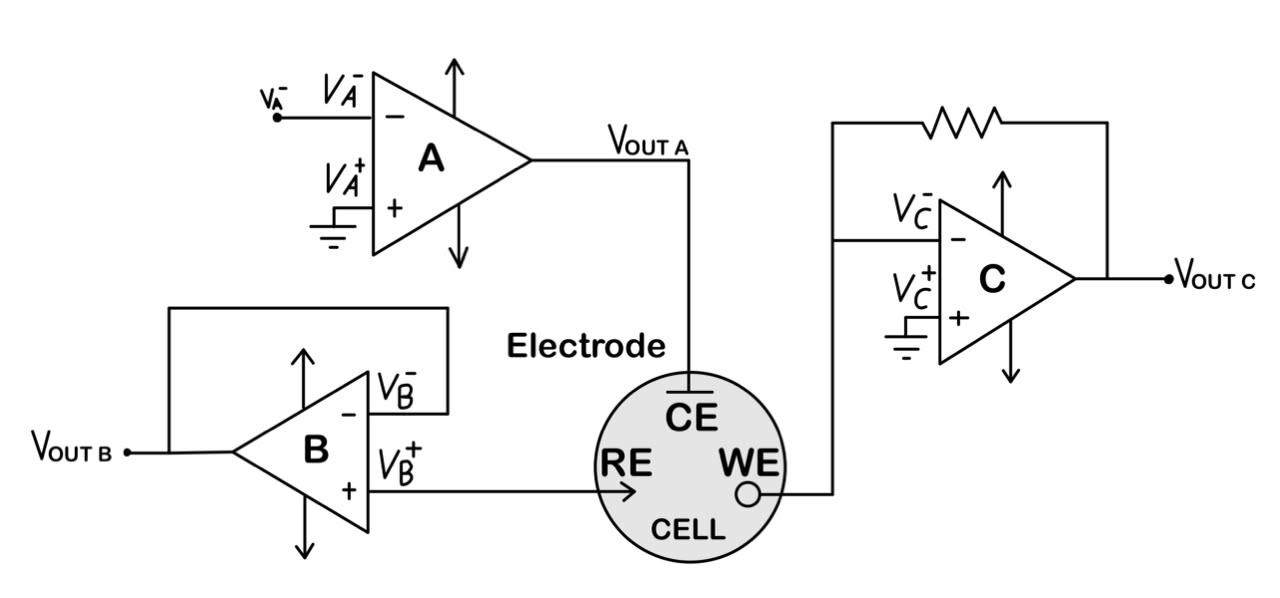
\includegraphics[width=0.7\linewidth]{figures/3opamp.jpeg}
    \caption{The classic 3-operational-amplifier potentiostat topology, showing the control amplifier, RE buffer, and TIA connected to the three electrodes.}
    \label{fig:3opamp}
\end{figure}

\mysubsection{Key performance parameters}{Key Performance Parameters}
\label{sec:key_performance_parameters}

This section establishes the criteria used to evaluate the effectiveness of the hardware, namely current measurement range and resolution, compliance voltage, noise floor, bandwidth, and technique support.

\begin{itemize}
    \item \textbf{Current measurement range and resolution:} In microfluidic biosensing, very small faradaic signals are generated. The potentiostat must be able to accurately measure down to the nanoampere (nA) or picoampere (pA) range without clipping or saturating the signal.

    \item \textbf{Compliance voltage:} This is the maximum voltage the control amplifier can physically output. Compliance voltage describes the ability of a power supply to push a much higher maximum voltage in order to keep a steady current flowing through a high-resistance load. If a fluid sample has high electrical resistance, the control amplifier needs a high compliance voltage to push the necessary current through the counter electrode.

    \item \textbf{Noise floor and \ac{LOD}:} The LOD of an electrochemical biosensor is fundamentally constrained by the inherent noise floor of the potentiostat's analog front end. In high-sensitivity applications, the TIA requires large feedback resistors to convert picoampere-level faradaic currents into measurable voltages. However, these resistive components inherently generate thermal (Johnson--Nyquist) noise, which scales with resistance and temperature. Therefore, a microfluidic diagnostic device targeting trace biomarkers (generating nanoampere or picoampere signals) requires a potentiostat topology with an exceptionally low electrical noise floor. If the peak-to-peak amplitude of the circuit's electronic noise exceeds the faradaic signal generated by the biomarker, reliable detection is physically impossible.

    \item \textbf{Bandwidth / scan rate limits:} This is the maximum speed at which the potentiostat can alter the applied potential. Fast techniques such as \ac{SWV} require high-bandwidth operational amplifiers to avoid signal distortion.

    \item \textbf{Technique support:} A system's ability to run CV, DPV, or \ac{EIS} depends on its \ac{DAC} resolution and internal waveform generators \cite{cruz2020}.
\end{itemize}

\mysubsection{Analog front-end approaches}{Analog Front-End Approaches}
\label{sec:afe_approaches}

Transitioning from the theoretical 3-op-amp topology to a physical implementation requires selecting an appropriate hardware architecture. While commercial benchtop potentiostats offer uncompromising analytical performance, their bulky form factors and high costs render them unsuitable for portable or point-of-care microfluidic diagnostics. Consequently, engineers developing custom electrochemical systems typically choose between two primary \ac{AFE} strategies: constructing a discrete circuit using individual operational amplifiers, or utilising a fully integrated \ac{SoC} AFE, such as the AD5941. Each approach presents distinct engineering trade-offs regarding power consumption, physical footprint, and architectural flexibility, which are summarised in Table~\ref{tab:afe_approaches}.

\begin{table}[H]
    \caption{Comparison of discrete op-amp and integrated AFE IC implementation approaches.}
    \footnotesize
    \centering
    \begin{tabular}{p{4cm}p{5cm}p{5cm}}
    \toprule
        \textbf{Implementation Approach} & \textbf{Advantages} & \textbf{Trade-offs} \\
    \midrule
        Discrete op-amp design &
        Unlimited architectural flexibility; capable of massive compliance voltages; component-level tuning for extreme precision &
        Large physical PCB footprint; high power consumption; complex board-level noise routing; higher cost of materials \\
        \addlinespace
        Integrated AFE ICs &
        Millimeter-scale physical footprint; ultra-low power consumption for \ac{IoT}; built-in hardware digital filtering; significantly lower per-unit cost &
        Hard-capped compliance voltage ($\leq 3$\,V); fixed internal current measurement ranges; black-box topology limits deep customisation; requires complex SPI/I2C firmware development \\
    \bottomrule
    \end{tabular}
    \label{tab:afe_approaches}
\end{table}

\mysection{Survey of existing potentiostat designs}{Survey of Existing Potentiostat Designs}
\label{sec:survey_designs}

The democratisation of electrochemical instrumentation has led to a rapid expansion of custom potentiostat designs. This section surveys the architectural evolution of these devices, establishing a performance baseline and identifying existing gaps in standalone usability and embedded intelligence.

\mysubsection{Commercial instruments}{Commercial Instruments}
\label{sec:commercial_instruments}

Commercial systems, such as the PalmSens EmStat or Metrohm Autolab, serve as the gold standard for electrochemical analysis. They offer uncompromising precision, massive dynamic ranges (pA to mA), rigorous factory calibration, and robust proprietary software suites. These instruments fall short in that they are cost-prohibitive (often exceeding thousands of dollars), physically bulky, and operate as closed-source devices, making them impossible to integrate deeply into custom, low-cost microfluidic or \ac{IoT} architectures. Nevertheless, they are exceedingly valuable in that they provide the foundational performance benchmarks against which all open-source and custom hardware must be validated \cite{palmsens2023}.

\mysubsection{Early open-source designs}{Early Open-Source Designs}
\label{sec:early_opensource}

The inception of open-source electrochemistry was marked by devices like the CheapStat \cite{rowe2011}. These devices proved that rudimentary analytical electrochemistry could be achieved with a \ac{BOM} under \$100, dramatically lowering the barrier to entry for educational and resource-limited settings. Since these first-generation potentiostats were built on early 8-bit microcontrollers, they suffered from poor \ac{ADC}/\ac{DAC} resolution, narrow voltage compliance windows, and a lack of wireless connectivity. CheapStat pioneered the open-hardware movement in electrochemistry, establishing the viability of DIY discrete op-amp topologies \cite{rowe2011}.

\mysubsection{General-purpose / high-performance open-source designs}{General-Purpose / High-Performance Open-Source Designs}
\label{sec:general_purpose_opensource}

To bridge the performance gap between early DIY builds and commercial units, high-performance open-source designs such as the DStat \cite{dryden2015} were developed. The DStat drastically improved noise performance, offered multi-technique support (CV, SWV, DPV, CA), and provided an excellent Python-based \ac{GUI}. Unfortunately, it remains tethered to a PC via USB for power and data processing; while highly accurate, this reliance on an external computer negates true field portability. This was the first time that custom discrete analog front-ends could achieve near-commercial sensitivity limits \cite{dryden2015}.

\mysubsection{Portable / wireless / smartphone-integrated designs}{Portable / Wireless / Smartphone-Integrated Designs}
\label{sec:portable_wireless}

The development of \ac{BLE} led to a generation of smartphone-integrated devices, such as the UWED and various ESP32-based We-VoltamoStat iterations \cite{ainla2018}. These devices achieved true field portability by offloading the processing and display requirements onto the user's smartphone, reducing the hardware footprint of the potentiostat itself. However, these designs are locked into their companion application: if the proprietary application is not maintained to support operating system updates, the hardware becomes obsolete \cite{ainla2018}. Furthermore, Bluetooth pairing can be unreliable in electrically noisy industrial environments \cite{automationworld_bluetooth}.

\mysubsection{EIS-capable / AFE-chip-based designs}{EIS-Capable / AFE-Chip-Based Designs}
\label{sec:eis_afe_designs}

The introduction of highly integrated, mixed-signal \acp{AFE} catalysed a shift away from bulky discrete op-amp circuits \cite{jenkins2019}. Systems like ABE-Stat, HunStat (2024), and HunStat2 (2025) characterise this generation. Utilising \acp{SoC} such as the AD5941 enables these devices to support complex, high-frequency techniques like \ac{EIS} while consuming fractions of a milliwatt; they boast exceptionally low electronic noise floors and millimeter-scale footprints \cite{hunstat2024,hunstat2_2025}. The development of ESP32 microcontrollers further aided performance as well as the appeal for DIY projects. However, the firmware required to configure the AFE registers is exceptionally complex, and devices such as HunStat are typically deployed as data-loggers; they lack built-in user interfaces and rely on raw serial data dumps for analysis. These two factors are an unfortunate downside of these systems \cite{hunstat2_2025}.

\mysubsection{Self-hosted web-interface / onboard-display designs}{Self-Hosted Web-Interface / Onboard-Display Designs}
\label{sec:selfhosted_webinterface}

To solve the challenge of being locked into a companion app, recent ESP32-based potentiostats have integrated embedded web servers. NanoStat \cite{lee2022} hosts an HTML5/JavaScript server, meaning any Wi-Fi-enabled device can control it via a standard browser. DM-Stat \cite{dmstat2024} and SaxStat \cite{saxstat2025} follow similar ``OpenEChem'' philosophies. A major benefit of this approach is ultimate cross-platform compatibility (Windows, macOS, iOS, Android) without requiring the user to install any software; however, hosting a web server consumes significant \ac{MCU} RAM and flash memory \cite{lee2022}.

There is a potential novelty gap in including a physical onboard display in such a system. A review of these systems reveals that they are almost exclusively headless. This highlights a distinct gap in the literature: a dual-interface approach would allow for rapid, standalone field testing without requiring the user to reach for a smartphone, while still preserving web-based data extraction capabilities.

\mysubsection{Machine-learning-assisted voltammetry}{Machine-Learning-Assisted Voltammetry}
\label{sec:ml_voltammetry}

The most recent paradigm shift involves embedding \ac{ML} algorithms directly onto the potentiostat's microcontroller. Examples include embedded multi-layer perceptrons for heavy-metal stripping voltammetry and models classifying \ac{DPV} responses for Dengue/Zika biomarkers on highly constrained hardware ($<$10\,kB RAM) \cite{mlheavymetal,mldengue}. Such models shift the system from mere data \textit{collection} to on-device data \textit{interpretation}, allowing the device to output actionable results (e.g.\ ``positive/negative'' or specific concentrations) rather than forcing a human expert to interpret a noisy voltammogram. These systems are less attractive in that they require extensive prior data collection to train the models, and inference algorithms consume heavy compute cycles on standard MCUs.

Table~\ref{tab:design_comparison} summarises the surveyed designs against the proposed architecture for this project.

\begin{table}[H]
    \caption{Comparison of surveyed potentiostat designs against the proposed architecture.}
    \tiny
    \centering
    \begin{tabular}{
        >{\raggedright\arraybackslash}p{2.3cm}
        >{\raggedright\arraybackslash}p{2.3cm}
        >{\raggedright\arraybackslash}p{2.6cm}
        >{\raggedright\arraybackslash}p{2.3cm}
        >{\raggedright\arraybackslash}p{1.5cm}
        >{\raggedright\arraybackslash}p{1.5cm}
        >{\raggedright\arraybackslash}p{2cm}
    }
    \toprule
        \textbf{Design / Platform} & \textbf{MCU / AFE Architecture} & \textbf{Primary Techniques Supported} & \textbf{Connectivity \& Interface} & \textbf{Onboard Display?} & \textbf{ML / Onboard Analysis?} & \textbf{Open-Source Completeness} \\
    \midrule
        Commercial (e.g.\ EmStat) & Proprietary & CV, DPV, SWV, EIS, CA & USB / Proprietary PC GUI & No & No (PC-based) & Closed source \\
        CheapStat (2011) & Atmel AVR / Discrete & CV, SWV, CA & None / Basic LCD output & Yes (Basic LCD) & No & Full (PCB/Firmware) \\
        DStat (2015) & Atmel XMEGA / Discrete & CV, DPV, SWV, CA & USB / Python PC GUI & No & No & Full (PCB/Firmware/GUI) \\
        Smartphone-Integrated (e.g.\ UWED) & BLE MCU / Discrete & CV, DPV, SWV & Bluetooth / Custom App & No & No & Partial (Hardware focus) \\
        HunStat2 (2025) & Mixed / AD5941 SoC & CV, DPV, SWV, EIS & USB / Serial Datalogging & No & No & Full (Hardware/Firmware) \\
        NanoStat (2022) & ESP32 / Discrete & CV, SWV, CA & Wi-Fi / Embedded Web GUI & No (Headless) & No & Full (Hardware/Web GUI) \\
        \textbf{Proposed ML Architecture} & ESP32 / AD5941 SoC & CV, DPV, SWV & Wi-Fi Web GUI + Standalone & Yes & Yes (Edge ML) & TBD \\
    \bottomrule
    \end{tabular}
    \label{tab:design_comparison}
\end{table}

%
\mychapter{System Modeling \& Theoretical Design}{System Modeling \& Theoretical Design}{}
\label{chap:Overall-System-Design-and-Modeling}

\section{System Architecture}
The proposed hardware architecture of the potentiostat is illustrated in Figure \ref{fig:system_architecture} is divided into high-level software logic and discrete hardware components. The architecture is designed to be modular, allowing for easy integration of various components. The analog front-end serves as the core of the system, providing the necessary tools for electrochemical measurements. The microcontroller manages data acquisition, processing, and communication. The physical user interface allows for local control and user input and control. The three-electrode setup ensures accurate electrochemical measurements, making the system suitable for detecting trace levels of antiretroviral medications in water samples.

The software architecture manages the analytical core and connectivity of the system. It is driven by real-time operating system and features an embedded web server and Wi-Fi capabilities for data extraction and review alongside data storage. The analytical core manages the DPV waveform generation and differential current calculations, while a local GUI and display driver ensure the physical interface is operational without the need for an external smart device.

\begin{figure}[H]
    \centering
    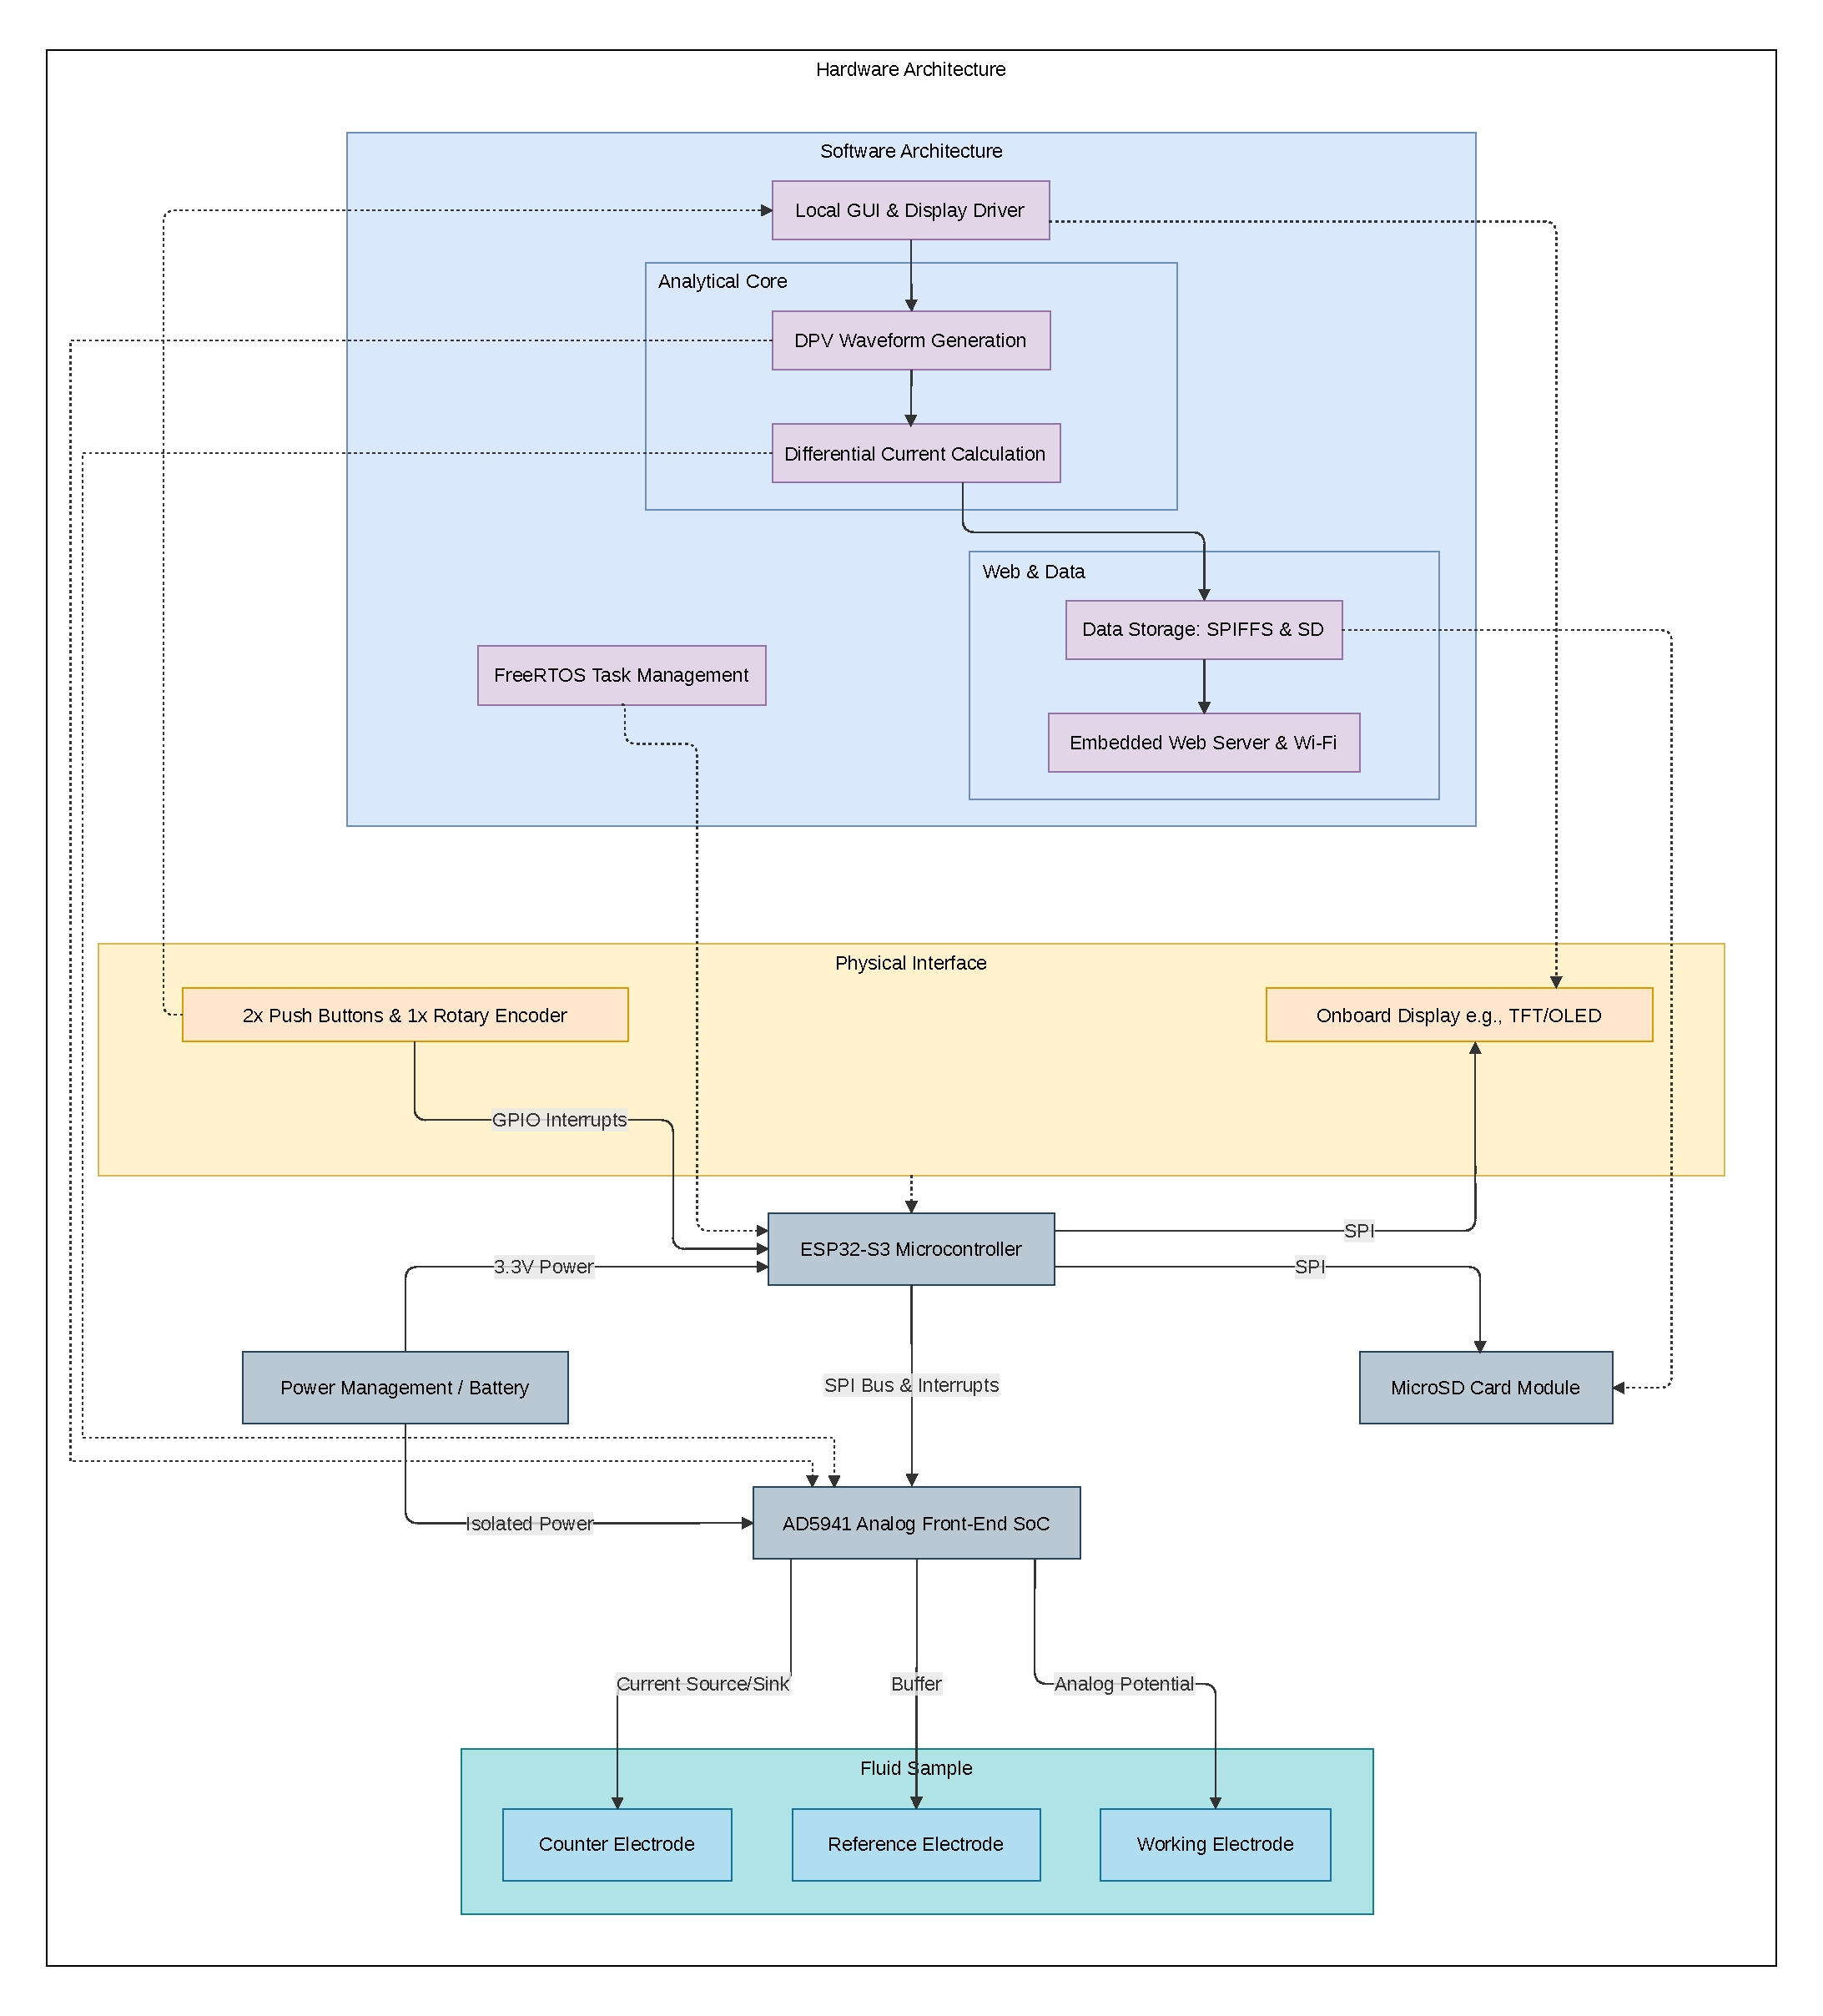
\includegraphics[width=0.9\textwidth]{figures/SystemArchitecture.pdf}
    \caption{System Architecture Diagram}
    \label{fig:system_architecture}
\end{figure}


\section{Electrochemical Cell \& Equivalent Circuit Modeling}
% Focus: Transforming electrochemistry into an electrical model.

% TODO: Model the three-electrode cell using a Randles Equivalent Circuit.
% Discuss solution resistance (R_s), double-layer capacitance (C_{dl}), and charge-transfer resistance (R_{ct}).

It is possible to model the electrochemical cell as a Randle's equivalent circuit, as seen in Figure \ref{fig:randles_circuit}. After defining the system architecture required to interface with the electrochemical cell, it is required to mathematically model what the cell presents to the system. The Randle equivalent circuit is a complex non-ideal impedance model that changes depending on frequency, applied potential and the electrochemical reaction occurring at the working electrode. To design a control loop capable of driving this load reliably, the cell must first be reduced to an equivalent electrical model. A widely used representation of the cell is the Randles equivalent circuit \cite{Laschuk2021}. This equivalent circuit models the electrode and electrolyte interface as a series solution resistance ($R_s$) in series with a parallel combination of the double-layer capacitance ($C_{dl}$) and the charge-transfer resistance ($R_{ct}$). The Warburg impedance ($Z_W$) is included to account for diffusion effects at low frequencies. This model allows for the analysis of the electrochemical cell's behavior under different conditions and is essential for designing the potentiostat's control loop \cite{sannino2025potentiostat}.


% Mathematically derive why pulse voltammetry (like DPV) isolates faradaic analytical current from capacitive charging current based on their exponential decay time constants.

\begin{figure}[H]
    \centering
    \begin{circuitikz}[american, thick]
        % Input from Working Electrode (WE)
        \draw (0,0) node[anchor=east] {WE} to[short, o-] (0.5,0)
        % Solution Resistance (Rs)
        to[R, l=$R_s$] (2.5,0);
        
        % Split into parallel branches
        % Top branch: Double Layer Capacitance (Cdl)
        \draw (2.5,0) -- (2.5,1.5) 
        to[C, l=$C_{dl}$] (6.5,1.5) -- (6.5,0);
        
        % Bottom branch: Charge Transfer Resistance (Rct) and Warburg (Zw)
        \draw (2.5,0) -- (2.5,-1.5) 
        to[R, l=$R_{ct}$] (4.5,-1.5)
        to[generic, l=$Z_W$] (6.5,-1.5) -- (6.5,0);
        
        % Output to Counter/Reference Electrode (CE/RE)
        \draw (6.5,0) to[short, -o] (7,0) node[anchor=west] {CE/RE};
    \end{circuitikz}
    \caption{Randles equivalent circuit modeling the electrochemical cell interface.}
    \label{fig:randles_circuit}
\end{figure}

The link between DPV waveforms and the Randles equivalent circuit is found through identifying the electrical demand it places on the potentiostat. The combination of the $R_s$ and $R_{ct}$ resistors is the total resistive load that must be driven by the control amplifier to sustain the target faradaic current. This resistive load dictates the compliance voltage that the system requires \cite{pineresearch_compliance}. The combination of $R_s$ and $C_{dl}$ form a RC time constant which dictates how quickly the double layer capacitance charges after each step in potential. This time constant governs how long a DPV pulse should be held to ensure that the background current has sufficiently decayed relative to the faradaic current \cite{bard2001}. Rather than being arbitrary selections, parameters such as pulse width, TIA gain, and control-amplifier bandwidth are strictly dictated by the expected $R_s$, $C_{dl}$, and $R_{ct}$ values of the target analyte-electrode interface. If the sampling scheme or amplifier bandwidth fails to match this characteristic RC time constant, the system cannot effectively filter out the unwanted capacitive component of the measured current\cite{sannino2025potentiostat}.

\subsection{Proving Capacitive Current Rejection in DPV}

DPV's effectiveness relies on the different decay rates of the two current components generated at an electrode following a potential step.

\subsubsection{Total Current at the Electrode}

When a potential step is applied, the total measured current is the sum of the faradaic and capacitive components:

\begin{equation}
I_{total}(t) = I_f(t) + I_c(t)
\end{equation}

\begin{table}[htbp]
\centering
\begin{tabular}{l l l l}
\toprule
\textbf{Current Type} & \textbf{Source} & \textbf{Decay Function} & \textbf{Decay Rate} \\
\midrule
Capacitive ($I_c$) & \makecell[l]{Charging the electrical \\ double layer} & $e^{-t/RC}$ & \makecell[l]{Very fast \\ (exponential)} \\
\addlinespace
Faradaic ($I_f$) & \makecell[l]{Electron transfer} & $1/\sqrt{t}$ & \makecell[l]{Slower \\ (inverse square root)} \\
\bottomrule
\end{tabular}
\caption{Comparison of Capacitive and Faradaic Currents}
\label{tab:current_types}
\end{table}

The capacitive current models the electrode-solution interface as an $RC$ circuit, decaying exponentially \cite{palmsens_capacitive_current}:

\begin{equation}
I_c(t) = \frac{\Delta E}{R_s} \, e^{-t/R_sC_{dl}}
\end{equation}

Where: 
\begin{itemize}

\item $R_s$ is the solution resistance.
\item $C_{dl}$ is the double-layer capacitance.
\item $\Delta E$ is the applied potential step.

\end{itemize}

The faradaic current is governed by the Cottrell equation for planar diffusion, decaying with the inverse square root of time \cite{bard2001}:

\begin{equation}
I_f(t) = \frac{nFA\sqrt{D}\,C^*}{\sqrt{\pi t}}
\end{equation}

Where: 

\begin{itemize}
    \item $n$ is the number of electrons transferred.
    \item $F$ is Faraday's constant.
    \item $A$ is the electrode area.
    \item $D$ is the diffusion coefficient.
    \item $C^*$ is the bulk analyte concentration.
\end{itemize}

Because an exponential function ($e^{-t/RC}$) tends toward zero faster than an inverse square root function ($1/\sqrt{t}$), by waiting for a sufficient amount of time after applying the pulse ensures the capacitive current disappeared while the faradaic current remains. 
\subsubsection{The Pulse-Sampling Scheme}

To utilise the property difference between the two current types, DPV applies a series of short voltage pulses superimposed on a linear staircase ramp. To isolate the faradaic current, the potentiostat samples the current twice per pulse cycle:

\begin{enumerate}
    \item $I_{before}$: sampled just before the pulse is applied.
    \item $I_{end}$: sampled at the very end of the pulse duration ($t = \tau_{pulse}$).
\end{enumerate}

\subsubsection{The Differential Proof}

The final output plotted in a DPV voltammogram is the difference between these two samples:

\begin{equation}
\Delta I = I_{end} - I_{before}
\end{equation}

Expanding using the component currents:

\begin{equation}
\Delta I = \left(I_{f,end} + I_{c,end}\right) - \left(I_{f,before} + I_{c,before}\right)
\end{equation}

Finding a solution to the decay mathematics to solve the problem:

\begin{itemize}
    \item Since $I_{before}$ is sampled just before the pulse, the system has been at a baseline potential for a sufficient amount of time so that any previous capacitive transient current has decayed completely. Thus, $I_{c,before} \approx 0$.
    \item Since $I_{end}$ is sampled at the very end of the pulse duration, the new capacitive transient caused by the pulse has also decayed to near zero. Thus, $I_{c,end} \approx 0$.

\end{itemize}

Therefore, the differential in Equation 3.5 simplifies to:

\begin{equation}
\Delta I \approx I_{f,end} - I_{f,before}
\end{equation}

By subtracting $I_{before}$ from $I_{end}$, DPV mathematically rejects the background charging current, leaving only the faradaic signal of interest.

\subsubsection{Why the Output Forms a Peak}

Because $\Delta I$ represents the change in faradaic current for a small, discrete step in potential ($\Delta E$), the resulting plot of $\Delta I$ versus $E$ is effectively an approximation of the derivative of a standard current-potential curve:

\begin{equation}
\Delta I \approx \frac{dI_f}{dE} \cdot \Delta E
\end{equation}

For a reversible system (electron transfer is so fast the system is always in thermodynamic equilibrium) governed by the Nernst equation, taking the derivative of the standard sigmoidal voltammogram produces a Gaussian-like peak. This peak reaches its maximum amplitude exactly at the half-wave potential ($E_{1/2}$), providing an incredibly sensitive and easily quantifiable signal \cite{Laborda2014}.


\section{Analog Front-End Stability \& Control Loop Modeling}
% Focus: Ensuring the potentiostat feedback loop is stable and noise-free.

% TODO: Detail how the double-layer capacitance (C_{dl}) adds a pole to the feedback path, threatening loop stability. 
% Derive the transfer function of the transimpedance amplifier (TIA).

The generalized transfer function for the transimpedance amplifier is defined as:
\begin{equation}
    H(s) = \frac{V_{\text{out}}(s)}{I_{\text{in}}(s)} = - \frac{R_f}{1 + s R_f C_f}
    \label{eq:tia_transfer}
\end{equation}

\subsection{Impact of C\textsubscript{dl} on TIA Loop Stability}

The working electrode connects directly to the summing junction (virtual ground) of the transimpedance amplifier (TIA). Because the double-layer capacitance, $C_{dl}$, physically exists between the working electrode and the bulk solution, it appears electrically as a shunt capacitance from the TIA's inverting input node to ground -- functionally identical to the junction capacitance of a photodiode in a conventional TIA design \cite{graeme1996}. This section derives the TIA transfer function to show how $C_{dl}$ introduces an additional pole into the feedback loop, degrading phase margin and threatening stability.

\subsubsection{Circuit Model and Node Equation}

Let $R_f$ be the TIA feedback resistor, $C_{dl}$ the shunt capacitance at the inverting node, and $A(s)$ the open-loop gain of the operational amplifier. Let $V_n$ be the voltage at the inverting node and $I_{in}$ the faradaic current sourced by the electrochemical reaction. Applying KCL at the summing node:

\begin{equation}
I_{in} = V_n \, sC_{dl} + \frac{V_n - V_{out}}{R_f}
\label{eq:kcl}
\end{equation}

Since the op-amp enforces $V_{out} = -A(s)V_n$ (with the non-inverting input grounded), we have:

\begin{equation}
V_n = -\frac{V_{out}}{A(s)}
\label{eq:vn}
\end{equation}

Substituting Equation~\eqref{eq:vn} into Equation~\eqref{eq:kcl} and solving for $V_{out}/I_{in}$ gives the closed-loop transimpedance:

\begin{equation}
Z_T(s) \equiv \frac{V_{out}}{I_{in}} = \frac{-R_f}{1 + \dfrac{1 + sR_fC_{dl}}{A(s)}}
\label{eq:ZT}
\end{equation}

\subsubsection{Noise Gain and the Loop Gain Pole}

Define the \emph{noise gain} of the feedback network as:

\begin{equation}
NG(s) = 1 + sR_fC_{dl}
\label{eq:NG}
\end{equation}

Equation~\eqref{eq:NG} shows that $C_{dl}$ introduces a \emph{zero} into the noise gain at:

\begin{equation}
f_z = \frac{1}{2\pi R_f C_{dl}}
\label{eq:fz}
\end{equation}

Above $f_z$, the noise gain rises at $+20\,\mathrm{dB/decade}$. The op-amp itself is modelled as a single-dominant-pole system, $A(s) = \omega_t/s$ near the crossover region, where $\omega_t = 2\pi \, \text{GBW}$ is the unity-gain angular frequency. The loop gain is therefore:

\begin{equation}
T(s) = \frac{A(s)}{NG(s)} = \frac{\omega_t}{s(1+sR_fC_{dl})}
\label{eq:loopgain}
\end{equation}

Equation~\eqref{eq:loopgain} reveals the core stability problem: the zero that $C_{dl}$ introduced into the noise gain (Eq.~\eqref{eq:NG}) becomes an additional \emph{pole} in the loop gain, located at:

\begin{equation}
\omega_{p2} = \frac{1}{R_f C_{dl}}
\end{equation}

Combined with the op-amp's intrinsic pole at the origin (from the integrator-like $\omega_t/s$ term), the loop gain $T(s)$ now contains \emph{two} poles below the crossover frequency.

\subsubsection{Phase Margin Degradation}

The closed-loop crossover frequency $\omega_{cl}$, where $|T(j\omega_{cl})| = 1$, is found by setting the magnitude of Equation~\eqref{eq:loopgain} to unity. For $\omega_{cl} \gg 1/(R_fC_{dl})$ (the typical high-bandwidth case):

\begin{equation}
|T(j\omega)| \approx \frac{\omega_t}{\omega^2 R_f C_{dl}} = 1
\quad \Longrightarrow \quad
\omega_{cl} = \sqrt{\frac{\omega_t}{R_f C_{dl}}}
\label{eq:wcl}
\end{equation}

At this crossover frequency, each of the two poles in $T(s)$ contributes close to $-90^\circ$ of phase shift, for a combined phase approaching $-180^\circ$. Since a negative feedback loop becomes unstable once the total loop phase reaches $-180^\circ$ at the frequency where $|T(j\omega)|=1$, the phase margin,

\begin{equation}
\phi_{PM} = 180^\circ - \left|\angle T(j\omega_{cl})\right|,
\end{equation}

collapses toward $0^\circ$. In practice this manifests as pronounced ringing, overshoot, or sustained oscillation in the measured current whenever the electrode's $C_{dl}$ is large relative to $1/(\omega_t R_f)$ -- precisely the condition encountered with high-sensitivity potentiostat designs, where $R_f$ must be large (to resolve nA--pA faradaic currents) and $C_{dl}$ can range from nanofarads to microfarads depending on electrode area and surface roughness \cite{ying2021}.

\subsubsection{Compensation}

Stability is restored by adding a small feedback capacitor $C_f$ in parallel with $R_f$, introducing a compensating pole into the noise gain \emph{before} the $C_{dl}$-induced zero dominates. Choosing $C_f$ such that the noise gain pole occurs at the geometric mean of $f_z$ and the amplifier's gain-bandwidth product restores a single-pole roll-off at crossover, yielding a phase margin close to $45^\circ$--$65^\circ$ \cite{graeme1996}:

\begin{equation}
C_f = \sqrt{\frac{C_{dl}}{2\pi R_f \, \text{GBW}}}
\label{eq:Cf}
\end{equation}

Equation~\eqref{eq:Cf} demonstrates that the compensation capacitor required for stable operation is a direct function of the electrode's double-layer capacitance, reinforcing that the electrochemical cell -- modelled via the Randles equivalent circuit -- is not merely a passive measurement target but an active determinant of the analog front-end's stability margin.

% TODO: Demonstrate how selecting the correct feedback resistor (R_f) and filtering capacitor (C_f) optimizes noise performance and phase margin.

\section{Voltammetric Digital Signal Processing \& Peak Extraction}
% Focus: The direct, deterministic replacement for the Machine Learning section.

% TODO: Map out the classical DSP pipeline. Define the mathematical subtraction formula for DPV.
The differential current is calculated as:
\begin{equation}
    \Delta I = I_{\text{end}} - I_{\text{before}}
    \label{eq:dpv_subtraction}
\end{equation}

% TODO: Detail the digital smoothing model (e.g., a Moving Average or Savitzky-Golay filter). 
% Formulate a derivative-based peak-finding algorithm combined with baseline linear interpolation.

The exact peak potential is automatically isolated by solving for the root of the derivative:
\begin{equation}
    \frac{d(\Delta I)}{dE} = 0
    \label{eq:peak_finding}
\end{equation}

\section{Embedded Communication Protocol \& GUI State Machine}
% Focus: Modeling the software interaction and state-tracking.

% TODO: Define the packet-level SPI communication protocol between the ESP32-S3 and the AD5941 registers.
% Present a formal finite state machine (FSM) or state transition model showing how the system handles asynchronous tasks (managing active scans, physical display refresh, WebSocket streaming) without disrupting ADC timing.

\begin{figure}[H]
    \centering
    % \includegraphics[width=0.8\textwidth]{figures/state_machine.png}
    \caption{Finite state machine diagram for managing asynchronous tasks and WebSocket communication.}
    \label{fig:gui_fsm}
\end{figure}
\providecommand{\swtodo}[1]{\textbf{[TODO: #1]}}

\usetikzlibrary{arrows.meta, positioning, calc, shapes.geometric, fit, patterns}

\tikzset{
  swbase/.style={draw, align=center, font=\footnotesize, inner sep=3pt,
                 line width=0.5pt,
                 execute at begin node={\hyphenpenalty=10000\relax\exhyphenpenalty=10000\relax}},
  swproc/.style={swbase, rectangle, minimum height=7mm, text width=#1},
  swproc/.default=34mm,
  swterm/.style={swbase, rectangle, rounded corners=3.4mm,
                 minimum height=7mm, text width=#1},
  swterm/.default=30mm,
  swdec/.style={swbase, diamond, aspect=2.4, inner sep=0.5pt, text width=#1},
  swdec/.default=24mm,
  % predefined process (detailed in another figure): box with side bars
  swsub/.style={swproc=#1, inner xsep=4.5mm,
    path picture={
      \draw[line width=0.5pt]
        ([xshift=1.6mm]path picture bounding box.north west) --
        ([xshift=1.6mm]path picture bounding box.south west)
        ([xshift=-1.6mm]path picture bounding box.north east) --
        ([xshift=-1.6mm]path picture bounding box.south east);}},
  swsub/.default=30mm,
  swarr/.style={-{Latex[length=2mm]}, line width=0.5pt},
  swdbl/.style={{Latex[length=2mm]}-{Latex[length=2mm]}, line width=0.5pt},
  swlbl/.style={font=\scriptsize, inner sep=1.5pt},
  swhw/.style={swbase, rectangle, minimum height=8mm, text width=#1,
               fill=black!10},
  swhw/.default=26mm,
}


% =====================================================================
%  Chapter 3 -- System Modeling & Theoretical Design
%
%  The Randles model and the capacitive current rejection derivation
%  now live in Chapter 2 (sec:cell_model and sec:dpv_theory).
%  The label sec:dpv_rejection was moved with them, so references to it
%  in Chapters 5 and 6 now point to the DPV subsection in Chapter 2.
% =====================================================================

\chapter{System Modeling \& Theoretical Design}
\label{chap:modeling}

This chapter presents the potentiostat designed for this project, referred to as the OpenStat. The OpenStat combines an integrated analog front-end, a browser interface and a standalone onboard display in a single handheld instrument. Section~\ref{sec:architecture} describes its architecture and the role of each part. Section~\ref{sec:afe_stability} then analyses the stability of the two amplifier loops that drive and measure the cell, which sets the requirements for the hardware in Chapter~\ref{chap:hardware_design} and the firmware in Chapter~\ref{chap:software_design}.

%------------------------------------------------------------------
\section{System Architecture}
\label{sec:architecture}

The OpenStat is built around two key elements. An AD5941 analog front-end applies the potential to the three-electrode cell and measures the resulting current. An ESP32-S3 controls the AD5941 over SPI, times the DPV waveform, computes the differential current and stores the results. The AD5941 was selected over a discrete design because it integrates the control amplifier, RE buffer and TIA of Section~\ref{sec:3opamp_topology} on a single chip, together with a 12-bit DAC, a 16-bit ADC and eight programmable gain ranges, at sub-milliwatt power in a millimetre-scale package. Its main limitation, the capped compliance voltage, does not restrict this application. In addition to these key elements are the interfaces that make the instrument standalone, namely a TFT display and SD card, the user interface, and a web server that serves results over Wi-Fi. Figure~\ref{fig:architecture} shows how the firmware connects these parts, with a single main loop servicing the measurement, display and web server in turn.

\begin{figure}[H]
  \centering
  \caption{Software architecture.
    Arrows show the direction of calls or data.}
  \label{fig:architecture}
  \begin{tikzpicture}[x=1cm, y=1cm]
    % --- external, top
    \node[swhw=30mm] (browser) at (7.6, 6.9) {Browser dashboard};
    \node[swhw=26mm] (pc)      at (12.8, 6.9) {Serial terminal};
    % --- row A
    \node[swproc=36mm] (screens) at (2.3, 5.0) {Screens and screen\\state machine};
    \node[swproc=34mm] (web)     at (7.6, 5.0) {Web server\\(HTTP, WebSocket)};
    \node[swproc=26mm] (serial)  at (12.8, 5.0) {Serial bench\\commands};
    % --- row B
    \node[swproc=16mm] (input)  at (0.5, 3.0) {Input\\manager};
    \node[swproc=46mm, minimum height=10mm] (engine) at (7.6, 3.0)
      {\textbf{Sweep engine}\\result buffer and storage};
    \node[swproc=26mm] (params) at (12.8, 3.0) {Scan parameters\\(saved in NVS)};
    % --- row C
    \node[swproc=22mm] (render) at (3.1, 1.0) {Renderer};
    \node[swproc=26mm] (driver) at (12.0, 1.0) {AD5941 driver};
    % --- firmware boundary
    \node[draw, dashed, line width=0.5pt, inner sep=3mm,
          fit=(screens)(serial)(input)(render)(driver)(params)] (fw) {};
    \node[swlbl, anchor=south west, font=\footnotesize\itshape]
      at ([yshift=0.3mm]fw.north west) {ESP32-S3 firmware};
    % --- hardware, bottom
    \node[swhw=16mm] (enc)  at (0.5, -1.1) {Encoder,\\buttons};
    \node[swhw=22mm] (tft)  at (3.1, -1.1) {TFT display};
    \node[swhw=24mm] (sd)   at (7.6, -1.1) {microSD card};
    \node[swhw=26mm] (afe)  at (12.0, -1.1) {AD5941 AFE};
    % --- connections
    \draw[swdbl] (browser) -- node[swlbl, right] {Wi-Fi} (web);
    \draw[swdbl] (pc) -- node[swlbl, right] {USB} (serial);
    \draw[swarr] (enc) -- node[swlbl, right, align=left, pos=0.12] {GPIO,\\interrupts} (input);
    \draw[swarr] (input.north) -- node[swlbl, left] {events}
      (input.north |- screens.south);
    \draw[swarr] ([xshift=-4mm]render.north |- screens.south) --
      node[swlbl, left, pos=0.3] {draw} ([xshift=-4mm]render.north);
    \draw[swdbl] ([xshift=16mm]screens.south) |-
      node[swlbl, right, pos=0.22] {callbacks} (engine.west);
    \draw[swarr] ([xshift=-17mm]engine.south) |-
      node[swlbl, above, pos=0.75] {live trace} (render.east);
    \draw[swdbl] (web) -- node[swlbl, left] {commands, points} (engine);
    \draw[swarr] (serial.south) -- ++(0,-0.5) -| ([xshift=17mm]engine.north);
    \draw[swdbl] (params) -- (engine);
    \draw[swarr] ([xshift=17mm]engine.south) |- (driver.west);
    \draw[swarr] (render) -- node[swlbl, right, pos=0.72] {SPI (HSPI)} (tft);
    \draw[swdbl] (engine) -- node[swlbl, right, pos=0.86] {SPI (HSPI)} (sd);
    \draw[swdbl] (driver) --
      node[swlbl, right, align=left, pos=0.72] {SPI (FSPI),\\\SI{4}{\mega\hertz}} (afe);
  \end{tikzpicture}
\end{figure}

The hardware that implements this architecture is described in Chapter~\ref{chap:hardware_design} and the firmware in Chapter~\ref{chap:software_design}. The rest of this chapter considers whether the analog front-end remains stable when the electrochemical cell is connected to it.

% ---------------------------------------------------------------------
\section{Analog Front-End Stability}
\label{sec:afe_stability}

The AD5941 implements the three-amplifier topology of Section~\ref{sec:3opamp_topology}. Its potentiostat amplifier acts as the control amplifier driving the CE, the RE is sensed through a high-impedance unity-gain stage, and the high-speed TIA holds the WE at virtual ground and converts the cell current to a voltage. The Randles model of Section~\ref{sec:cell_model} places specific demands on these amplifiers. The total resistance $R_s + R_{ct}$ sets the compliance voltage that the control amplifier must provide \cite{pineresearch_compliance}, and the time constant $R_sC_{dl}$ sets how long a DPV pulse must be held before the capacitive current has decayed \cite{bard2001}. The cell also lies inside the feedback loops of both the control amplifier and the TIA, so $C_{dl}$ affects the stability of each.

Each loop is assessed with the phase-margin criterion. The loop gain
$L(s) = A(s)\beta(s)$ is evaluated at the crossover frequency $\omega_c$,
where $|L(j\omega_c)| = 1$, and the phase margin
$\phi_\text{PM} = \SI{180}{\degree} + \angle L(j\omega_c)$ must be positive
for the loop to be stable, with \SIrange{45}{65}{\degree} giving a
well-damped response \cite{c2}. Both amplifiers are modeled with a single
dominant pole, $A(s) = \omega_t/s$ with $\omega_t = 2\pi \cdot
\text{GBW}$ \cite{bard2001}. The underlying feedback theory and the
derivations of the results below are given in Appendix~\ref{app:feedback}.

\subsection{Control Loop}
\label{sec:control_loop}

Only the high-frequency behaviour of the cell matters for stability. $R_{ct}$
and $Z_W$ in Figure~\ref{fig:randles_circuit} govern the slow Faradaic
response and are omitted, which reduces the cell to $C_{dl}$ in series with
the uncompensated resistance $R_u$, the part of $R_s$ between the RE and the
WE \cite{bard2001, c7, c8}. This reduced cell is shown in
Figure~\ref{fig:cell_buffer}.

\begin{figure}[H]
    \centering
    \caption{Electrochemical cell equivalent circuit interfaced with the reference electrode buffer.}
    \label{fig:cell_buffer}
    \begin{circuitikz}[american, thick]
        
        % Block style for the RE buffer
        \tikzset{
            re_block/.style={
                rectangle,
                draw=teal!50!black,
                fill=teal!80!black,
                text=white,
                rounded corners=3pt,
                minimum width=3.8cm,
                minimum height=1.2cm,
                align=center
            }
        }

        % 1. Left wire and CE node (Shifted left for clearance)
        \draw (2,0) -- (0.5,0);
        \fill (0.5,0) circle (2.5pt);
        \node[above=0.15cm] at (0.5,0) {\textbf{CE}};
        \node[below=0.15cm] at (-0.2,0) {\textsf{$e_o(s)$, Op-Amp A}};
        
        % Wire entering the dashed box
        \draw (0.5,0) -- (2.0,0);
        
        % 2. Resistor Ru
        \draw (2.0,0) to[R, l=$R_u$] (4.5,0);
        
        % 3. Center Tap (to RE buffer)
        \fill (4.5,0) circle (2.5pt);
        
        % 4. Capacitor Cdl
        \draw (4.5,0) to[C, l=$C_{dl}$] (7.0,0);
        
        % 5. Right wire, WE node, and Ground
        \draw (7.0,0) -- (8.5,0);
        \fill (8.5,0) circle (2.5pt);
        \draw (8.5,0) node[ground]{}; 
        
        % Adjusted WE label position to not clash with ground symbol
        \node[below=0.85cm, align=center] at (8.5,0) {\textbf{WE}\\ \textsf{Virtual ground (Op-Amp C, TIA)}};
        
        % 6. Dashed Box for Electrochemical Cell
        % Adjusted dimensions to encompass R and C properly and leave room for text
        \draw[dashed, draw=gray!80, thick] (1.6, -1.3) rectangle (7.4, 1.6);
        
        % Text shifted slightly inside the box so it doesn't overlap the border
        \node[anchor=north west, text=gray!90] at (1.7, -0.5) {\textsf{Electrochemical cell ($R_u$, $C_{dl}$)}};
        
        % 7. RE Buffer Block
        \node[re_block] (re_buffer) at (4.5, 2.7) {\textbf{RE buffer}\\ \textsf{Op-Amp B ($\beta\approx1$)}};
        
        % 8. Arrows to/from RE Buffer
        \draw[-stealth, thick] (4.5,0) -- (re_buffer.south);
        \draw[-stealth, thick] (re_buffer.north) -- (4.5, 4.4) node[above] {\textsf{\textbf{$E_{ref}(s)$ to summing junction}}};
        
    \end{circuitikz}
\end{figure}


The RE senses the voltage across $C_{dl}$, so the feedback factor is the
divider formed by $R_u$ and $C_{dl}$ (Appendix~\ref{app:beta}):
\begin{equation}
  \beta(s) = \frac{1}{1 + s\tau_\text{cell}},
  \qquad \tau_\text{cell} \equiv R_uC_{dl}.
  \label{eq:beta}
\end{equation}
The loop gain of the control amplifier is then
\begin{equation}
  L_\text{ctrl}(s) = \frac{\omega_{t,\text{ctrl}}}{s\,(1 + s\tau_\text{cell})},
  \label{eq:l_ctrl}
\end{equation}
which for $\omega \gg 1/\tau_\text{cell}$ crosses unity at
\begin{equation}
  \omega_{c,\text{ctrl}} \approx \sqrt{\frac{\omega_{t,\text{ctrl}}}{\tau_\text{cell}}}.
  \label{eq:wc_ctrl}
\end{equation}
At this frequency the integrator contributes \SI{-90}{\degree} and the cell
pole adds lag approaching a further \SI{-90}{\degree} as
$\omega_{c,\text{ctrl}}\tau_\text{cell}$ grows, so the phase margin falls as
$\tau_\text{cell}$ increases. $R_u$ is typically tens to a few hundred ohms
in a well-conducting aqueous electrolyte \cite{bard2001}, so
$\tau_\text{cell}$ is much smaller than the $R_fC_{dl}$ time constant of the
TIA loop (Section~\ref{sec:tia_loop}), and the control loop is the less
critical of the two. Because the gain-bandwidth product of the control
amplifier is fixed inside the AD5941, this loop cannot be compensated in the
design; instead it limits the cells that can be driven, since a
high-resistance sample or a large electrode raises $\tau_\text{cell}$ and
erodes the margin. The RE buffer is a voltage follower with $\beta = 1$;
because its open-loop gain is large across the frequencies of interest, it
contributes no significant pole \cite{c3}.

\subsection{TIA Loop and Compensation}
\label{sec:tia_loop}

The WE connects directly to the inverting input of the TIA, so $C_{dl}$ shunts this node in the same way that
the junction capacitance of a photodiode shunts the input of a photodiode
amplifier \cite{graeme1996photodiode}.

With a feedback resistor $R_f$, $C_{dl}$ introduces a zero into the noise
gain (Appendix~\ref{app:tia}),
\begin{equation}
  NG(s) = 1 + sR_fC_{dl},
  \qquad f_z = \frac{1}{2\pi R_fC_{dl}},
  \label{eq:noise_gain}
\end{equation}
which appears as a second pole in the loop gain:
\begin{equation}
  L_\text{TIA}(s) = \frac{A(s)}{NG(s)}
    = \frac{\omega_t}{s\,(1 + sR_fC_{dl})}.
  \label{eq:l_tia}
\end{equation}
For $\omega \gg 1/R_fC_{dl}$ the crossover frequency is
\begin{equation}
  \omega_{c,\text{TIA}} \approx \sqrt{\frac{\omega_t}{R_fC_{dl}}}.
  \label{eq:wc_tia}
\end{equation}
At this frequency both poles contribute close to \SI{-90}{\degree}, so the
phase margin collapses towards \SI{0}{\degree} and the TIA rings or
oscillates \cite{franco2014design}. Because $R_f$ must be large to resolve
nanoampere currents, $R_fC_{dl} \gg R_uC_{dl}$, which makes this the
critical loop.

The loop is stabilised by placing a capacitor $C_f$ in parallel with $R_f$.
$C_f$ adds a pole to the noise gain at $1/(2\pi R_fC_f)$, above the zero
caused by $C_{dl}$, which levels off the noise gain before it meets the
open-loop gain of the amplifier. Placing this pole at $f_z$ and the GBW gives a phase margin of about \SI{45}{\degree} or more
\cite{graeme1996photodiode, adi_mt059}, for which
\begin{equation}
  C_f = \sqrt{\frac{C_{dl}}{2\pi R_f \cdot \text{GBW}}}.
  \label{eq:cf}
\end{equation}
$C_f$ must therefore be sized for the largest expected $C_{dl}$ of the cell rather than chosen independently of it. In the AD5941, the capacitor in
parallel with the high-speed TIA gain resistor is programmable from
\SIrange{1}{63}{\pico\farad} in \SI{1}{\pico\farad} steps, alongside gain
resistors from \SI{200}{\ohm} to \SI{160}{\kilo\ohm}
\cite[p.~52]{ad5941_ds}, so Equation~\eqref{eq:cf} can be applied for each
gain range.
% CHECK: state here which C_TIA value(s) your firmware actually sets for
% each RTIA range, and check Eq. (eq:cf) against the 63 pF maximum for your
% electrode's C_dl.

% Hardware Design Chapter

\providecommand{\capstack}{}
\renewcommand{\capstack}[1]{\begin{tabular}[c]{@{}l@{}}#1\end{tabular}}

\chapter{Hardware Design}
\label{chap:hardware_design}

This chapter details the hardware design focused on ensuring that the prototype functions correctly and to an adequate standard in its physical realisation by justifying the hardware selected. A primary concern was minimising the noise coupled into the measurement from other parts of the system, such as the Wi-Fi transmissions, the display, and reads and writes to the SD card. This was addressed through decoupling (Section~\ref{sec:hw_caps}), a ferrite bead on
the analog supply (Section~\ref{sec:hw_ferrite}), and the separation of the analog and
digital grounds (Section~\ref{sec:hw_ground}).

\section{AFE Requirements}
\label{sec:requirements}
 
The research group at the University of Johannesburg \cite{ebrahim_dpv_conditions} specified the measurement method as well as the parameters that the OpenStat should fulfil. The operating requirements are listed in Table~\ref{tab:req_dpv}. The same parameters are used on the PalmSens4
reference instrument in Chapter~\ref{chap:testing}.
 
\begin{table}[H]
  \centering
  \caption{Target DPV operating conditions and the requirements they impose.}
  \label{tab:req_dpv}
  \begin{tabularx}{\textwidth}{@{}l l >{\raggedright\arraybackslash}X@{}}
    \toprule
    \textbf{Parameter} & \textbf{Value} & \textbf{Requirement on the device} \\
    \midrule
    Potential window  & \SIrange{0.8}{1.3}{\volt} &
      Potential covers \SIrange{0.8}{1.325}{\volt}, including the pulse \\
    Step potential    & \SI{5}{\milli\volt} &
      DAC LSB $\leq$ \SI{1}{\milli\volt}, each level within
      $\pm 0.5$\,LSB  \\
    Pulse amplitude   & \SI{25}{\milli\volt} &
      $25\pm$\SI{1}{\milli\volt} \\
    Pulse time        & \SI{50}{\milli\second} &
      Timing error changes the sampled current by $\leq$ \SI{2}{\percent} \\
    Interval time     & \SI{0.5}{\second} &
      \SI{0.5}{\second} $\pm$ \SI{1}{\percent} per step, held over the full scan \\
    \midrule
    Current range     & $\pm\SI{750}{\micro\ampere}$ &
      No saturation at $\pm\SI{750}{\micro\ampere}$, gain error
      $\leq$ \SI{1}{\percent} per RTIA range after calibration \\
    \bottomrule
  \end{tabularx}
\end{table}

The AD5941 was specified at the start of the project and meets these requirements on a single chip, with \SI{0.54}{\milli\volt} DAC steps and eight TIA gain ranges covering $\pm\SI{750}{\micro\ampere}$ \cite{ad5941_ds}. Appendix~\ref{app:afe_choice} compares it with the alternatives.

\section{System Requirements}

The table below details the requirements that the OpenStat must meet.
\begin{table}[h]
\centering
\caption{System requirements.}
\label{tab:requirements_whole_sys}
\begin{tabularx}{\textwidth}{l X X}
\toprule
ID & Requirement & Rationale \\
\midrule
\multicolumn{3}{l}{\textit{Processing and memory}} \\
R1 & Buffer a complete scan in memory & Samples are written to storage only after the scan finishes \\
R2 & At least two SPI buses available for peripherals & One dedicated to the AD5941, one shared by the display and SD card \\
R3 & Dedicated GPIO for the AD5941, display, SD card and user inputs & All peripherals connected without sharing control lines \\
\midrule
\multicolumn{3}{l}{\textit{Display and storage}} \\
R4 & Colour display with an SPI or I\textsuperscript{2}C interface & Compatible with the microcontroller \\
R5 & Display fits in landscape orientation & Handheld form factor \\
R6 & At least 100 horizontal pixels & One pixel per point of a 100-point scan \\
R7 & Non-volatile storage & Field measurements accessed later \\
\midrule
\multicolumn{3}{l}{\textit{User interface}} \\
R8 & Standalone operation without a computer & Scan parameters set and scans started in the field \\
\midrule
\multicolumn{3}{l}{\textit{Power}} \\
R9 & Battery powered & Portable field use \\
R10 & Rechargeable from USB & No battery replacement needed \\
R11 & Regulated supply over discharge range & Cell voltage varies from 3.0 to 4.2\,V \\
R12 & At least 8\,h of operation per charge & 8-hour working day \\
\bottomrule
\end{tabularx}
\end{table}

To start implementing the above requirements, the microcontroller is specified next.

\section{Microcontroller}
\label{sec:hw_mcu}

The microcontroller must drive the AD5941 on a dedicated SPI bus while a second bus serves the display and SD card (R2), buffer a complete scan (R1), and serve the web interface over Wi-Fi without a companion app (Objective~4). The ESP32 family was chosen, as it is the MCU used by the  designs surveyed in Table~\ref{tab:design_comparison} that has native Wi-Fi that Objective~4 requires. Its newer ESP32-S3 member was used, on a development board based on the ESP32-S3-WROOM-2-N32R16V module \cite{esp32s3_wroom2_ds}. This provides the two general-purpose SPI controllers needed for R2, and its \SI{16}{\mega\byte} of PSRAM is far more than one scan requires, but leaves room to buffer several scans and the web assets.

\section{PCB Component Placement and Layout}
\label{sec:hw_afe}

The key to low noise in the AD5941 is sufficient filtering and decoupling,
together with correct component placement. The rules followed when selecting
the decoupling capacitors were taken from the Analog Devices MT-101 tutorial
\cite{adi_mt101}. Finally, a ferrite bead is placed in series with the
supply pin. This keeps external high-frequency noise away from the IC and
prevents internally generated noise from affecting the rest of the system \cite{eco2016ferrite}.

\providecommand{\capstack}[1]{\begin{tabular}[t]{@{}l@{}}#1\end{tabular}}
 
\subsection{Capacitor Choices}
\label{sec:hw_caps}
 
The capacitors around the AD5941 can be separated into two groups, decoupling the external supply pins and connecting internal nodes with the IC. Table~\ref{tab:hw_caps} summarises the capacitor choices for their respective roles. The supply-pin values follow the MT-101
two-tier convention \cite{adi_mt101} and are checked against a target supply
impedance, while the internal-node values follow the datasheet
\cite{ad5941_ds}. The full derivations for capacitor choices are given in
Appendix~\ref{appen:hw_caps}.
 
\begin{table}[H]
  \centering
  \small
  \caption{Capacitors around the AD5941, grouped by the reasoning behind
    each value.}
  \label{tab:hw_caps}
  \renewcommand\tabularxcolumn[1]{m{#1}}
  \begin{tabularx}{\textwidth}{@{}l l >{\raggedright\arraybackslash}X@{}}
    \toprule
    \textbf{Pin} & \textbf{Value} & \textbf{Role and justification} \\
    \midrule
    % --- Group 1: high-frequency supply decoupling ---------------------
    \capstack{DVDD (6), $\times 2$ \\ IOVDD (26) \\ AVDD (30) \\ AVDD (41)}
      & \SI{100}{\nano\farad}
      & \textit{High-frequency supply decoupling.} No datasheet value given, so one
        ceramic capacitor per supply pin, as per MT-101 \cite{adi_mt101}. Stays
        below the \SI{1}{\ohm} target impedance to beyond
        \SI{100}{\mega\hertz} (Eq.~\eqref{eq:hw_esl_100mhz})
        \cite{smith1999pds}. \\
    \midrule
    % --- Group 2: bulk decoupling --------------------------------------
    AVDD (30) & \SI{10}{\micro\farad}
      & \textit{Bulk decoupling.} Second tier of MT-101 \cite{adi_mt101}.
        Meets the \SI{1}{\ohm} target above \SI{15.9}{\kilo\hertz}
        (Eq.~\eqref{eq:hw_fmin}) and forms an LC filter with the ferrite bead
        (Section~\ref{sec:hw_ferrite}). \\
    \midrule
    % --- Group 3: references and internal LDOs, 470 nF -----------------
    \capstack{\texttt{VREF\_2V5} (4) \\ \texttt{VBIAS\_CAP} (31) \\
              \texttt{DVDD\_REG\_1V8} (14) \\ \texttt{AVDD\_REG} (5)}
      & \SI{470}{\nano\farad}
      & \textit{Reference and internal LDO decoupling.} Datasheet value
        \cite[pp.~11, 20--21]{ad5941_ds}, set by the stability of on-chip
        buffers and regulators \cite{rinconmora2009ldo}. No value is given
        for \texttt{AVDD\_REG}, so it is matched to \texttt{DVDD\_REG\_1V8}. \\
    \midrule
    % --- Group 4: ADC reference -----------------------------------------
    \texttt{VREF\_1V82} (43) & \SI{4.7}{\micro\farad}
      & \textit{ADC reference reservoir.} The datasheet recommends
        \SI{4.7}{\micro\farad} \cite[p.~19]{ad5941_ds} but tests at
        \SI{0.47}{\micro\farad} \cite[p.~11]{ad5941_ds}. The larger value was
        chosen as the more conservative. \\
    \midrule
    % --- Group 5: LP DAC outputs -----------------------------------------
    \capstack{\texttt{VBIAS0} (8) \\ \texttt{VZERO0} (9)}
      & \SI{100}{\nano\farad}
      & \textit{Low-power DAC output noise filter.} Datasheet value
        \cite[p.~20]{ad5941_ds}. \\
    \midrule
    % --- Group 6: reset --------------------------------------------------
    \texttt{RESET} (22) & \SI{100}{\nano\farad}
      & \textit{Reset debounce.} With the \SI{10}{\kilo\ohm} pull-up,
        $\tau = \SI{1}{\milli\second} \gg \SI{1}{\micro\second}$ minimum
        reset pulse \cite[p.~14]{ad5941_ds}. \\
    \bottomrule
  \end{tabularx}
\end{table}

Together, the two tiers of supply capacitors hold AVDD below the
\SI{1}{\ohm} target from about \SI{16}{\kilo\hertz} to beyond
\SI{100}{\mega\hertz}, which keeps supply noise below one LSB at the ADC
reference. Noise arriving from the rest of the board is
blocked separately by the ferrite bead.
% OPTIONAL -- uncomment only if the 220 ohm 0.1 % resistor in the BOM is the AD5941's RCAL:
% A \SI{220}{\ohm}, \SI{0.1}{\percent} resistor is fitted as RCAL \cite{ad5941_ds}; the calibration in this project used external resistors instead (Section~\ref{sec:rtia_cal}).
 
\subsection{Ferrite Bead}
\label{sec:hw_ferrite}
AVDD shares the 3.3\,V rail with the ESP32-S3, display and SD card. These components
place noise on the rail from tens of kilohertz to hundreds of megahertz \cite{eco2016ferrite}. This noise comes
from the SPI clocks, regulator ripple and current bursts. A ferrite bead in series with
AVDD forms a low-pass filter with the AVDD decoupling capacitors of
Section~\ref{sec:hw_caps}, and over its resistive band it dissipates
this noise as heat instead of reflecting it~\cite{eco2016ferrite}. A bead was
preferred over a separate regulator for AVDD because it adds a single small, inexpensive
part that is most effective at high frequencies. The W\"urth Elektronik 74279204 was chosen for its impedance of 600\,$\Omega$ at 100\,MHz, with a rated
current of 200\,mA and a maximum DC resistance $R_\mathrm{DC}$ of
0.35\,$\Omega$~\cite{wurth74279204}.

The bead operates far from the point where DC current degrades its filtering. Impedance
curves from the datasheet are measured at zero bias, and under load the core saturates
and the inductance falls. Therefore, the bead should operate at no more than about 20\,\%
of its rated current~\cite{eco2016ferrite}. The worst-case AVDD current of about
10\,mA is 5\,\% of the rating, so the datasheet impedance applies. The resulting 3.5\,mV
drop uses 1.2\,\% of the 0.3\,V allowed between AVDD and DVDD~\cite[p.~7]{ad5941_ds}.

The primary risk with ferrite beads is resonance. Below its crossover frequency the bead
is almost purely inductive, and it resonates with the decoupling capacitors. An
underdamped resonance amplifies noise instead of attenuating it, which is called
peaking~\cite{eco2016ferrite}. For the series RLC filter,
\begin{equation}
f_0 = \frac{1}{2\pi\sqrt{L_\mathrm{bead}C}} \approx 50\,\mathrm{kHz}, \qquad
Q = \frac{1}{R_\mathrm{DC}}\sqrt{\frac{L_\mathrm{bead}}{C}} \approx 0.90,
\end{equation}
with $C = 10\,\mu$F, the AVDD bulk capacitor of Table~\ref{tab:hw_caps}, and an assumed
$L_\mathrm{bead} \approx 1\,\mu$H, consistent with the 600\,$\Omega$ rating at 100\,MHz.
A second-order filter peaks for $Q > 1/\sqrt{2}$~\cite{c2}, so the response rises by
about 0.7\,dB near 30\,kHz, which is negligible.

It is the 10\,$\mu$F bulk capacitor that keeps the resonance well damped. The large capacitor lowers $\sqrt{L/C}$ until the bead's own series resistance
is sufficient to damp the filter, so the bulk capacitor also serves to damp the bead.

At high frequencies the filter performs as intended. At 100\,MHz the bead's 600\,$\Omega$
and the 0.63\,$\Omega$ of the local 100\,nF capacitors (Eq.~(\ref{eq:hw_esl_100mhz})) form a
divider that attenuates noise by about
$20\log_{10}(0.63/600) \approx -60$\,dB.

\subsection{Analog and Digital Ground}
\label{sec:hw_ground}

The PCB carries two types of signals, analog and digital, whose requirements
conflict. The AD5941 AFE measures small Faradaic currents, so any disturbance
appears as a measurement error. In contrast, the ESP32-S3, the display and the
user inputs are digital. This means that they draw fast pulses of current at set logic levels,
and that current must return to its source through ground. A ground plane is
not ideal for this as it has a small resistance and inductance, so a rapidly changing
current induces a voltage according to $v = L\,\mathrm{d}i/\mathrm{d}t$. If
the analog and digital circuits share the same ground return, this voltage is
added to the analog reference and the digital switching noise is superimposed
on the measured signal \cite{adi_mt031}.

\begin{wrapfigure}{r}{0.25\textwidth}
    \vspace{-\baselineskip}
    \caption{PCB copper layout, with the digital region at the top and the analog region at the bottom.}
    \label{fig:hw_ground_partition}
    \centering
    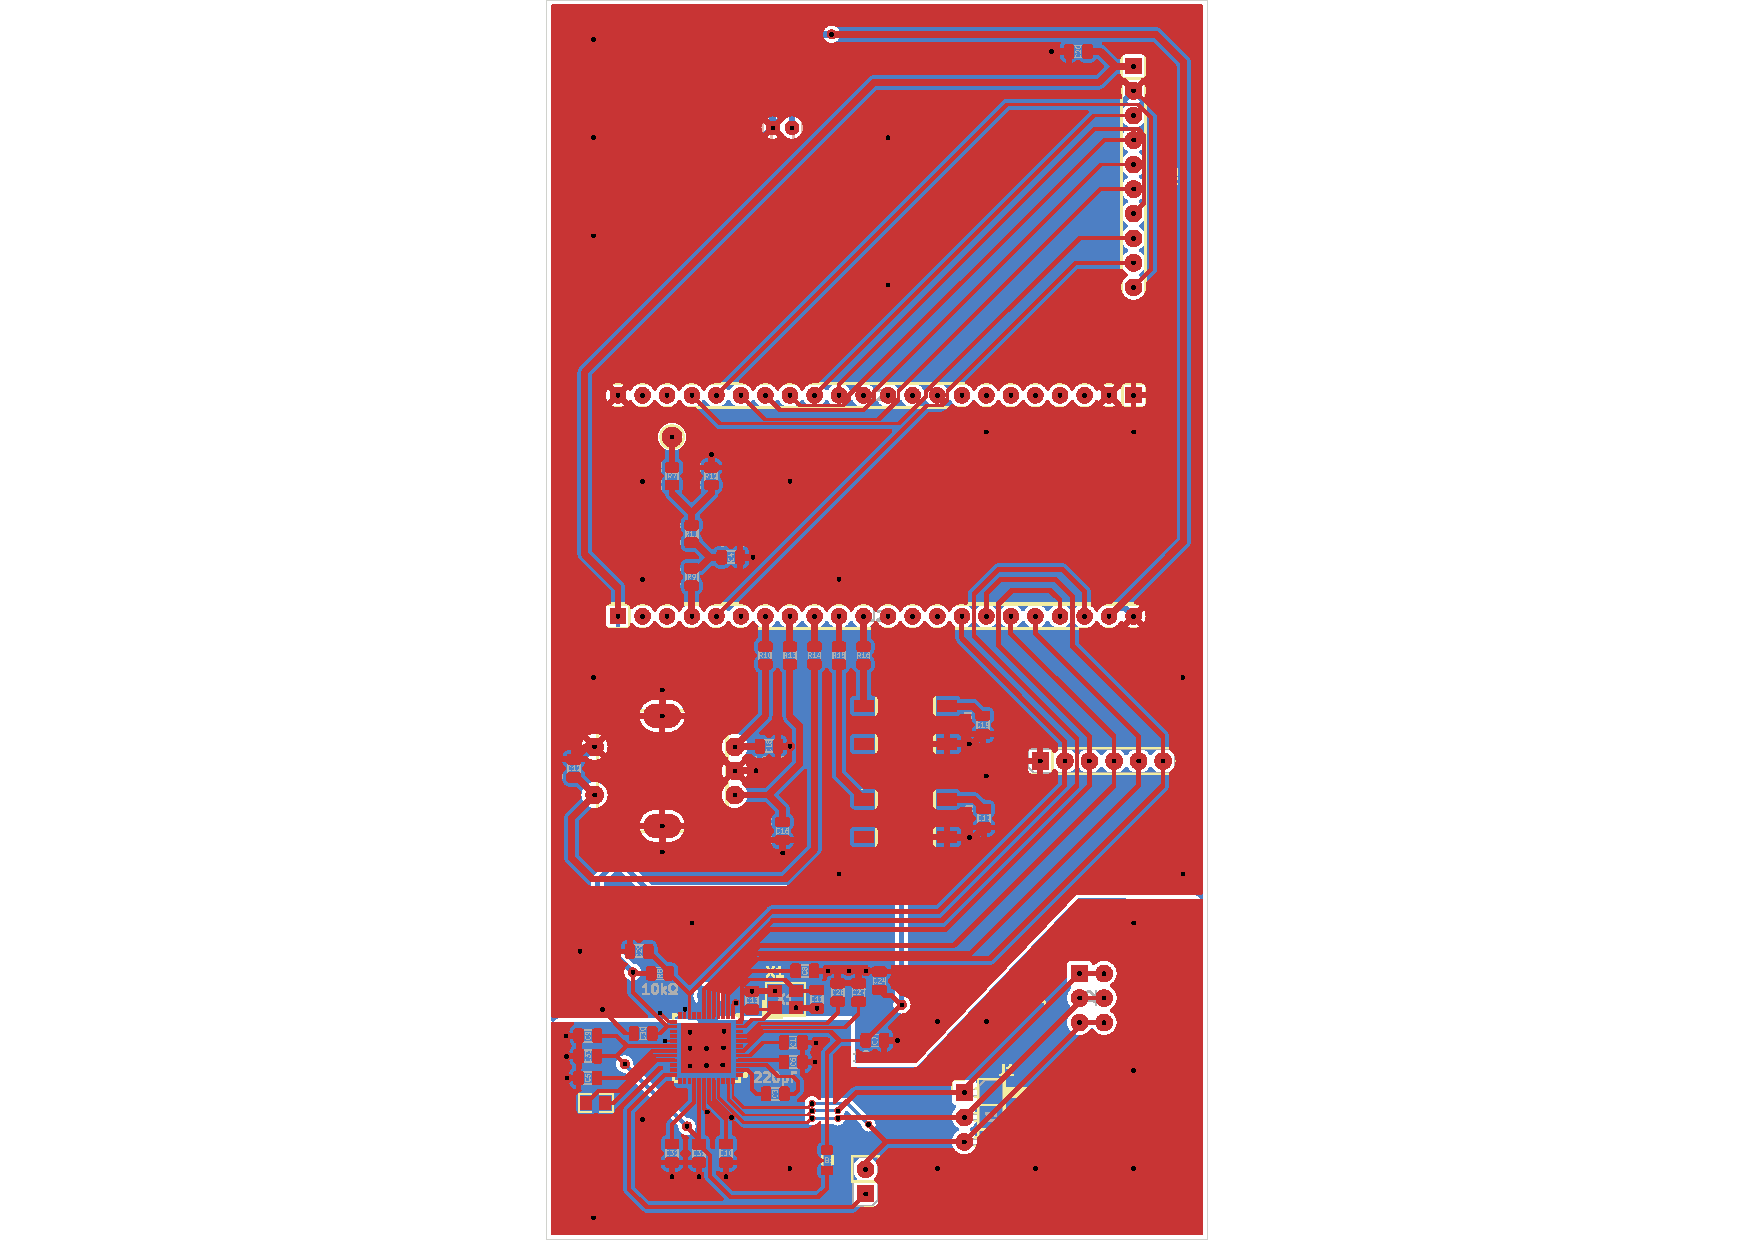
\includegraphics[trim=265 0 265 0, clip, height=6.5cm]{figures/pcbexport.pdf}
\end{wrapfigure}
To combat this, the PCB was partitioned into an analog region and a digital
region, which are the lower and upper parts of the board respectively
(Figure~\ref{fig:hw_ground_partition}), with
all digital components and traces confined to the digital region.
Partitioning is effective because, at high frequencies such as those in
digital edges, the return current follows the path of least inductance and
flows in the ground copper directly beneath its own signal trace
\cite{ott2009emc, pithadia2013grounding}. In accordance with Analog Devices guidance, the analog and digital grounds should be joined through the
shortest possible connection \cite{pithadia2013grounding, adi_mt031}. This is done by stitching them together directly beneath
the AD5941, commonly called a star ground connection \cite{adi_mt031}. The
stitched bridge also serves as the crossing point for the SPI bus and the
reset and interrupt lines, so each signal retains a continuous return path
directly underneath it. If the two grounds had been fully separated and joined
only at a distant point, such as the power input, these return currents would
be forced around a large loop that acts as an antenna \cite{ott2001partitioning}.

At the sub-nanoampere currents estimated in Section~\ref{sec:dpv_applications}, leakage and interference on the working-electrode path can set the noise floor. The electrode lead used in testing was unshielded; however, it was kept short to minimise noise pickup. A spare analog ground pin beside the electrode interface allows a shielded cable to be terminated at the interface.

\subsection{Trace Widths}
\label{sec:hw_trace_widths}

Trace widths were checked with the IPC-2221 equations \cite{ipc2221} as implemented in the DigiKey calculator \cite{digikey_tracewidth}, for a \SI{10}{\celsius} rise in 1\,oz/ft\textsuperscript{2} external copper. The \SI{0.3}{\milli\metre} traces used for the AD5941 and display nets can carry \SI{1.0}{\ampere} and the \SI{0.6}{\milli\metre} supply traces \SI{1.65}{\ampere}, well above their design currents of \SI{10}{\milli\ampere}, \SI{33}{\milli\ampere} and \SI{1}{\ampere}. See Appendix~\ref{app:trace_width} for more information.

\section{Display and SD Card}
\label{sec:hw_display}

The DFRobot Fermion 1.8-inch TFT (DFR0928) was selected as the display because it meets requirements R4–R7 from Table~\ref{tab:requirements_whole_sys}. The Fermion was the only component in stock that met all the criteria. Additional information regarding the display is given in Appendix Table~\ref{tab:hw_display_specs}.

The display and the SD card share a single SPI bus, because the ESP32-S3 has only two general-purpose SPI controllers \cite{esp32s3_wroom2_ds}. This allows a full SPI bus to be dedicated to the AD5941, so that scans are minimally affected. The cost is that the display and the SD card cannot be used at the same time. This is avoided by buffering the samples in PSRAM and writing the file
only after the scan has finished.

\section{Power Management}
\label{sec:hw_power}

The power subsystem was chosen to meet the requirements of 8-hour working day battery
life, over-voltage and under-voltage protection, and affordable components.
The chosen components are the TP4056 charger with a DW01A protection IC, the
Pololu S9V11E2F5 step-up/step-down regulator producing \SI{5}{\volt}, and a
\SI{5000}{\milli\ampere\hour}, \SI{3.7}{\volt} single-cell LiPo battery. Their
main specifications are summarised in Table~\ref{tab:hw_power_specs}.

\subsection{Battery}
\label{sec:hw_battery}

To verify that the selected \SI{5000}{\milli\ampere\hour} battery fulfils the full-day operational requirement, the system's current was measured during idle, transmission over Wi-Fi and DPV measurements. The supply current was measured by powering the PCB at \SI{5}{\volt} from a Siglent SPD3303C bench supply and reading the output current from the supply. The SPD3303C has a current
readback resolution of \SI{10}{\milli\ampere} and an accuracy of
$\pm\SI{0.5}{\percent}$
\cite{siglent_spd3303c}, that is, about $\pm\SI{21}{\milli\ampere}$ at these
currents. The board draws $\SI{100}{\milli\ampere} \pm \SI{21}{\milli\ampere}$
at idle and $\SI{160}{\milli\ampere} \pm \SI{21}{\milli\ampere}$ while
transmitting over Wi-Fi. The idle current did not change when taking a DPV measurement. Taking \SI{160}{\milli\ampere} as the worst case, the power drawn from the
battery through the regulator ($\eta_\text{reg} \approx 0.9$) is
\begin{equation}
  P_\text{bat} = \frac{\SI{5}{\volt} \times \SI{160}{\milli\ampere}}
                      {\eta_\text{reg}}
               = \frac{\SI{0.80}{\watt}}{0.9}
               \approx \SI{0.89}{\watt},
  \label{eq:hw_pbat}
\end{equation}
and the run time is
\begin{equation}
  t_\text{run} = \frac{E_\text{bat}\,\eta_\text{reg}}{V_\text{out}\,I_\text{load}}
    = \frac{\SI{5}{\ampere\hour} \times \SI{3.7}{\volt} \times 0.9}
           {\SI{5}{\volt} \times \SI{160}{\milli\ampere}}
    \approx \SI{21}{\hour}.
  \label{eq:hw_runtime}
\end{equation}
Allowing for the measurement uncertainty, the run time with Wi-Fi
transmitting lies between \SI{18}{\hour} and \SI{24}{\hour}, and at idle
between \SI{28}{\hour} and \SI{42}{\hour}. Even the lower bound comfortably
meets R12, as well as R9--R11.

\subsection{Charging}
\label{sec:hw_charging}

The TP4056 is a linear constant-current, constant-voltage charger with a
\SI{4.2}{\volt} float voltage, which charges at up to \SI{1}{\ampere} \cite{tp4056_ds}. A full charge of the \SI{5000}{\milli\ampere\hour} cell was measured to take about \SI{6.5}{\hour}, longer than the \SI{5}{\hour} that capacity divided by current suggests, because the charger reduces the current in its final constant-voltage stage.

\subsection{Regulation}
\label{sec:hw_regulation}

The Pololu S9V11E2F5 covers the full battery voltage range with sufficient
output current, but it requires the addition of an external low-voltage
cutoff. An MT3608 boost converter was also considered, but was rejected after three of the modules tested proved faulty. The Pololu's \SI{700}{\milli\ampere} start-up current limit is sufficient for
the ESP32-S3 to boot, and its soft-start ramps the output up gradually
\cite{pololu_s9v11e2f5}. The regulator has a \SI{100}{\kilo\ohm} pull-up
resistor from its enable pin to $V_\text{IN}$; the enable pin turns the
regulator off below \SI{0.7}{\volt} and on above \SI{0.8}{\volt}
\cite{pololu_s9v11e2f5}. Connecting a \SI{33}{\kilo\ohm} resistor from the
enable pin to ground forms a divider that switches the regulator off at about \SI{2.8}{\volt}, as given in Equation~\eqref{eq:hw_cutoff}.

The divider draws about \SI{28}{\micro\ampere} continuously, which is
sufficiently low for this application.
\begin{equation}
  V_\text{off} = \SI{0.7}{\volt} \times
    \frac{\SI{100}{\kilo\ohm} + \SI{33}{\kilo\ohm}}{\SI{33}{\kilo\ohm}}
    \approx \SI{2.8}{\volt}
  \label{eq:hw_cutoff}
\end{equation}

The \SI{5}{\volt} output supplies the ESP32-S3 development board, whose on-board regulator provides the \SI{3.3}{\volt} rail for the whole PCB, including AVDD of the AD5941.
% CHECK: confirm this matches your board; if the 3.3 V comes from a regulator on your own PCB, name that part instead.
A design oversight was the choice to boost the voltage to \SI{5}{\volt} when
no component requires a \SI{5}{\volt} supply. A \SI{3.3}{\volt}
step-up/step-down regulator would have been more efficient. The large
\SI{5000}{\milli\ampere\hour} battery makes this loss affordable, although it
is not ideal.

\subsection{Input Decoupling}
\label{sec:hw_input_decoupling}

No single capacitor has a low impedance across the whole frequency range, so a
large capacitor for low frequencies is paired with a small one for high
frequencies \cite{adi_mt101}. Decoupling is required because high-frequency
noise couples through to the regulator output and must be kept out of the chip
\cite{adi_mt101}. A \SI{100}{\micro\farad} bulk capacitor is used at the
output of the boost regulator, which is the input to the PCB, to act as a
local charge reservoir. An additional \SI{100}{\nano\farad} capacitor shunts
high-frequency noise away from the PCB \cite{adi_mt101}.

\section{User Interface}
\label{sec:hw_ui}

The interface consists of two push buttons and a rotary encoder with an integrated push button. All are wired in an active-low configuration with \SI{10}{\kilo\ohm} hardware pull-up resistors. A capacitor on each line forms an RC filter with its pull-up, so on release the pin only reads high once the capacitor has charged past the ESP32-S3 input-high threshold of $0.75 \times V_{DD}$ \cite{esp32s3_ds}. This takes $t = RC\ln 4 \approx 1.39\,RC$.

The push buttons use \SI{100}{\nano\farad} (\SI{1.4}{\milli\second}) to absorb contact bounce \cite{allpcb_debounce}, and the encoder lines use \SI{10}{\nano\farad} (\SI{0.14}{\milli\second}) so that fast rotation is not smeared; the remaining encoder bounce, which can last up to \SI{2}{\milli\second} \cite{alps_ec11}, is rejected by the quadrature decoder in firmware.

The OpenStat has two user interfaces, shown in Figure~\ref{fig:interface}. On the device, the rotary encoder selects and edits the scan parameters of Table~\ref{tab:sw_params}, the push buttons start and stop a scan, and the display shows the voltammogram as it is measured. The web interface offers the same parameters, a live voltammogram and a list of stored scans that can be downloaded. If the device cannot join a known Wi-Fi network, it starts its own access point, so that a phone or laptop can connect to it in the field (Section~\ref{sec:sw_toplevel}).

\begin{figure}[htbp]
  \centering
  \caption{OpenStat user interfaces. (a) Physical interface, shown connected to the Randles test circuits. (b) Web interface displaying a live voltammogram.}
  \label{fig:interface}
  \begin{minipage}[b]{0.38\textwidth}
    \centering
    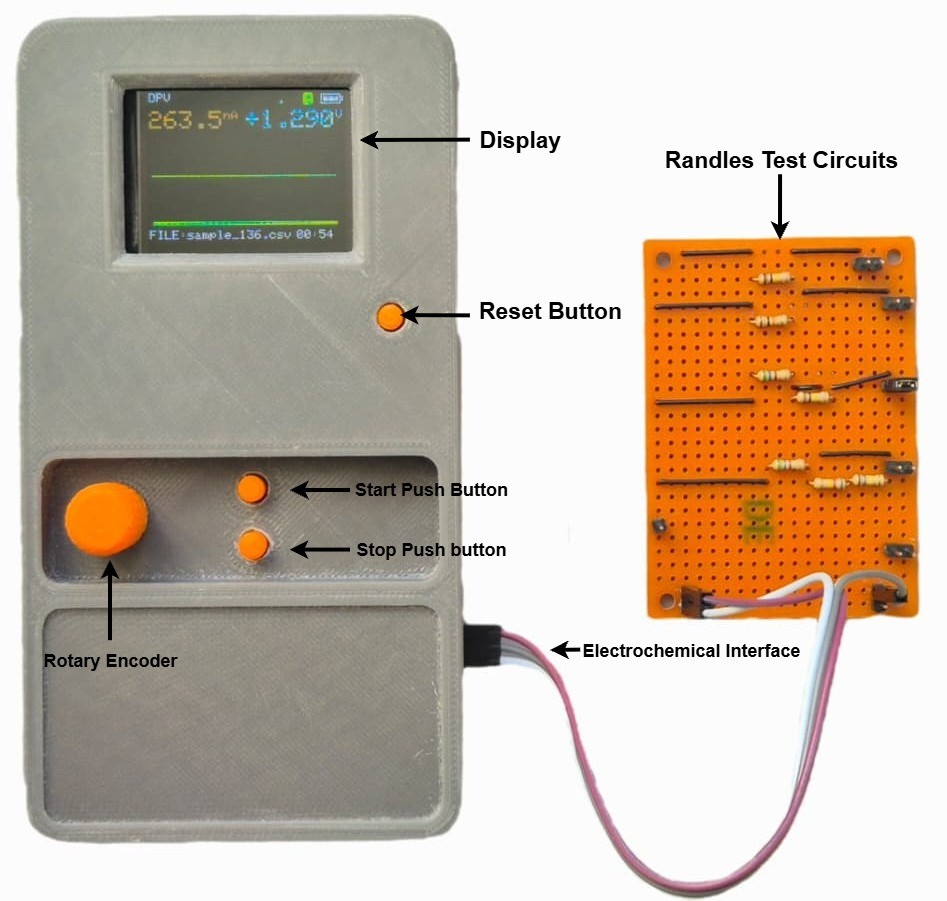
\includegraphics[width=\linewidth]{figures/sweep_136_lab.jpg}\\
    (a)
  \end{minipage}
  \hfill
  \begin{minipage}[b]{0.58\textwidth}
    \centering
    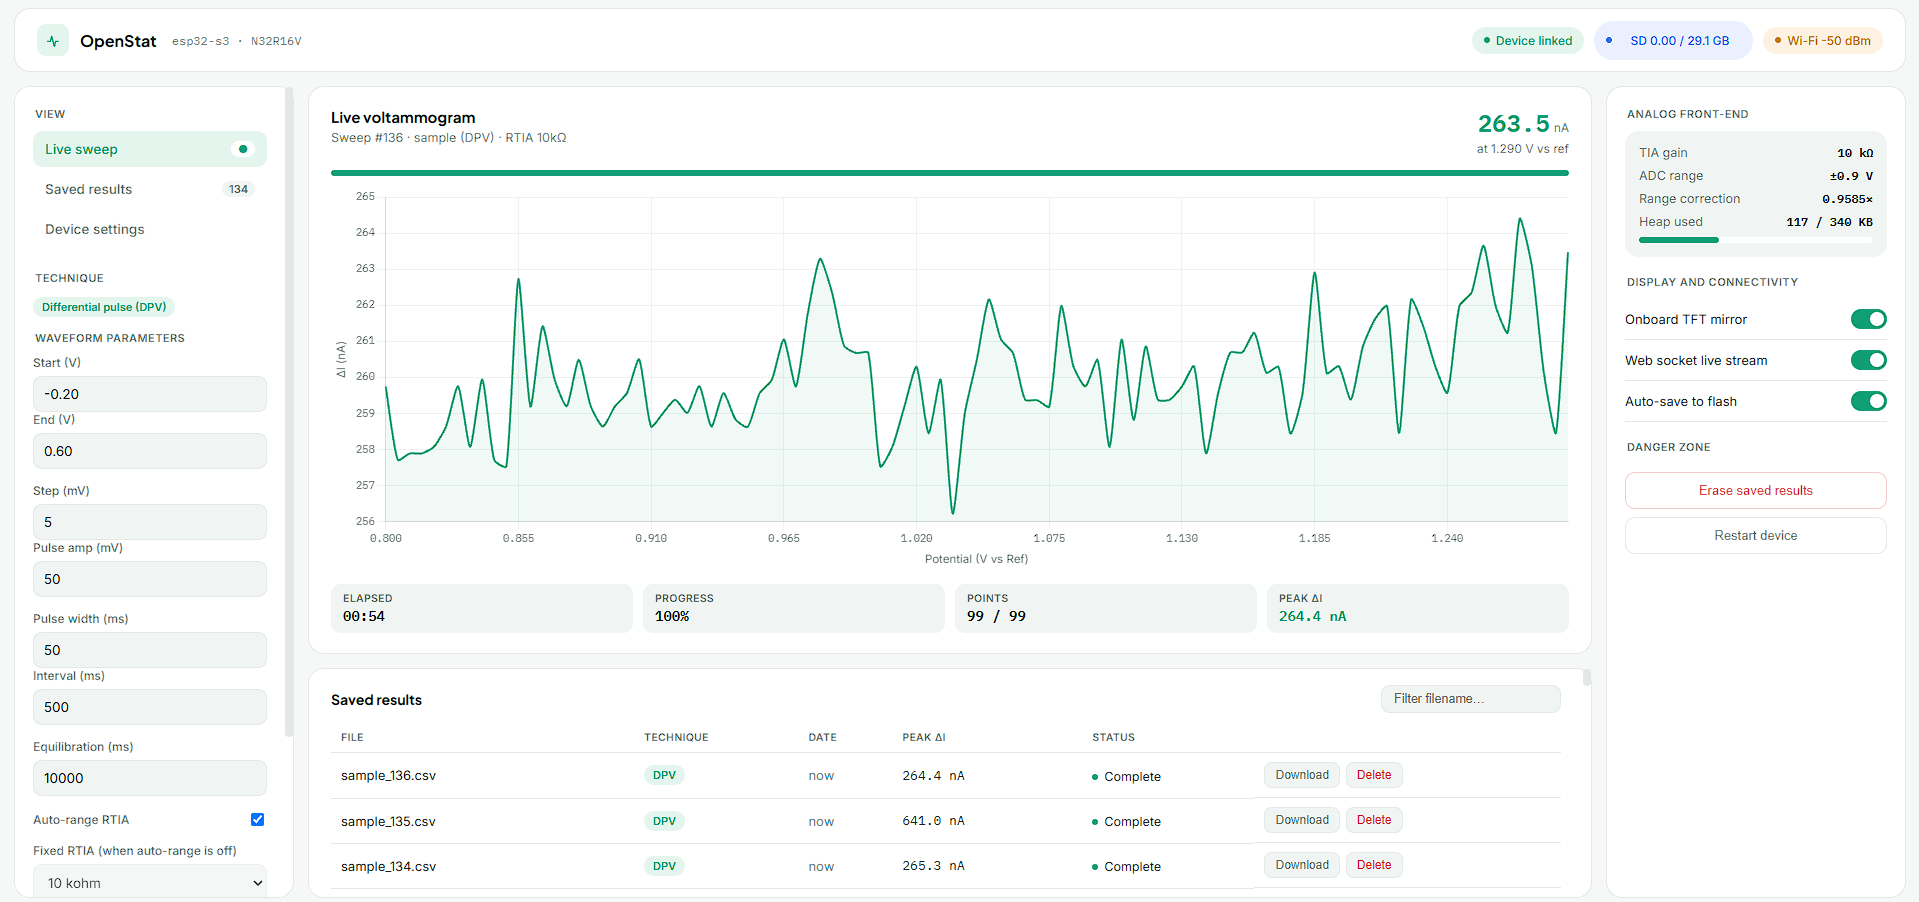
\includegraphics[width=\linewidth]{figures/sweep136.png}\\
    (b)
  \end{minipage}
\end{figure}
\usetikzlibrary{arrows.meta, positioning, calc, shapes.geometric, fit, patterns}

\tikzset{
  swbase/.style={draw, align=center, font=\footnotesize, inner sep=3pt,
                 line width=0.5pt,
                 execute at begin node={\hyphenpenalty=10000\relax\exhyphenpenalty=10000\relax}},
  swproc/.style={swbase, rectangle, minimum height=7mm, text width=#1},
  swproc/.default=34mm,
  swterm/.style={swbase, rectangle, rounded corners=3.4mm,
                 minimum height=7mm, text width=#1},
  swterm/.default=30mm,
  swdec/.style={swbase, diamond, aspect=2.4, inner sep=0.5pt, text width=#1},
  swdec/.default=24mm,
  % predefined process (detailed in another figure): box with side bars
  swsub/.style={swproc=#1, inner xsep=4.5mm,
    path picture={
      \draw[line width=0.5pt]
        ([xshift=1.6mm]path picture bounding box.north west) --
        ([xshift=1.6mm]path picture bounding box.south west)
        ([xshift=-1.6mm]path picture bounding box.north east) --
        ([xshift=-1.6mm]path picture bounding box.south east);}},
  swsub/.default=30mm,
  swarr/.style={-{Latex[length=2mm]}, line width=0.5pt},
  swdbl/.style={{Latex[length=2mm]}-{Latex[length=2mm]}, line width=0.5pt},
  swlbl/.style={font=\scriptsize, inner sep=1.5pt},
  swhw/.style={swbase, rectangle, minimum height=8mm, text width=#1,
               fill=black!10},
  swhw/.default=26mm,
}

\providecommand{\swtodo}[1]{\textbf{[TODO: #1]}}

\usetikzlibrary{arrows.meta, positioning, calc, shapes.geometric, fit, patterns}

\tikzset{
  swbase/.style={draw, align=center, font=\footnotesize, inner sep=3pt,
                 line width=0.5pt,
                 execute at begin node={\hyphenpenalty=10000\relax\exhyphenpenalty=10000\relax}},
  swproc/.style={swbase, rectangle, minimum height=7mm, text width=#1},
  swproc/.default=34mm,
  swterm/.style={swbase, rectangle, rounded corners=3.4mm,
                 minimum height=7mm, text width=#1},
  swterm/.default=30mm,
  swdec/.style={swbase, diamond, aspect=2.4, inner sep=0.5pt, text width=#1},
  swdec/.default=24mm,
  % predefined process (detailed in another figure): box with side bars
  swsub/.style={swproc=#1, inner xsep=4.5mm,
    path picture={
      \draw[line width=0.5pt]
        ([xshift=1.6mm]path picture bounding box.north west) --
        ([xshift=1.6mm]path picture bounding box.south west)
        ([xshift=-1.6mm]path picture bounding box.north east) --
        ([xshift=-1.6mm]path picture bounding box.south east);}},
  swsub/.default=30mm,
  swarr/.style={-{Latex[length=2mm]}, line width=0.5pt},
  swdbl/.style={{Latex[length=2mm]}-{Latex[length=2mm]}, line width=0.5pt},
  swlbl/.style={font=\scriptsize, inner sep=1.5pt},
  swhw/.style={swbase, rectangle, minimum height=8mm, text width=#1,
               fill=black!10},
  swhw/.default=26mm,
}

\chapter{Software Design}
\label{chap:software_design}

The hardware described in Chapter~\ref{chap:hardware_design} has the ability to apply a
potential to the cell and measure the current that flows, but it is the
firmware that turns these two features into a useful measurement.
This chapter describes the structure of the firmware and the logic of how a measurement is performed.

% The firmware has four tasks; to generate the DPV waveform, to sample and convert the cell current, to store the result, and to present it to the user.


\begin{figure}[H]
  \centering
  \caption{Software structure.
    Arrows show the direction of calls or data.}
  \label{fig:architecture}
  \begin{tikzpicture}[x=1cm, y=1cm]
    % --- external, top
    \node[swhw=30mm] (browser) at (7.6, 6.9) {Browser dashboard};
    \node[swhw=26mm] (pc)      at (12.8, 6.9) {Serial terminal};
    % --- row A
    \node[swproc=36mm] (screens) at (2.3, 5.0) {Screens and screen\\state machine};
    \node[swproc=34mm] (web)     at (7.6, 5.0) {Web server\\(HTTP, WebSocket)};
    \node[swproc=26mm] (serial)  at (12.8, 5.0) {Serial bench\\commands};
    % --- row B
    \node[swproc=16mm] (input)  at (0.5, 3.0) {Input\\manager};
    \node[swproc=46mm, minimum height=10mm] (engine) at (7.6, 3.0)
      {\textbf{Sweep engine}\\result buffer and storage};
    \node[swproc=26mm] (params) at (12.8, 3.0) {Scan parameters\\(saved in NVS)};
    % --- row C
    \node[swproc=22mm] (render) at (3.1, 1.0) {Renderer};
    \node[swproc=26mm] (driver) at (12.0, 1.0) {AD5941 driver};
    % --- firmware boundary
    \node[draw, dashed, line width=0.5pt, inner sep=3mm,
          fit=(screens)(serial)(input)(render)(driver)(params)] (fw) {};
    \node[swlbl, anchor=south west, font=\footnotesize\itshape]
      at ([yshift=0.3mm]fw.north west) {ESP32-S3 firmware};
    % --- hardware, bottom
    \node[swhw=16mm] (enc)  at (0.5, -1.1) {Encoder,\\buttons};
    \node[swhw=22mm] (tft)  at (3.1, -1.1) {TFT display};
    \node[swhw=24mm] (sd)   at (7.6, -1.1) {microSD card};
    \node[swhw=26mm] (afe)  at (12.0, -1.1) {AD5941 AFE};
    % --- connections
    \draw[swdbl] (browser) -- node[swlbl, right] {Wi-Fi} (web);
    \draw[swdbl] (pc) -- node[swlbl, right] {USB} (serial);
    \draw[swarr] (enc) -- node[swlbl, right, align=left, pos=0.12] {GPIO,\\interrupts} (input);
    \draw[swarr] (input.north) -- node[swlbl, left] {events}
      (input.north |- screens.south);
    \draw[swarr] ([xshift=-4mm]render.north |- screens.south) --
      node[swlbl, left, pos=0.3] {draw} ([xshift=-4mm]render.north);
    \draw[swdbl] ([xshift=16mm]screens.south) |-
      node[swlbl, right, pos=0.22] {callbacks} (engine.west);
    \draw[swarr] ([xshift=-17mm]engine.south) |-
      node[swlbl, above, pos=0.75] {live trace} (render.east);
    \draw[swdbl] (web) -- node[swlbl, left] {commands, points} (engine);
    \draw[swarr] (serial.south) -- ++(0,-0.5) -| ([xshift=17mm]engine.north);
    \draw[swdbl] (params) -- (engine);
    \draw[swarr] ([xshift=17mm]engine.south) |- (driver.west);
    \draw[swarr] (render) -- node[swlbl, right, pos=0.72] {SPI (HSPI)} (tft);
    \draw[swdbl] (engine) -- node[swlbl, right, pos=0.86] {SPI (HSPI)} (sd);
    \draw[swdbl] (driver) --
      node[swlbl, right, align=left, pos=0.72] {SPI (FSPI),\\\SI{4}{\mega\hertz}} (afe);
  \end{tikzpicture}
\end{figure}

Each of the modules in Figure~\ref{fig:architecture} is described in the sections that follow.

\section{Software Overview}
\label{sec:sw_overview}

The firmware is written in C++ on the Arduino framework for the ESP32-S3 and
is built with PlatformIO. Third-party libraries like Adafruit GFX and ST7735 are used for the display, ESPAsyncWebServer and AsyncTCP for
the web server and ArduinoJson for JSON encoding.


There were three design decisions shaped the structure of the software:
\begin{itemize}[label=\textbullet]
  \item \textbf{Project-specific AD5941 driver.} Analog Devices
    supplies a general-purpose software library for the AFE, which covers every measurement mode of the device. The driver for this project was adapted from this library and was written around the needs of this project. This gives
    the firmware direct control of the gain resistor $R_\text{TIA}$ of the
    transimpedance amplifier, which the automatic range selection in
    Section~\ref{sec:sw_ranging} switches repeatedly before a scan.

  \item \textbf{One sweep engine, two front ends.} The on-device screens and
    the web dashboard both start, stop and observe a measurement through the
    same sweep engine, so a scan behaves identically regardless of the interface that started the sweep.
  \item \textbf{A dedicated SPI bus for the AFE.} The display and the SD card
    share an SPI bus so
    display and storage traffic never occupies the bus used for the
    measurement.
\end{itemize}


% \begin{figure}[H]
%   \centering
%   \begin{tikzpicture}[x=1cm, y=1cm]
%     % --- external, top
%     \node[swhw=30mm] (browser) at (7.6, 6.9) {Browser dashboard};
%     \node[swhw=26mm] (pc)      at (12.8, 6.9) {Serial terminal};
%     % --- row A
%     \node[swproc=36mm] (screens) at (2.3, 5.0) {Screens and screen\\state machine};
%     \node[swproc=34mm] (web)     at (7.6, 5.0) {Web server\\(HTTP, WebSocket)};
%     \node[swproc=26mm] (serial)  at (12.8, 5.0) {Serial bench\\commands};
%     % --- row B
%     \node[swproc=16mm] (input)  at (0.5, 3.0) {Input\\manager};
%     \node[swproc=46mm, minimum height=10mm] (engine) at (7.6, 3.0)
%       {\textbf{Sweep engine}\\result buffer and storage};
%     \node[swproc=26mm] (params) at (12.8, 3.0) {Scan parameters\\(saved in NVS)};
%     % --- row C
%     \node[swproc=22mm] (render) at (3.1, 1.0) {Renderer};
%     \node[swproc=26mm] (driver) at (12.0, 1.0) {AD5941 driver};
%     % --- firmware boundary
%     \node[draw, dashed, line width=0.5pt, inner sep=3mm,
%           fit=(screens)(serial)(input)(render)(driver)(params)] (fw) {};
%     \node[swlbl, anchor=south west, font=\footnotesize\itshape]
%       at ([yshift=0.3mm]fw.north west) {ESP32-S3 firmware};
%     % --- hardware, bottom
%     \node[swhw=16mm] (enc)  at (0.5, -1.9) {Encoder,\\buttons};
%     \node[swhw=22mm] (tft)  at (3.1, -1.9) {TFT display};
%     \node[swhw=24mm] (sd)   at (7.6, -1.9) {microSD card};
%     \node[swhw=26mm] (afe)  at (12.0, -1.9) {AD5941 AFE};
%     % --- connections
%     \draw[swdbl] (browser) -- node[swlbl, right] {Wi-Fi} (web);
%     \draw[swdbl] (pc) -- node[swlbl, right] {USB} (serial);
%     \draw[swarr] (enc) -- node[swlbl, right, align=left, pos=0.2] {GPIO,\\interrupts} (input);
%     \draw[swarr] (input.north) -- node[swlbl, left] {events}
%       (input.north |- screens.south);
%     \draw[swarr] ([xshift=-4mm]render.north |- screens.south) --
%       node[swlbl, left, pos=0.3] {draw} ([xshift=-4mm]render.north);
%     \draw[swdbl] ([xshift=16mm]screens.south) |-
%       node[swlbl, right, pos=0.22] {callbacks} (engine.west);
%     \draw[swarr] ([xshift=-17mm]engine.south) |-
%       node[swlbl, above, pos=0.75] {live trace} (render.east);
%     \draw[swdbl] (web) -- node[swlbl, left] {commands, points} (engine);
%     \draw[swarr] (serial.south) -- ++(0,-0.5) -| ([xshift=17mm]engine.north);
%     \draw[swdbl] (params) -- (engine);
%     \draw[swarr] ([xshift=17mm]engine.south) |- (driver.west);
%     \draw[swarr] (render) -- node[swlbl, right, pos=0.72] {SPI (HSPI)} (tft);
%     \draw[swdbl] (engine) -- node[swlbl, right, pos=0.86] {SPI (HSPI)} (sd);
%     \draw[swdbl] (driver) --
%       node[swlbl, right, align=left, pos=0.72] {SPI (FSPI),\\\SI{4}{\mega\hertz}} (afe);
%   \end{tikzpicture}
%   \caption{Software architecture.
%     Arrows show the direction of calls or data.}
%   \label{fig:sw_architecture}
% \end{figure}

The dedicated bus keeps display and storage traffic away from the measurement
in hardware, but all of these modules still share the processor's time. How
that time is divided, and when the measurement takes priority, is set by the
top-level program flow.

\section{Top-Level Program Flow}  
\label{sec:sw_toplevel}

All project code runs from a single loop, shown in
Figure~\ref{fig:sw_toplevel}. During boot-up the device does a check to see if the WiFi, SD card  and AD5941 is working correctly, after these checks are done the user is taken into the home display. The state of the device is stored in three places, the active screen, a flag that records whether a scan is running, and the phase of the DPV step inside the AFE driver. The loop services each of these in turn on
every pass and none of them blocks the loop, except when the device is sampling which is discussed in Section~\ref{sec:sw_sampling}.

\begin{figure}[!htb]
  \centering
  \caption{Top-level program flow: start-up sequence (left) and the
    cooperative main loop (right).}
  \label{fig:sw_toplevel}
  \begin{tikzpicture}[node distance=4.5mm and 12mm]
    % --- start-up column
    \node[swterm=22mm] (pwr) {Power on};
    \node[swproc=42mm, below=of pwr] (disp) {Serial port, display and\\splash screen};
    \node[swproc=42mm, below=of disp] (nvs) {Load scan parameters from\\NVS and clamp to limits};
    \node[swproc=42mm, below=of nvs] (wifi) {Connect to Wi-Fi; on timeout\\start access point};
    \node[swproc=42mm, below=of wifi] (afe) {Reset AD5941, check ID,\\write configuration};
    \node[swproc=42mm, below=of afe] (sd) {Mount SD card, load\\results index};
    \node[swproc=42mm, below=of sd] (ui) {Start inputs, screens (Boot\\screen) and web server};
    \foreach \a/\b in {pwr/disp, disp/nvs, nvs/wifi, wifi/afe, afe/sd, sd/ui}
      \draw[swarr] (\a) -- (\b);
    % --- loop column
    \node[swproc=46mm, right=22mm of disp] (l1) {Read inputs; pass events\\to the active screen};
    \node[swproc=46mm, below=of l1] (l2) {Update the active screen};
    \node[swproc=46mm, below=of l2] (l3) {Handle serial commands};
    \node[swsub=38mm, below=of l3] (l4) {Service the scan\\(Figure~\ref{fig:sw_scan})};
    \node[swdec=24mm, below=of l4] (l5) {Scan\\running?};
    \node[swproc=46mm, below=of l5] (l6) {Send status to dashboard\\every \SI{2}{\second}};
    \foreach \a/\b in {l1/l2, l2/l3, l3/l4, l4/l5}
      \draw[swarr] (\a) -- (\b);
    \draw[swarr] (l5) -- node[swlbl, right] {no} (l6);
    \coordinate (lb) at ($(l6.south)+(3.3,-0.4)$);
    \draw[swarr] (l6.south) -- ++(0,-0.4) -- (lb) |- (l1.east);
    \draw[line width=0.5pt] (l5.east) -- node[swlbl, above, pos=0.3] {yes} (l5.east -| lb);
    \fill (l5.east -| lb) circle (1.1pt);
    \draw[swarr] (ui.east) -- ++(0.75,0) |- (l1.west);
    \node[swlbl, anchor=south, font=\footnotesize\itshape] at ([yshift=1mm]l1.north) {main loop};
    \node[swlbl, anchor=south, font=\footnotesize\itshape] at ([yshift=1mm]pwr.north) {start-up};
  \end{tikzpicture}
\end{figure}

% ---------------------------------------------------------------------
\section{DPV Measurement Sequence}
\label{sec:sw_dpv}

A scan is defined by the parameters required in Table~\ref{tab:sw_params}. They are
stored in non-volatile storage (NVS), a partition of the ESP's flash memory, edited on the device and restricted to the limits seen in Table~\ref{tab:sw_ranges} whenever they are loaded or edited to protect the hardware. The scan rate is not set directly and is found by dividing the number of steps by the period.

\begin{table}[H]
  \centering
  \small
  \caption{DPV scan parameters, their default values and permitted ranges.}
  \label{tab:sw_params}
  \begin{tabular}{@{}llll@{}}
    \toprule
    \textbf{Parameter} & \textbf{Symbol} & \textbf{Default} & \textbf{Permitted range} \\
    \midrule
    Start potential   & $E_\text{start}$    & \SI{0.80}{\volt}        & \SI{-0.35}{\volt} to $E_\text{end} - \Delta E_\text{s}$ \\
    End potential     & $E_\text{end}$      & \SI{1.30}{\volt}        & $E_\text{start} + \Delta E_\text{s}$ to \SI{1.30}{\volt} \\
    Step              & $\Delta E_\text{s}$ & \SI{5}{\milli\volt}     & \SIrange{1}{50}{\milli\volt} \\
    Pulse amplitude   & $\Delta E_\text{p}$ & \SI{25}{\milli\volt}    & \SIrange{-100}{100}{\milli\volt} \\
    Pulse width       & $t_\text{p}$        & \SI{50}{\milli\second}  & \SIrange{10}{500}{\milli\second} \\
    Pulse period      & $T$                 & \SI{500}{\milli\second} & \SIrange{50}{5000}{\milli\second} \\
    TIA range         & $R_\text{TIA}$      & automatic               & automatic, or one of eight fixed values \\
    \bottomrule
  \end{tabular}
\end{table}

\subsection{Generating the Potential}
\label{sec:sw_potential}

The cell potential is set by the two outputs of the low-power DAC of the
AD5941. The 6-bit output $V_\text{ZERO}$ biases the high-speed transimpedance
amplifier (TIA), which holds the working electrode at that voltage, and is
fixed at \SI{1.7125}{\volt}. The 12-bit output $V_\text{BIAS}$ drives
the reference electrode through the potentiostat amplifier and carries the
staircase and the pulses. 

The applied potential is therefore
\begin{equation}
  E = V_\text{ZERO} - V_\text{BIAS}, where
  \qquad
  V_\text{BIAS} = \SI{0.2}{\volt} + D_{12}\times\frac{\SI{2.2}{\volt}}{4095},
  \label{eq:sw_potential}
\end{equation}
and $D_{12}$ is the 12-bit code and one code is \SI{537.2}{\micro\volt} which represents the voltage change per code. With
$V_\text{ZERO}$ fixed at this value, the permitted range of $E$ in
Table~\ref{tab:sw_params} keeps $V_\text{BIAS}$ between \SI{0.41}{\volt} and
\SI{2.06}{\volt}, inside the \SIrange{0.2}{2.4}{\volt} output range of the DAC.

\subsection{Scan Flow}

Before any timing starts, the TIA range is selected (Section~\ref{sec:sw_ranging}) and the requested timing is checked against the minimum that the sampling scheme can support
(Section~\ref{sec:sw_sampling}), a scan that fails this check is stopped. The scan consists of
\begin{equation}
  N = \left\lfloor \frac{E_\text{end} - E_\text{start}}{\Delta E_\text{s}} \right\rfloor
  \label{eq:sw_npoints}
\end{equation}
% CHECK: for the defaults this is 100 on paper, but the firmware evaluates it
% in single-precision floating point and (by the summary's arithmetic) gets
% 99. Confirm against the serial line "Sweep state: RUNNING (DPV, N points".
points, and the end potential itself is not applied as a base level. Each
point is produced by the step routine in Figure~\ref{fig:sw_step}, which the
main loop calls on every pass. The routine returns immediately unless a
sampling window is due, so the user interface stays responsive during the
\SI{450}{\milli\second} base dwell.

Points are held in memory during the scan and written to the SD card as a
single file only once the scan has stopped, so that card activity cannot
disturb the measurement. Every way of leaving a scan, whether completion, a
stop request or an overload, passes through the same stop routine, which stops
the ADC, returns the cell to $E = \SI{0}{\volt}$ and saves the points captured
so far. For more detail Figure~\ref{fig:sw_scan} in Appendix~\ref{app:scan_flow_timing} shows the process of how one scan is run. 


\section{Pulse Sampling and Timing}
\label{sec:sw_sampling}

DPV rejects the capacitive charging current only if $I_\text{before}$ and
$I_\text{end}$ are each sampled after the transient from the preceding edge
has decayed, as shown in Section~\ref{sec:dpv_rejection}. When the current is sampled, and for how long, therefore sets both
the noise of the measurement and how much charging current leaks into
$\Delta I$.

\subsection{Software Timing}
\label{sec:sw_timing}

All DAC updates and ADC conversions are done on the microcontroller. The staircase and the pulses are individual DAC writes over SPI, scheduled by the ESP32-S3 against its millisecond clock, and data-ready is detected by polling the interrupt flag register of the AD5941. This was a deliberate choice: timing the measurement in firmware gives the ESP32-S3 full control over when every operation in the system takes place, so the measurement can be scheduled around the display, storage and network activity instead of running alongside it.

That control is used to give the measurement priority over everything else
while a scan is running. Whenever the current is being sampled, the firmware
does nothing but sample: the buttons are not read, the display is not
updated and nothing is written to the SD card. This keeps the
digital activity of the device out of the sampling windows, which reduces the
noise coupled into the measurement and improves its accuracy. The cost is
that the timing between windows depends on the main loop, and the sampling
scheme below was designed so that this dependence does not reach the measured
current.

\subsection{Averaging Window}
\label{sec:sw_window}

The AD5941 has an analog path that has to be wide so that the cell current is converted faithfully as it changes at each pulse edge. The HSTIA is specified  for signals up to \SI{200}{\kilo\hertz} \cite[p.~50]{ad5941_ds}. Before the ADC of the AD5941 transmits the measurements to the ESP32-S3 its output
passes through two digital filters inside the device, a sinc3 filter
followed by a sinc2 filter \cite[p.~57]{ad5941_ds}. A sinc filter is a
low-pass filter that averages a block of consecutive samples and outputs
one result per block, so it both suppresses noise and lowers the data rate.
The number of samples per output is the oversampling ratio. In the
configuration used, the sinc3 filter reduces the raw \SI{800}{\kilo\hertz}
ADC rate by a factor of 5 to \SI{160}{\kilo\hertz}, and the sinc2 filter
reduces it further by a factor of 178 \cite[p.~59]{ad5941_ds}, resulting in an effective sampling frequency of \SI{900}{\hertz}. The digital bandwidths of the sinc3 filter is about \SI{42}{\kilo\hertz} and the sinc2 filter is \SI{290}{\hertz} The device also offers a
\SI{50}{\hertz}/\SI{60}{\hertz} notch filter after the sinc2 filter, but with
it enabled the settling time after a step is \SI{37}{\milli\second}, against
\SI{2.245}{\milli\second} without it \cite[p.~17]{ad5941_ds}. A
\SI{37}{\milli\second} settling time would consume most of a
\SI{50}{\milli\second} pulse, so the notch filter is bypassed and mains
rejection is provided in firmware instead: each current value is the mean of
$N_\text{w} = 18$ consecutive sinc2 results. The window length is
\begin{equation}
  T_\text{w} = N_\text{w} T_\text{s} = 18 \times \SI{1.1125}{\milli\second}
             = \SI{20.025}{\milli\second},
  \label{eq:sw_window}
\end{equation}
which is one period of the \SI{50}{\hertz} mains to within
\SI{0.13}{\percent}. This places zeros at multiples of 49.95Hz creating an effective filter. The window is defined by a sample count and not by a
duration, so every window in a scan has exactly the same length, and the ADC
runs continuously for the whole scan so that the filters are never restarted
between windows.

\subsection{Placing Windows}

Figure~\ref{fig:sw_timing} shows where the two windows fall within a step.
Each window starts \SI{21}{\milli\second} before the edge that follows it,
so that it ends at the edge: $I_\text{before}$ is the mean current over the
last \SI{20}{\milli\second} of the base dwell and $I_\text{end}$ the mean over
the last \SI{20}{\milli\second} of the pulse. These are the points of each
phase at which the charging current has had the longest time to decay.

\begin{figure}[!htb]
  \centering
  \caption{One DPV step with the default timing. Shaded bands show the two averaging windows.}
  \label{fig:sw_timing}
  \begin{tikzpicture}[x=0.94cm, y=1cm, font=\footnotesize]
    % sampling windows
    \fill[black!18] (4.6,0.2) rectangle (6.0,3.45);
    \fill[black!18] (6.8,0.2) rectangle (8.2,3.45);
    \node[swlbl, font=\footnotesize] at (5.3,3.68) {$I_\text{before}$};
    \node[swlbl, font=\footnotesize] at (7.5,3.68) {$I_\text{end}$};
    % waveform
    \draw[line width=0.9pt]
      (-1.3,2.1) -- (0,2.1) -- (0,1.0) -- (6.0,1.0) -- (6.0,2.6) -- (8.2,2.6)
      -- (8.2,1.5) -- (12.6,1.5);
    \draw[densely dotted] (12.6,1.5) -- (13.2,1.5);
    \draw[densely dotted] (-1.3,2.1) -- (-1.8,2.1);
    % axes
    \draw[-{Latex[length=2mm]}] (-1.8,0.2) -- (13.6,0.2) node[below left] {time};
    \draw[-{Latex[length=2mm]}] (-1.8,0.2) -- (-1.8,3.75) node[above] {$E$};
    % amplitude dimensions
    \draw[densely dashed, line width=0.3pt] (6.0,1.0) -- (11.2,1.0);
    \draw[{Latex[length=1.5mm]}-{Latex[length=1.5mm]}] (10.9,1.0) --
      node[right, inner sep=2pt] {$\Delta E_\text{s}$} (10.9,1.5);
    \draw[densely dashed, line width=0.3pt] (8.2,2.6) -- (9.6,2.6);
    \draw[{Latex[length=1.5mm]}-{Latex[length=1.5mm]}] (9.3,1.0) --
      node[right, inner sep=2pt] {$\Delta E_\text{p}$} (9.3,2.6);
    % time dimensions
    \draw[{Latex[length=1.5mm]}-{Latex[length=1.5mm]}] (0,0.6) --
      node[above, inner sep=1.5pt] {base dwell $t_\text{b}$ (\SI{450}{\milli\second})} (6.0,0.6);
    \draw[{Latex[length=1.5mm]}-{Latex[length=1.5mm]}] (6.0,3.0) --
      node[above, inner sep=1.5pt, pos=0.5] {$t_\text{p}$ (\SI{50}{\milli\second})} (8.2,3.0);
    \draw[{Latex[length=1.5mm]}-{Latex[length=1.5mm]}] (4.6,1.95) --
      node[above, inner sep=1.5pt] {$T_\text{w}$} (6.0,1.95);
    % loop activity lane
    \node[anchor=east, align=right] at (-1.9,-0.75) {main\\loop};
    \draw (0,-1.05) rectangle (0.9,-0.45);
    \draw (0.9,-1.05) rectangle (4.6,-0.45);
    \draw[pattern=north east lines] (4.6,-1.05) rectangle (6.0,-0.45);
    \draw (6.0,-1.05) rectangle (6.8,-0.45);
    \draw[pattern=north east lines] (6.8,-1.05) rectangle (8.2,-0.45);
    \draw (8.2,-1.05) rectangle (9.1,-0.45);
    \draw (9.1,-1.05) -- (12.6,-1.05) (9.1,-0.45) -- (12.6,-0.45);
    \draw (-1.3,-1.05) -- (0,-1.05) (-1.3,-0.45) -- (0,-0.45);
    \node at (2.75,-0.75) {inputs, screen, serial};
    \node at (10.85,-0.75) {inputs, screen, serial};
    \draw[{Latex[length=1.5mm]}-] (0.45,-1.05) -- (0.45,-1.5)
      node[below right, inner sep=1.5pt, xshift=-2mm] {display, dashboard update};
    \draw[{Latex[length=1.5mm]}-] (8.65,-1.05) -- (8.65,-1.5)
      node[below right, inner sep=1.5pt, xshift=-2mm] {display, dashboard update};
    \draw[{Latex[length=1.5mm]}-] (5.3,-1.05) -- (5.3,-1.5);
    \draw[{Latex[length=1.5mm]}-] (7.5,-1.05) -- (7.5,-1.5);
    \node[below, inner sep=1.5pt] at (6.4,-1.5) {blocked: sampling};
    \foreach \x in {0, 6.0, 8.2}
      \draw[densely dotted, line width=0.3pt] (\x,0.2) -- (\x,-0.45);
  \end{tikzpicture}
\end{figure}

Three properties of this scheme limit the effect of software timing:
\begin{itemize}[label=\textbullet]
  \item \textbf{During sampling the loop is blocked.} While a window is being
    sampled, the firmware waits on the data-ready flag of the ADC and does
    nothing else. This means that the 18 samples are consecutive, and no activity takes place while the current is being sampled.
  \item \textbf{Lateness only adds settling time.} If a window starts late, the sampling
    starts later after the edge, so loop delay lengthens the pulse slightly but cannot move a window into the charging transient.
  \item \textbf{Slow work is placed after the step.} The display and the
    dashboard are updated when a point is returned, which is at the start of
    the next base dwell.
\end{itemize}

A scan is refused if the pulse width or the base dwell is shorter than the
window plus a \SI{5}{\milli\second} margin, that is, \SI{25}{\milli\second}.
At this minimum a window still starts \SI{4}{\milli\second} after the
preceding edge, which is longer than the \SI{2.245}{\milli\second} settling
time of the filter.

\subsection{Limitations}
\label{sec:sw_limitations}

Each phase is timed from the end of the previous window and there is no
correction against an absolute schedule, so the real step period is slightly
longer than $T$ and the total scan time is slightly longer than $NT$. The buttons are not read during
a window, so a stop request can be delayed by up to \SI{20}{\milli\second}.
Commands from the dashboard are handled in the callback context of the web
server library and not in the main loop, so their timing relative to a window
is not controlled.
% CHECK: the summary flags this as likely but not confirmed (section 10,
% item 5). If it is true, a scan started from the dashboard does SPI
% transfers from a second task. Worth a test before you describe web-started
% scans as equivalent to button-started ones.

% ---------------------------------------------------------------------
\section{Current Measurement and Ranging}
\label{sec:sw_current}

The ADC measures the differential output of the high-speed TIA through its
gain stage, set to a gain of 1.5. The specific gain value was selected as it is the only factory-calibrated gain from the datasheet \cite[p.~56]{ad5941_ds} and is appropriate for this configuration. The mean code $\bar{D}$ of a
window is converted to the TIA output voltage with the transfer function given
in the datasheet for this gain \cite[p.~56]{ad5941_ds}, and then to a current
using the nominal value of the selected gain resistor:
\begin{equation}
  V_\text{TIA} = \frac{\SI{1.835}{\volt}}{1.5}\times\frac{\bar{D} - 2^{15}}{2^{15}},
  \qquad
  I_\text{raw} = \frac{V_\text{TIA}}{R_\text{TIA}}.
  \label{eq:sw_code_to_current}
\end{equation}
A gain and an offset correction, held in a table with one entry per range $k$, are then applied:
\begin{equation}
  I = G_k\, I_\text{raw} + O_k .
  \label{eq:sw_cal}
\end{equation}
% CHECK: no sign inversion is applied between the ADC code and the reported
% current. Confirm on hardware which sign an oxidation current gives before
% labelling an axis "anodic".
Both samples of a step are taken on the same range, so the offset cancels in
the differential current and only the gain affects the result:
\begin{equation}
  \Delta I = I_\text{end} - I_\text{before}
           = G_k \left( I_\text{raw,end} - I_\text{raw,before} \right).
  \label{eq:sw_delta_i}
\end{equation}

\subsection{Ranges and Calibration}
\label{sec:sw_ranges}

The eight gain resistors of the high-speed TIA give the ranges from 200 to 160 k$\Omega$. The full-scale current follows from the
$\pm\SI{0.9}{\volt}$ input range of the ADC at this gain
\cite[p.~8]{ad5941_ds}, and the resolution is the current that corresponds to
one ADC code before averaging.

The potentiostat amplifier that drives the counter electrode
can source or sink only $\pm\SI{750}{\micro\ampere}$ in its normal mode
\cite[p.~9]{ad5941_ds}, which is the mode used. The \SI{1}{\kilo\ohm} resistor covers this range up to its overload threshold of \SI{720}{\micro\ampere}
(Section~\ref{sec:sw_ranging}). The \SI{200}{\ohm} range would only become
useful with the high-current mode of the amplifier enabled.

The AD5941 is calibrated against an external resistor connected
in place of the cell. The gain and offset constants are compiled into the firmware and are listed as additional information in Appendix~\ref{app:sw_ranges}.

\subsection{Automatic Range Selection}
\label{sec:sw_ranging}

Before a scan the firmware selects the range with the procedure in
Figure~\ref{fig:sw_autorange}. It starts on the \SI{1}{\kilo\ohm} range, which
cannot be overloaded by any current the cell is expected to produce, and
measures the current at the start, middle and end potentials of the scan with
no pulse applied. If the largest of the three is below \SI{10}{\percent} of
full scale, the next more sensitive range is selected and the probe is
repeated. Successive ranges differ by a factor of five or two, so a signal
just below the threshold occupies at most \SI{50}{\percent} of full scale on
the range that is finally chosen. The remainder is headroom for the pulse
response and the Faradaic peak, which the probe does not see because it
applies no pulse.

\begin{figure}[H]
  \centering
  \caption{Automatic selection of the TIA range before a scan.}
  \label{fig:sw_autorange}
  \begin{tikzpicture}[node distance=5mm and 4mm]
    \node[swterm=16mm] (a) {Scan start};
    \node[swproc=22mm, right=of a] (b) {Select \SI{1}{\kilo\ohm};\\settle \SI{20}{\milli\second}};
    \node[swproc=40mm, right=of b] (c) {Probe $E_\text{start}$, mid-point and\\$E_\text{end}$; keep largest $|I|$};
    \node[swdec=27mm, aspect=2, right=of c] (d) {$|I|_\text{max} < 10\,\%$ of\\full scale and\\$R_\text{TIA} < \SI{160}{\kilo\ohm}$?};
    \node[swproc=42mm, above=7mm of c] (e) {Select next higher $R_\text{TIA}$;\\settle \SI{20}{\milli\second}};
    \node[swterm=42mm, below=7mm of c] (f) {Set $E = 0$; range is fixed\\for the whole scan};
    \draw[swarr] (a) -- (b);
    \draw[swarr] (b) -- (c);
    \draw[swarr] (c) -- (d);
    \draw[swarr] (d.north) |- node[swlbl, right, pos=0.25] {yes} (e.east);
    \draw[swarr] (e) -- (c);
    \draw[swarr] (d.south) |- node[swlbl, right, pos=0.25] {no} (f.east);
  \end{tikzpicture}
\end{figure}

The range is then held for the whole scan. Changing the gain resistor during
a scan would place the two samples of a step on different ranges, where the
offsets no longer cancel in Equation~\eqref{eq:sw_delta_i}, and would add a
settling transient. If the window-mean TIA voltage exceeds \SI{80}{\percent}
of full scale (\SI{0.72}{\volt}) on either sample, the scan is instead
stopped, the points captured before the overload are saved and the result is
marked as overloaded. The user can also disable automatic selection and
choose a fixed range.

\section{Summary}
\label{sec:sw_summary}

The firmware runs as a single loop in which one sweep engine serves both the on-device interface and the web dashboard. The DPV waveform is generated by direct DAC writes and timed in software, and each current sample is the mean of 18 filtered ADC results spanning one mains period, placed at the end of each phase and collected without interruption. The current is measured on a range chosen before the scan and held throughout, with a per-range gain and offset correction of which only the gain affects the differential result. The timing accuracy, noise and calibration that result from these choices are evaluated in Chapter~\ref{chap:testing}.
\providecommand{\devname}{OpenStat}
\providecommand{\testfigdir}{figures/}

\chapter{Testing and Calibration}
\label{chap:testing}

This chapter evaluates whether the developed potentiostat matches the
performance of a commercial one. Discrepancies with the reference potentiostat and their likely causes are discussed. To isolate error
sources, the validation follows a sequence of five progressive tests. Each stage
introduces an additional component of a complete electrochemical measurement
and benchmarks it against the best available reference standard, allowing any
observed deviation to be traced directly to the newly introduced variable. Each test is listed with the key performance parameter of Section~\ref{sec:key_performance_parameters} that it evaluates:
\begin{enumerate}
  \item \textbf{Excitation waveform (technique support):} The potential
    steps, pulses and timing output by the AFE (Section~\ref{sec:waveform}).
  \item \textbf{Resistors (current range and resolution):} The current measurement,
    compared with a digital multimeter (Section~\ref{sec:rtia_cal}).
  \item \textbf{Randles circuits (noise floor):} Dummy cells made from known
    components and compared against a commercial or laboratory grade instrument,
    like the PalmSens4 (Section~\ref{sec:randles_test}).
  \item \textbf{Salt solution (noise floor):} A commercial or laboratory grade
    electrode without a redox reaction, against the PalmSens4
    (Section~\ref{sec:salt_test}).
  \item \textbf{Ferricyanide (technique support):} An active redox peak, against
    the PalmSens4 (Section~\ref{sec:fc_test}).
\end{enumerate}

\begin{table}[H]
  \centering
  \small
  \caption{Measurement conditions.}
  \label{tab:test_conditions}
  \begin{tabularx}{\textwidth}{@{}l >{\raggedright\arraybackslash}X@{}}
    \toprule
    Electrode & Metrohm DropSens C220AT SPE: \SI{4}{\milli\metre} gold working electrode, gold counter, silver
      pseudo-reference \cite{metrohm_c220at}, reused after rinsing with ethanol \\
    Solutions & Blank: \SI{0.1}{\Molar} KCl. Probe: \SI{5}{\milli\Molar}
      K$_3$[Fe(CN)$_6$] in \SI{0.1}{\Molar} KCl. One drop covering all three
      electrodes \\
    DPV (Randles) & \SIrange{0.8}{1.3}{\volt}, step \SI{5}{\milli\volt} pulse
      \SI{25}{\milli\volt}, \SI{50}{\milli\second}, interval
      \SI{0.5}{\second} \\
    DPV (salt, FC) & \SI{0.6}{\volt} to \SI{-0.2}{\volt} (KCl) or
      \SI{-0.35}{\volt} (K$_3$[Fe(CN)$_6$]), step \SI{5}{\milli\volt}, pulse
      \SI{50}{\milli\volt}, \SI{50}{\milli\second}, interval
      \SI{0.2}{\second}; all tests \SI{10}{\second} equilibration on both instruments \\
    \bottomrule
  \end{tabularx}
\end{table}

% =====================================================================
\section{Excitation Waveform}
\label{sec:waveform}

Every later test assumes that the DPV waveform is correctly generated. Hence,
the first check is to confirm the output of the device before any current is
measured. The excitation was recorded with a Siglent SDS1104X-E oscilloscope \cite{siglent_sds1000xe}
while the device ran a DPV scan with a \SI{5}{\milli\volt} step, a
\SI{25}{\milli\volt} pulse, a \SI{50}{\milli\second} pulse width and a
\SI{0.5}{\second} interval. The results are shown in Figure~\ref{fig:waveform}
and Table~\ref{tab:waveform}.

\begin{figure}[!htbp]
  \caption{Excitation waveform measured with the oscilloscope. (a) The
    complete staircase. (b) One cycle with the measured quantities. (c) Height
    of every step against 9 and 10 LSB of the AD5941 12-bit DAC.}
  \label{fig:waveform}
  \centering
  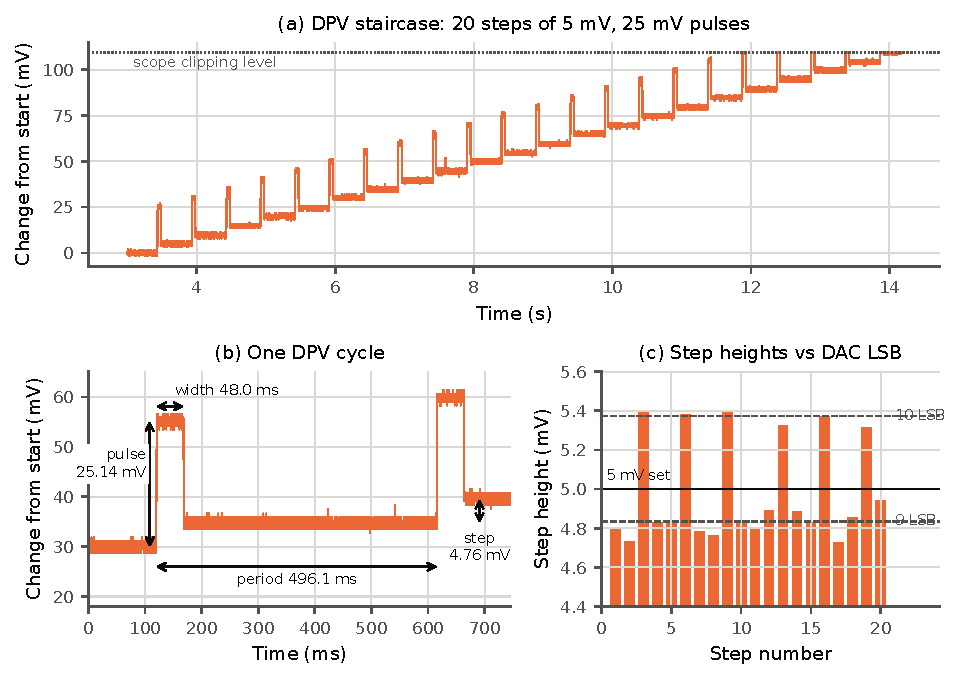
\includegraphics[width=0.78\textwidth]{figures/Testing/waveform.pdf}
\end{figure}


\subsection{Amplitude}
\label{sec:waveform_amplitude}

Every step is either \SI{4.76}{\milli\volt} or \SI{5.37}{\milli\volt} and never
deviates as illustrated in Figure~\ref{fig:waveform}c. These are 9 and
10 codes of the 12-bit DAC that sets the cell potential \cite{ad5941_ds}. A \SI{5}{\milli\volt} step is 9.31
LSB, so the firmware rounds each level to the nearest code, and the steps follow
the pattern 9, 9, 10 with a mean of \SI{4.98}{\milli\volt}. Because each level
is computed from its absolute target rather than by adding steps, the rounding
does not accumulate. The pulse is rounded to 47 LSB (\SI{25.25}{\milli\volt})
and measures \SI{25.17}{\milli\volt}. The difference between the two step
sizes, \SI{0.545}{\milli\volt}, matches the LSB to within the
\SI{\pm 3}{\percent} gain accuracy of the oscilloscope \cite{siglent_sds1000xe},
which limits how precisely the amplitudes can be verified. The applied
potential is therefore correct to within one LSB. A \SI{0.54}{\milli\volt} resolution is more than enough for DPV, where a peak is normally
about \SI{90}{\milli\volt} wide \cite{bard2001}.

\subsection{Timing}
\label{sec:waveform_timing}

The edges settle in less than \SI{0.1}{\milli\second}, which is negligible
against the \SI{50}{\milli\second} pulse. The pulse width alternates between
\SI{48.0}{\milli\second} and \SI{49.1}{\milli\second}, and the period between
two values about \SI{1}{\milli\second} apart, consistent with the
\SI{1}{\milli\second} resolution of the firmware timer. Both are shorter than
set, the pulse by \SI{1.5}{\milli\second} on average
(\SI{3}{\percent}) and the period by \SI{3.5}{\milli\second}
(\SI{0.7}{\percent}).

Timing does not affect the peak potential, which identifies the compound, so
these errors change only the peak height. For a diffusion-limited current,
which decays as $t^{-1/2}$ \cite{bard2001}, sampling \SI{3}{\percent} early
raises the measured current by about \SI{1.5}{\percent}, and the
\SI{1.1}{\milli\second} alternation varies it by about \SI{1}{\percent}
between points. The device therefore applies the programmed waveform, with
amplitudes correct to one LSB and timing within \SI{3}{\percent}. With
the excitation verified, the next check is the current it measures.

\begin{table}[H]
  \centering
  \small
  \caption{Measured excitation waveform against the programmed values.}
  \label{tab:waveform}
  \begin{tabular}{@{}l r r r@{}}
    \toprule
    \textbf{Parameter} & \textbf{Set} & \textbf{Measured} & \textbf{Error} \\
    \midrule
    Step height (20 steps)   & \SI{5}{\milli\volt}     & \SI[separate-uncertainty=true]{4.98 \pm 0.26}{\milli\volt}  & $-0.3$\,\% \\
    Pulse height (17 pulses) & \SI{25}{\milli\volt}    & \SI[separate-uncertainty=true]{25.17 \pm 0.08}{\milli\volt} & $+0.7$\,\% \\
    Pulse width              & \SI{50}{\milli\second}  & \SI[separate-uncertainty=true]{48.5 \pm 0.6}{\milli\second}  & $-3.0$\,\% \\
    Period                   & \SI{500}{\milli\second} & \SI[separate-uncertainty=true]{496.5 \pm 0.6}{\milli\second} & $-0.7$\,\% \\
    Edge time (10--90\,\%)   & --                      & $<$\SI{0.1}{\milli\second}                                 & -- \\
    \bottomrule
  \end{tabular}
\end{table}

% =====================================================================
\section{Resistor Calibration}
\label{sec:rtia_cal}

The firmware converts the high-speed TIA output to a current using the value of
the selected gain resistor $R_\text{TIA}$ \cite{ad5941_ds}, so any difference
between the nominal and the actual gain of the signal chain appears directly as
a current error. Each of the eight ranges was therefore calibrated separately.

A Plusivo DM101 digital multimeter~\cite{plusivo_dm101} was used to measure a resistor $R$, which
was connected in place of the cell. On its 2\,V DC range the multimeter has a resolution of 1\,mV
and an accuracy of $\pm0.5\,\%$, and on its 2\,k$\Omega$ to
200\,k$\Omega$ resistance ranges an accuracy of $\pm0.8\,\%$. The value of $R$ was
chosen so that $\pm0.5$\,V drives a current near the top of its operational range. At $\pm0.5$\,V
the multimeter was used to measure the voltage $V$ across the resistor, giving the true current
$I_\text{true} = V/R$, and the firmware reading $I_\text{meas}$ was recorded. Denoting the two operating points by the subscripts $+$ and $-$, a linear correction is fitted through them:
\begin{equation}
  I_\text{true} = k\,I_\text{meas} + c,
  \qquad
  k = \frac{I_{\text{true},+} - I_{\text{true},-}}{I_{\text{meas},+} - I_{\text{meas},-}},
  \qquad
  c = I_{\text{true},+} - k\,I_{\text{meas},+},
  \label{eq:rtia_cal}
\end{equation}
where the gain $k$ corrects the scale and the offset $c$ the zero. The two
points lie at opposite ends of the range, so the slope can be estimated
accurately. The correction was verified at $+\SI{0.25}{\volt}$, a point not
used in the fit.

Before calibration, $I_\text{meas}$ exceeded $I_\text{true}$ by \SIrange{9}{12}{\percent} on all
eight ranges (Table~\ref{tab:rtia_cal_tbl}). An error of the same size and sign on ranges with
different resistors points to a cause shared by the conversion chain, such as
the assumed ADC reference or PGA gain, rather than to the tolerance of the external resistors, although the internal gain resistors of the AD5941 may also share a common process error. After
correction the maximum error is \SI{0.44}{\percent}.

\begin{table}[!htbp]
  \centering
  \small
  \setlength{\aboverulesep}{0pt}
  \setlength{\belowrulesep}{0pt}
  \renewcommand{\arraystretch}{1.2}
  \caption{Two-point calibration of the high-speed TIA ranges, recomputed from
    the recorded readings. Errors are measured at $+\SI{0.25}{\volt}$.}
  \label{tab:rtia_cal_tbl}
  \begin{tabular}{@{}l r r | r | r r@{}}
    \toprule
    \textbf{Range} & \textbf{$R$ (DMM)} & \textbf{Gain $k$} & \textbf{Offset $c$ (nA)}
      & \textbf{Error before (\%)} & \textbf{Error after (\%)} \\
    \midrule
    \SI{200}{\ohm}       & \SI{994}{\ohm}         & 0.9013 & 160.0   & 11.36 & $+0.44$ \\
    \SI{1}{\kilo\ohm}    & \SI{994}{\ohm}         & 0.9141 & 278.7   &  9.70 & $+0.40$ \\
    \SI{5}{\kilo\ohm}    & \SI{4.59}{\kilo\ohm}   & 0.9089 & $-69.5$ &  9.99 & $-0.16$ \\
    \SI{10}{\kilo\ohm}   & \SI{9.93}{\kilo\ohm}   & 0.8971 & $-81.6$ & 11.78 & $-0.05$ \\
    \SI{20}{\kilo\ohm}   & \SI{19.9}{\kilo\ohm}   & 0.9018 & $-15.8$ & 11.09 & $+0.06$ \\
    \SI{40}{\kilo\ohm}   & \SI{38.5}{\kilo\ohm}   & 0.9129 & $-9.2$  &  9.72 & $+0.02$ \\
    \SI{80}{\kilo\ohm}   & \SI{81.5}{\kilo\ohm}   & 0.9158 & $-3.0$  &  9.44 & $+0.13$ \\
    \SI{160}{\kilo\ohm}  & \SI{146.7}{\kilo\ohm}  & 0.9191 & $1.1$   &  9.15 & $+0.38$ \\
    \bottomrule
  \end{tabular}
\end{table}

With the gain of every range corrected and checked against an independent
reference, the current scale of the device is known to within about
$\pm$\SI{1}{\percent}, limited by the multimeter used as the reference. This is crucial from an application perspective because the drug concentration is calculated
directly from the peak current. The next test uses Randles circuits and adds a capacitive load to the system.

% =====================================================================
\section{Randles Circuit Test}
\label{sec:randles_test}

The next test adds the capacitance of the cell. A real electrode has a
double-layer capacitance, which the DPV sampling of Section~\ref{sec:dpv_rejection} is designed
to reject. The Randles test checks this with passive networks of known DC
resistance in place of the cell \cite{c5}. A total of 7 test cells were used, three cells of the PalmSens4 dummy cell (WE~A to~C) and four networks built for this project (Cells~1 to~4), each scanned on both instruments. Once the capacitors have charged, the
DPV current depends only on the DC path, so the expected value is
$\Delta I = \Delta E_\text{pulse}/(R_s + R_{ct})$ with
$\Delta E_\text{pulse} = \SI{25}{\milli\volt}$, and zero for the networks with a
series capacitor (WE~A and Cell~2). The mean $\Delta I$ over the scan was
compared with this value, and the noise was taken as the standard deviation
(Table~\ref{tab:randles}).

\begin{table}[!htbp]
  \centering
  \footnotesize
  \setlength{\tabcolsep}{3pt}
  \caption{Ferricyanide DPV scans. Measured on its own drop, \SIrange{0.8}{1.3}{\volt}}
  \label{tab:randles}
  \begin{tabular}{@{}l l r r r r r r@{}}
    \toprule
    & & \textbf{Expected} & \multicolumn{2}{c}{\textbf{Mean $\Delta I$ (nA)}}
      & \multicolumn{2}{c}{\textbf{Error (\%)}} & \textbf{Noise (nA)} \\
    \cmidrule(lr){4-5}\cmidrule(lr){6-7}
    \textbf{Cell} & \textbf{Network} & \textbf{(nA)} & \textbf{PS4} & \textbf{\devname}
      & \textbf{PS4} & \textbf{\devname} & \textbf{PS4 / \devname} \\
    \midrule
    WE A   & $560\,\Omega + (33\,\text{nF} \parallel \text{diodes})$ & 0      & 0.00   & 0.01   & --      & --      & 0.10 / 0.07 \\
    WE B   & $10\,\text{k}\Omega$                                     & 2500.0 & 2504.4 & 2511.0 & $+0.18$ & $+0.44$ & 6.0 / 8.2 \\
    WE C   & $560\,\Omega + (33\,\text{nF} \parallel 10\,\text{k}\Omega)$ & 2367.4 & 2372.0 & 2380.5 & $+0.19$ & $+0.55$ & 5.4 / 6.1 \\
    Cell 1 & $93.8\,\text{k}\Omega$                                   & 266.5  & 264.9  & 269.7  & $-0.62$ & $+1.19$ & 2.2 / 0.8 \\
    Cell 2 & $9.83\,\text{k}\Omega + 470\,\text{nF}$                  & 0.05   & 0.11   & 0.21   & --      & --      & 0.38 / 0.09 \\
    Cell 3 & $556\,\Omega + (97.5\,\text{k}\Omega \parallel 1\,\mu\text{F})$ & 255.0 & 254.9 & 259.7 & $-0.02$ & $+1.88$ & 1.0 / 1.4 \\
    Cell 4 & $556\,\Omega + (923\,\text{k}\Omega \parallel 1\,\mu\text{F})$  & 32.4  & 33.1  & 32.4  & $+2.04$ & $-0.08$ & 0.7 / 1.2 \\
    \bottomrule
  \end{tabular}
\end{table}


Both instruments measured every network with a DC path to within
\SI{2.1}{\percent} of the expected value. The \devname{} read slightly high on
all of them except Cell~4, by \SIrange{0.4}{0.6}{\percent} on the
\SI{2.5}{\micro\ampere} networks and \SIrange{1.2}{1.9}{\percent} on the
\SI{260}{\nano\ampere} networks. The
blocking networks WE~A and Cell~2 read below \SI{0.25}{\nano\ampere} on both
instruments, so the charging current is rejected and there is no DC leakage
path. The noise on these two networks, \SIrange{0.07}{0.09}{\nano\ampere}, is the floor of the instrument itself; with the estimate of Section~\ref{sec:dpv_applications}, its $3\sigma$ of about \SI{0.25}{\nano\ampere} corresponds to roughly \SIrange{1}{5}{\micro\gram\per\litre} of efavirenz.

\begin{figure}[H]
  \caption{DPV scans of the dummy cell WE~C (Left) and Cell~3 (Right) from \SIrange{0.8}{1.3}{\volt}.}
  \label{fig:randles_curves}
  \centering
  \begin{minipage}[t]{0.49\textwidth}
    \centering
    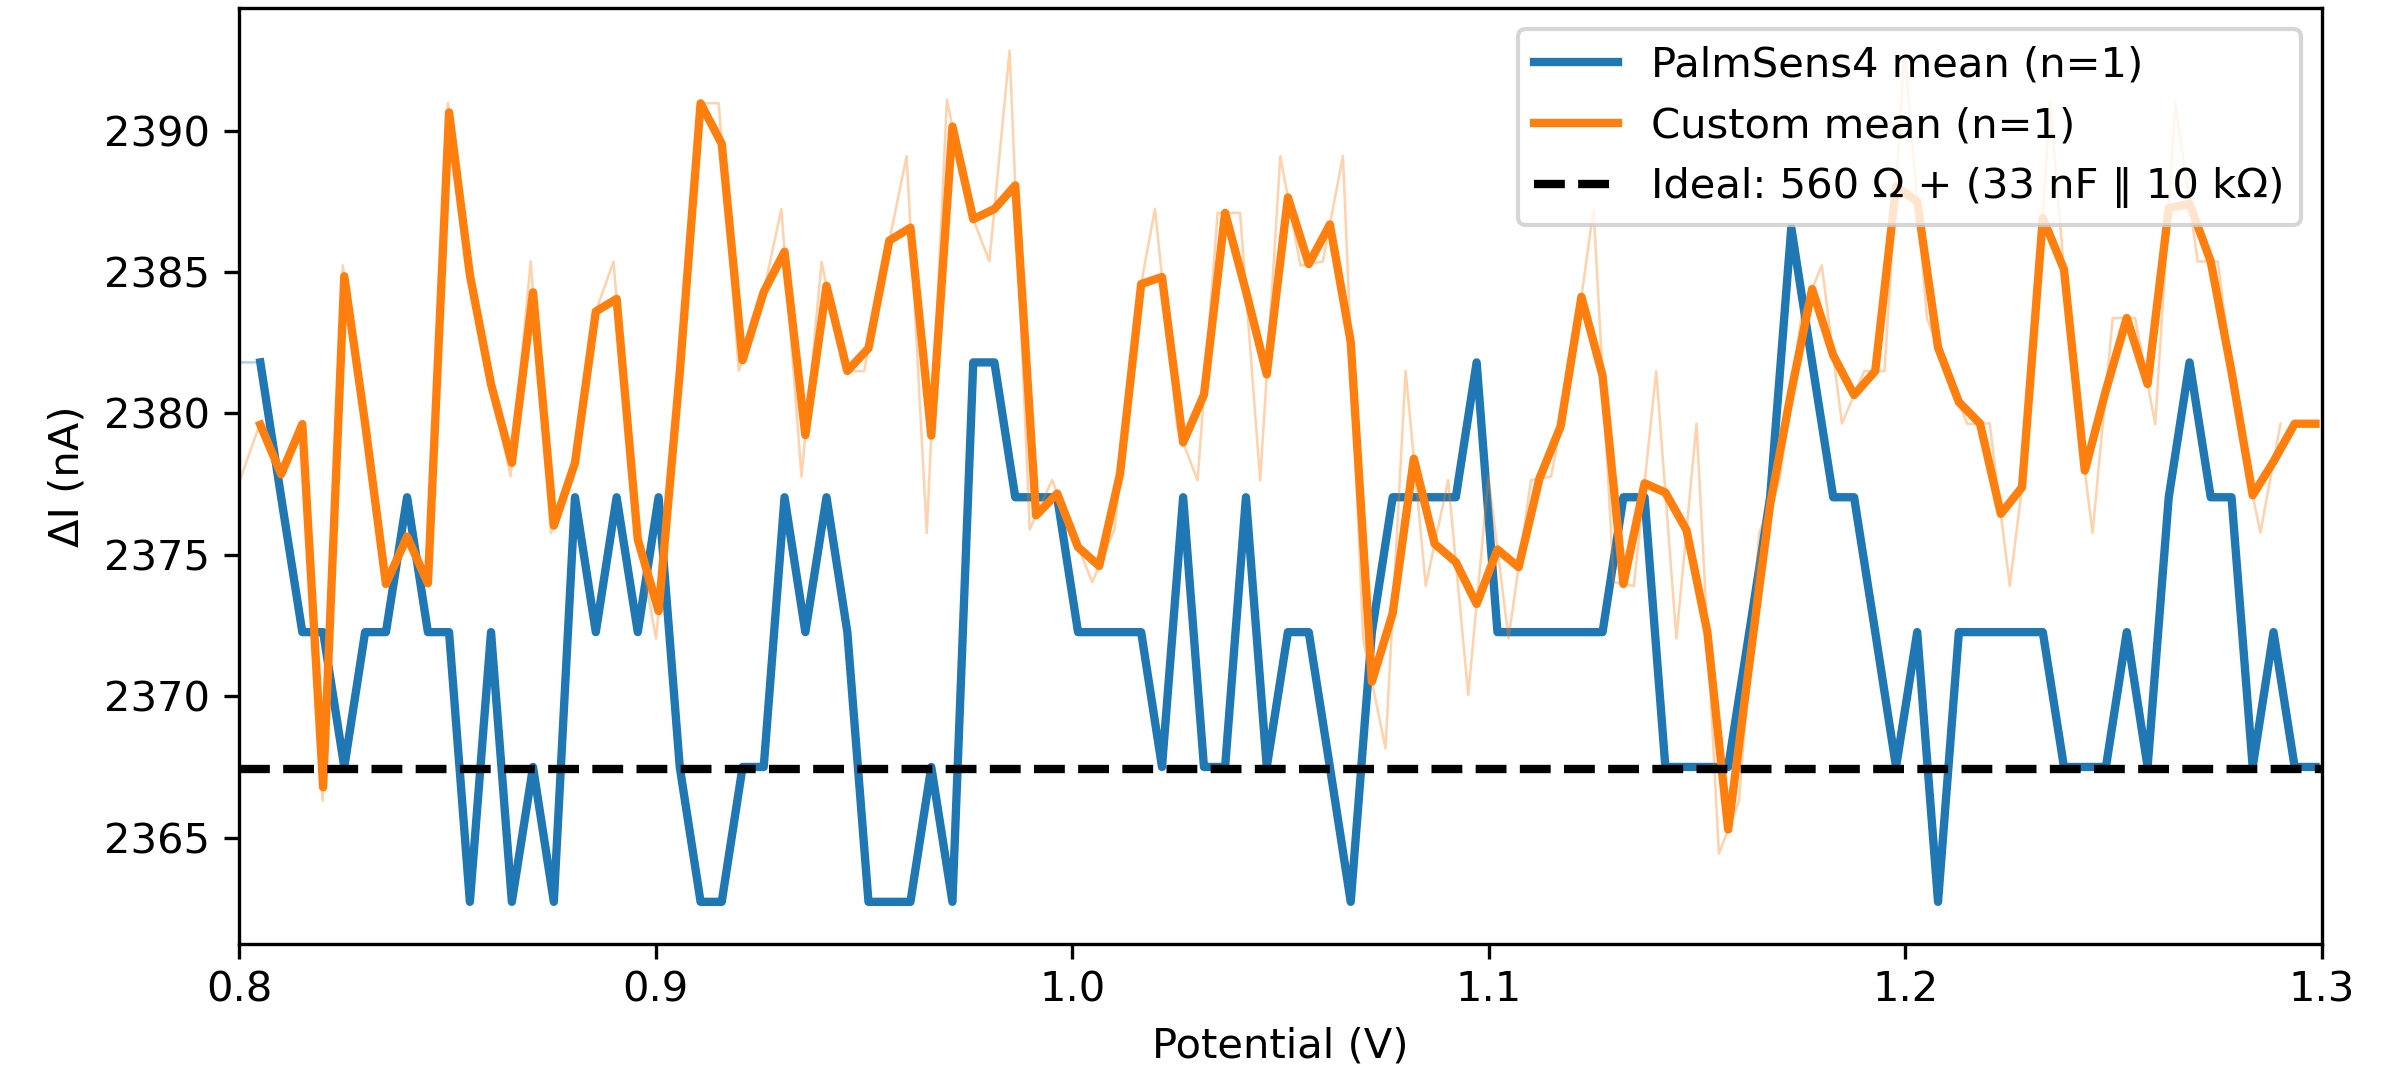
\includegraphics[width=\textwidth]{figures/Testing/randles_wec_top.png}
  \end{minipage}\hfill
  \begin{minipage}[t]{0.49\textwidth}
    \centering
    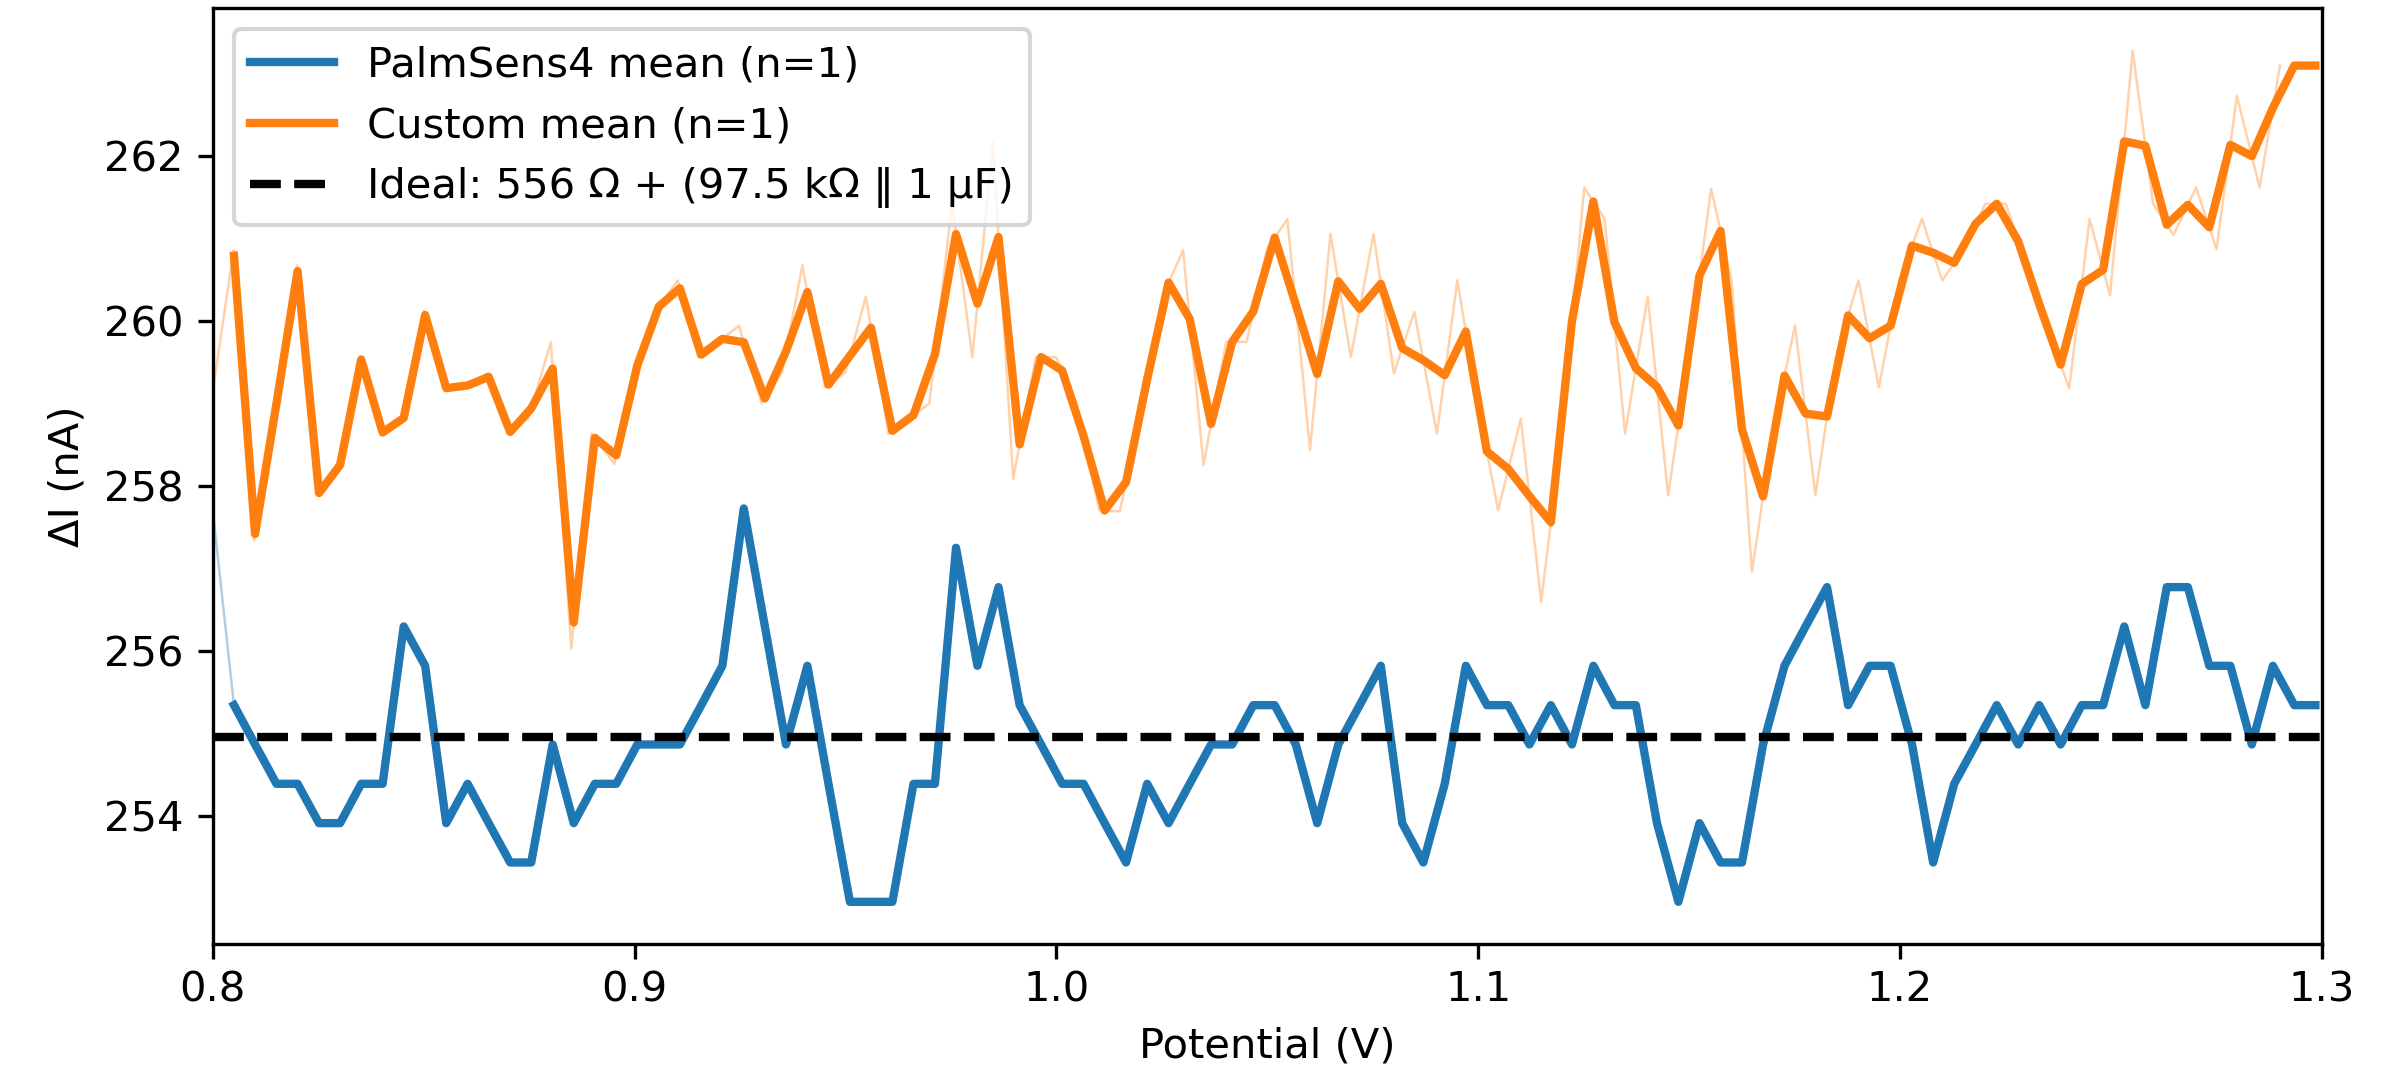
\includegraphics[width=\textwidth]{figures/Testing/randles_cell3_top.png}
  \end{minipage}
\end{figure}

The next two tests replace the known load with a real electrode. From this
point the true value is no longer known, so the PalmSens4 becomes the
reference, and its own scan-to-scan variation becomes a variable.

% =====================================================================
\section{Salt Solution Test}
\label{sec:salt_test}

The fourth test replaces the passive circuit with a real electrode. A drop of
\SI{0.1}{\Molar} KCl on the SPE has a solution resistance and a
double-layer capacitance, but no redox reaction in the scan window, which makes
it a physical Randles cell with a very large charge-transfer resistance
\cite{bard2001}. Figure~\ref{fig:pair}b shows the setup used for the salt blank tests. It should give a smooth background without a peak. The
\devname{} is judged against the PalmSens4 measuring the same solution with the
same waveform parameters.

Five pairs of salt were compared, Salt~1 to~5 as seen in Figure~\ref{fig:salt_pairs}, each consisting of one scan on each instrument on the same drop. Table~\ref{tab:salt} compares each pair quantitatively, using the mean current, the RMS difference and the correlation between the two voltammograms. The comparison runs from \SI{0.40}{\volt} to \SI{-0.20}{\volt}, so that the ferricyanide peak of Section~\ref{sec:fc_test} lies in the window.

\begin{figure}[H]
\caption{Salt solution measured by each potentiostat.}
  \label{fig:salt_pairs}
  \centering
  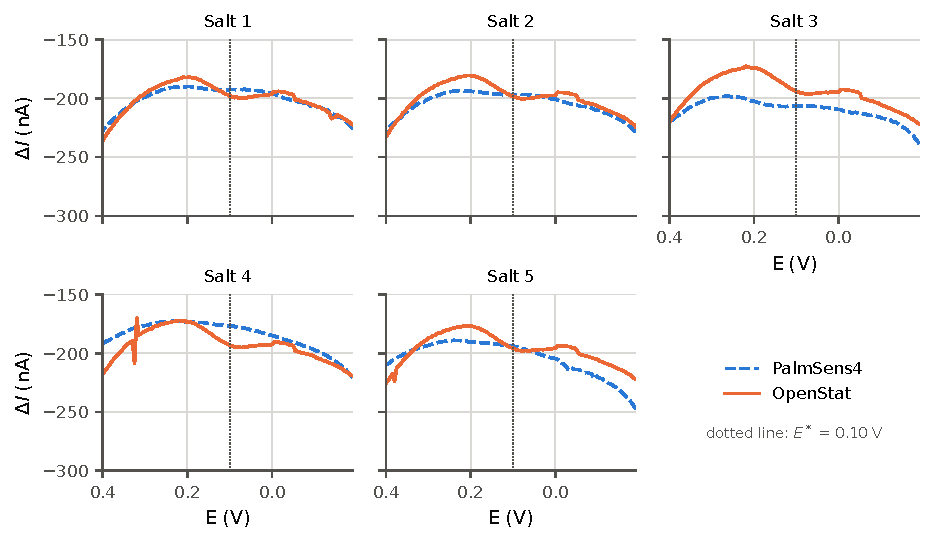
\includegraphics[width=0.7\textwidth]{figures/Testing/salt_pairs}
\end{figure}

\begin{table}[H]
  \centering
  \small
\caption{Salt test. All scans on the OpenStat used the
  $\SI{80}{\kilo\ohm}$ range. $r$ is the correlation coefficient between the PS4 and
  OpenStat voltammograms of each pair.}
    \label{tab:salt}
  \begin{tabular}{@{}l r r r r r r@{}}
    \toprule
    & \multicolumn{2}{c}{\textbf{Mean $\Delta I$ (nA)}} & \textbf{Dev.}
      & \textbf{RMS} & \textbf{Noise (nA)} & \\
    \cmidrule(lr){2-3}
    \textbf{Pair} & \textbf{PS4} & \textbf{\devname}
      & \textbf{(\%)} & \textbf{(nA)} & \textbf{PS4 / \devname} & \textbf{$r$} \\
    \midrule
    Salt 1 & $-200.7$ & $-200.0$ & $-0.3$ & 4.5  & 0.6 / 0.9 & 0.94 \\
    Salt 2 & $-204.0$ & $-199.3$ & $-2.3$ & 6.6  & 0.6 / 0.8 & 0.93 \\
    Salt 3 & $-209.6$ & $-194.0$ & $-7.4$ & 16.8 & 0.6 / 0.8 & 0.90 \\
    Salt 4 & $-184.7$ & $-192.4$ & $+4.1$ & 10.2 & 0.5 / 3.1 & 0.86 \\
    Salt 5 & $-204.2$ & $-196.4$ & $-3.8$ & 11.7 & 0.7 / 1.1 & 0.80 \\
    \bottomrule
  \end{tabular}

\end{table}


With no analyte present the current measured varies from \SIrange{-185}{-210}{\nano\ampere} on the PalmSens4 and
\SIrange{-192}{-200}{\nano\ampere} on the \devname{} as shown in Figure~\ref{fig:salt_pairs} and 
Table~\ref{tab:salt}. The mean deviation per measured pair ranges from
\SI{-7.4}{\percent} to \SI{+4.1}{\percent} and the RMS difference from
\SIrange{4.5}{16.8}{\nano\ampere}. This is larger than in the Randles test, but is of similar size as the variation of the cell itself. This is shown from scan to scan where
the PalmSens4 measurement has a standard deviation of
\SI{10.4}{\nano\ampere}, and the \devname{} \SI{3.5}{\nano\ampere}.

\section{Ferricyanide Test}
\label{sec:fc_test}
 
The last test adds a redox reaction. Ferricyanide gives a single,
well-understood reduction peak, so it tests the potential axis and the current scale together \cite{bard2001}.
\begin{equation}
  [\text{Fe(CN)}_6]^{3-} + e^- \rightleftharpoons [\text{Fe(CN)}_6]^{4-},
\end{equation}
All \devname{} scans used the \SI{1}{\kilo\ohm} range. Three
pairs were compared, FC~1 to~3, each consisting of one scan on each instrument
on a different drop as seen in Figure~\ref{fig:fc_pairs}.
 
\begin{figure}[!htbp]
  \caption{Ferricyanide DPV scans on the same drop, \devname{} run against PalmSens4 run.}
  \label{fig:fc_pairs}
  \centering
  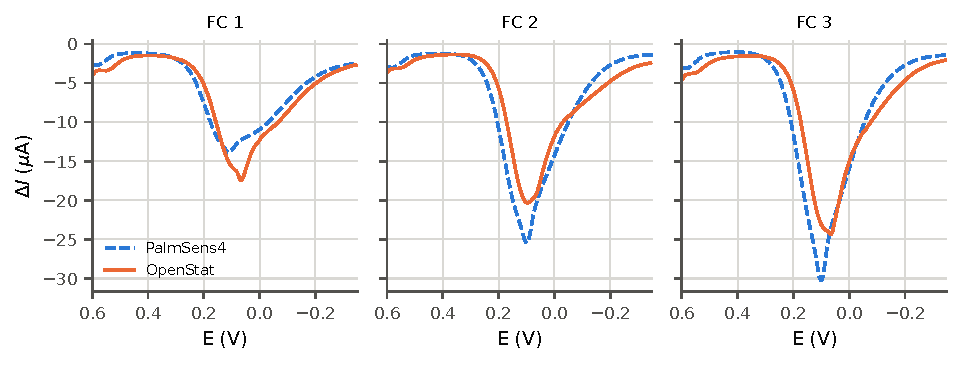
\includegraphics[width=0.8\textwidth]{figures/Testing/fc_pairs.pdf}
\end{figure}
 
The \devname{} produces a peak similar in shape to the PalmSens4 shown in its correlation $r \geq 0.956$ for
all three pairs. However, there are two visible differences: the peak heights differ by up to $\pm$\SI{26}{\percent} and the \devname{} peak lies
at a more negative potential (shifted to the right).
 
\subsection{Peak Height}
\label{sec:fc_height}
 
The peak heights of the three pairs are plotted in
Figure~\ref{fig:pair}a.
 

\begin{figure}[htbp]
  \centering
  \caption{The three ferricyanide pairs. (a) Peak height of the \devname{}
    against the PalmSens4. (b) \devname{} testing setup, either solution applied to the SPE by mechanical pipette.}
  \label{fig:pair}
  \begin{minipage}[b]{0.38\textwidth}
    \centering
    \includegraphics[width=\linewidth]{figures/testing/fc_compare_a.png}\\
    (a)
  \end{minipage}
  \hfill
  \begin{minipage}[b]{0.48\textwidth}
    \centering
    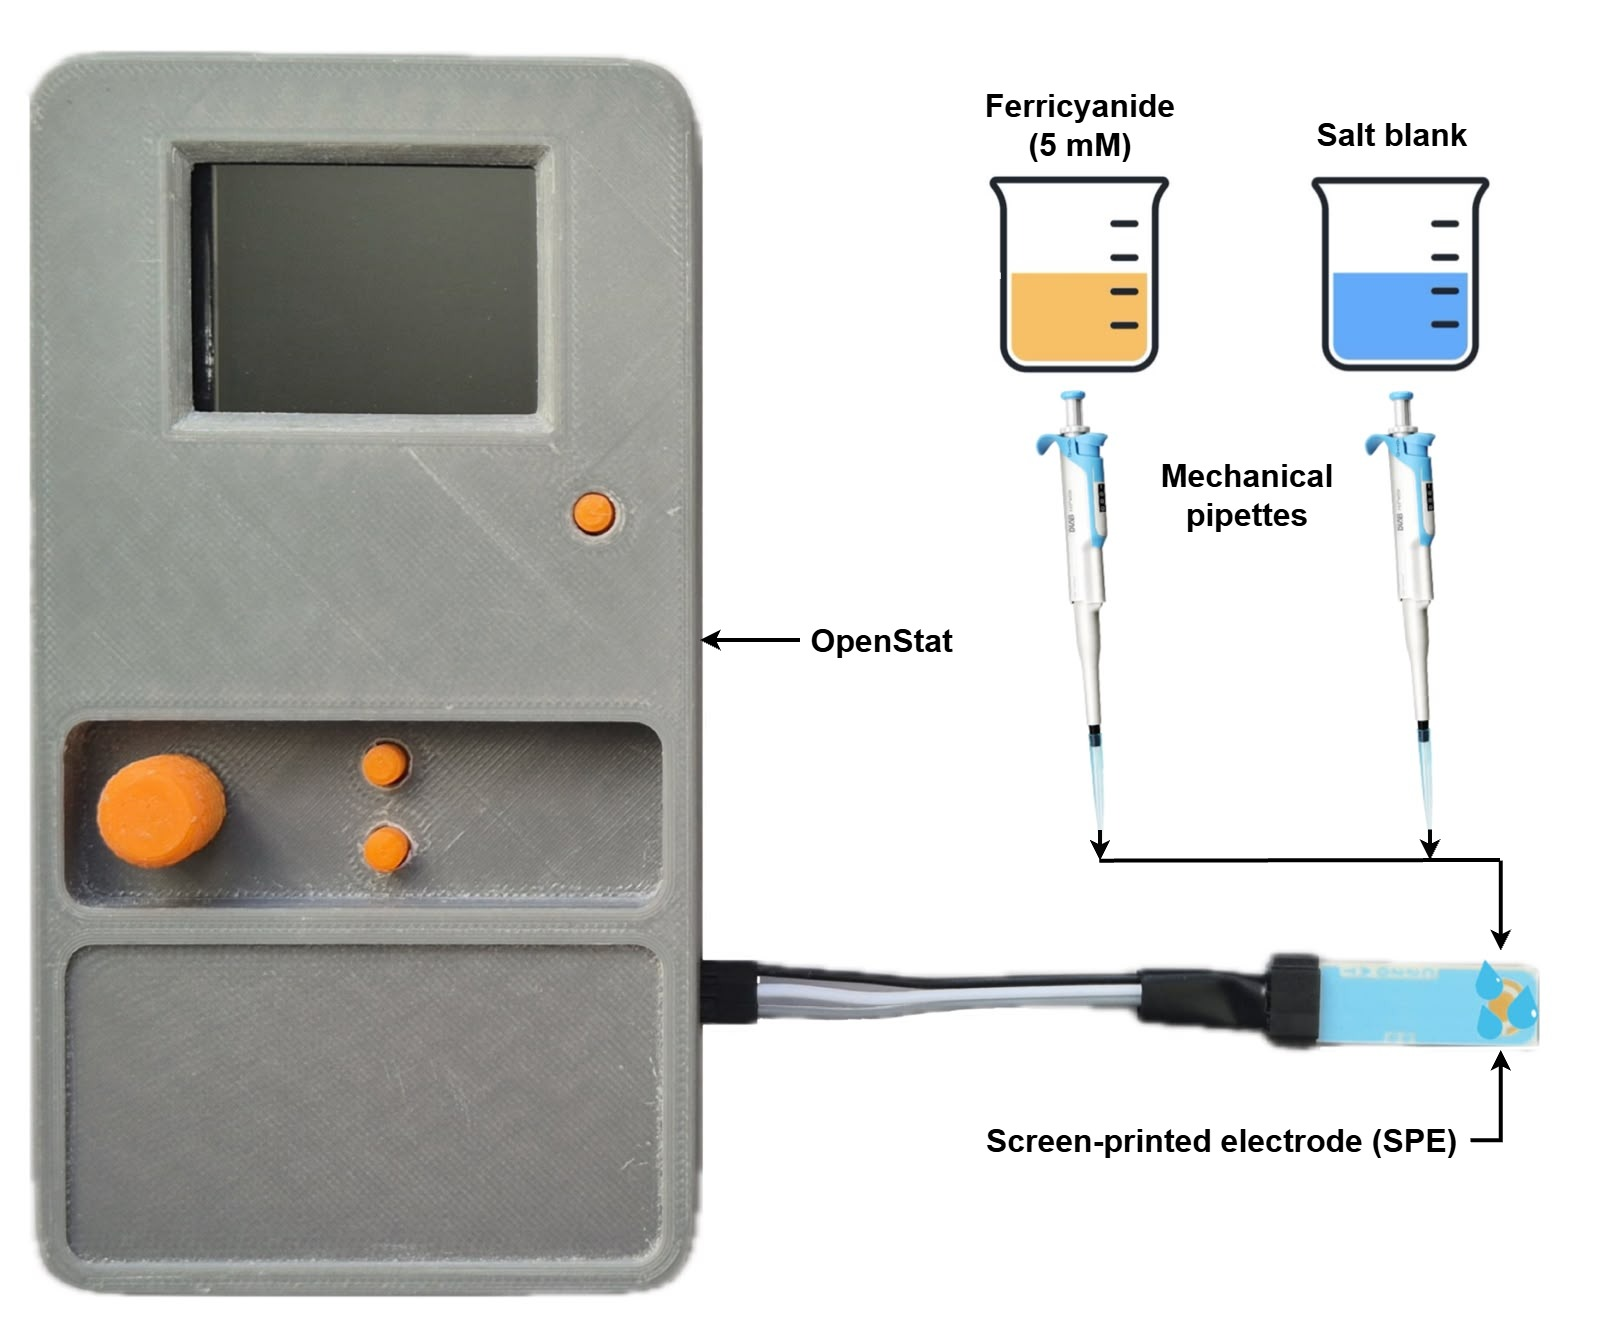
\includegraphics[width=\linewidth]{figures/testing_steps.jpg}\\
    (b)
  \end{minipage}
\end{figure}

 
The \devname{} overestimates peak height by \SI{26}{\percent} on FC~1 and underestimates it by approximately \SI{20}{\percent} on FC~2 and~3, indicating bidirectional deviation rather than regular bias. This difference must be judged against the repeatability of each instrument. Consecutive PalmSens4 scans were taken to verify this, and they vary by \SIrange{8}{52}{\percent}, while consecutive \devname{} scans vary by \SIrange{3}{33}{\percent}. The mean difference between the instruments, \SI{22}{\percent}, falls within the repeatability of the reference itself, so the test shows no instrument difference larger than the variation of the electrode, but cannot detect a smaller one. Because evaporation raises the peak over time, the later scans are expected to read higher.
 
\subsection{Peak Potential}
\label{sec:fc_shift}
 
The potential offset was found by sliding the \devname{} curve of each pair
along the potential axis until it matched the
PalmSens4 curve most closely. The offset ranges from \SIrange{20}{27.5}{\milli\volt}, where \SI{24}{\milli\volt} is the average. Shifting the \devname{} curve reduces the difference between the curves by up to a third. All the \devname{} ferricyanide scans used the \SI{1}{\kilo\ohm} range, therefore the offset
could potentially come from the specific range or its calibration. The calibration
cannot cause it, as it only rescales the current. A range-dependent cause would act through a voltage drop proportional to the
current, so the offset would grow with the peak; instead, it stays the same
while the peak more than doubles from FC~1 to FC~3
(Figure~\ref{fig:fc_pairs}). The \devname{} records each point at its base potential (Section~\ref{sec:sw_scan_flow}), and the offset is close to half of the \SI{50}{\milli\volt} pulse, which suggests that the instruments report the potential of a point at different positions within the step. Repeating a scan with a \SI{25}{\milli\volt} pulse would test this, as the offset should then halve. Until the cause is confirmed, the offset must be corrected before peak potentials are compared with published values.
 
 
\subsection{Sources of Deviation}
\label{sec:fc_deviation}
 
The remaining differences come from the solution and the testing environment, which drift between scans. Because the two instruments never measure the same drop at the same moment, this drift enters every comparison. Likely causes are:
\begin{itemize}[label=\textbullet]
  \item \textbf{Adsorption.} Gold is not inert in ferricyanide; when cyanide is 
    released from the complex and adsorbs on the gold, the gold is slowly etched. This results in the active area and electron-transfer rate to change from scan to scan \cite{vogt2016,lazar2016}. This could explain the low and varying peak currents and the movement of the peak potential.
  \item \textbf{Light sensitivity.} Ferricyanide decomposes when exposed to light; it breaks down into ferrocyanide and releases cyanide \cite{murton2025}. During every scan the drop on the electrode is exposed to room light, which lowers its ferricyanide concentration and adds cyanide that attacks the gold.
  \item \textbf{Evaporation.} A small drop loses water within minutes, which
    raises its concentration and explains why repeat scans on one drop grow in peak height rather than shrink.
\end{itemize}
The comparison would improve by using a fresh electrode for each pair,
shielding the drop from light, and starting each scan at a fixed time after the
drop is placed. 
 
\section{Summary}
\label{sec:testing_summary}
 
Table~\ref{tab:testing_summary} checks each objective of Section~\ref{sec:project_aim_obj_scope} against its target.

\begin{table}[!htbp]
  \caption{Verification of the project objectives.}
  \label{tab:testing_summary}
  \centering
  \footnotesize
  \begin{tabularx}{\textwidth}{@{}>{\raggedright\arraybackslash}p{2.0cm} >{\raggedright\arraybackslash}p{3.6cm} >{\raggedright\arraybackslash}X l@{}}
    \toprule
    \textbf{Objective} & \textbf{Target} & \textbf{Result} & \textbf{Status} \\
    \midrule
    1 Waveform   & LSB $\leq$ \SI{1}{\milli\volt}; pulse \SI{25}{\milli\volt} $\pm$ \SI{1}{\milli\volt}; period $\pm$\SI{1}{\percent}
                 & LSB \SI{0.54}{\milli\volt}; pulse \SI{25.17}{\milli\volt}; period \SI{-0.7}{\percent}; width \SI{-3}{\percent} (about \SI{1.5}{\percent} in current) & Met \\
    2 Current    & $\pm$\SI{750}{\micro\ampere}; sub-nA resolution; gain error $\leq$ \SI{1}{\percent}
                 & \SI{0.23}{\nano\ampere} per code; $\leq$ \SI{0.44}{\percent} after calibration (reference $\pm$\SI{1}{\percent}); overload at \SI{720}{\micro\ampere} in normal & Partly met \\
    3 Agreement  & Dummy cells; PalmSens4 within its repeatability
                 & Dummy cells within \SI{1.9}{\percent}; salt and ferricyanide within PalmSens4 repeatability; \SI{24}{\milli\volt} offset & Partly met \\
    4 Interfaces & Standalone and web browser operation
                 & Both demonstrated (Figure~\ref{fig:interface}, Section~\ref{sec:sw_scan_flow}) & Met \\
    5 Battery    & At least \SI{8}{\hour}
                 & \SIrange{18}{24}{\hour}, estimated from measured current (Section~\ref{sec:hw_battery}) & Met (estimate) \\
    6 Cost       & Report and compare
                 & R2\,226 incl.\ VAT (Appendix~\ref{app:bom}), against approximately R55\,400 for the PalmSens4 & Met \\
    \bottomrule
  \end{tabularx}
\end{table}

The bench tests confirm the electronics. The electrochemical comparisons were limited by the repeatability of the electrode rather than the instrument, and the \SI{24}{\milli\volt} offset remains to be explained.

\graphicspath{{conclusion/fig/}}

\chapter{Conclusion and Future Work}
\label{chap:conclusion}

\providecommand{\devname}{OpenStat}
\section{Conclusion}
\label{sec:conclusion}

This project set out to design, build and validate a low-cost, wireless potentiostat for the DPV detection of efavirenz and oseltamivir in water. Against the objectives of Section~\ref{sec:project_aim_obj_scope} (Table~\ref{tab:testing_summary}), the \devname{} applies the DPV waveform to within one DAC code (Objective~1); reads every current range to within \SI{0.44}{\percent} after calibration but overloads above \SI{720}{\micro\ampere} instead of \SI{750}{\micro\ampere} when in normal mode (Objective~2, partly met). The OpenStat agreed with dummy cells to within \SI{1.9}{\percent} and with the PalmSens4 within that instrument's own repeatability, apart from a \SI{24}{\milli\volt} offset (Objective~3, partly met). The device can be controlled physically or from a web browser (Objective~4) for an estimated \SIrange{18}{24}{\hour} per charge (Objective~5). It costs R2\,226, against US\$3\,340 for the PalmSens4 (Objective~6). The electrochemical tests were limited by the repeatability of the electrode, and the target drugs were not measured, so the detection limit was not measured; the noise floor suggests roughly \SIrange{1}{5}{\micro\gram\per\litre} for the electronics alone (Section~\ref{sec:randles_test}).

\section{Future Work}
\label{sec:future_work}

The \SI{24}{\milli\volt} offset should be investigated first, by repeating a ferricyanide scan with a \SI{25}{\milli\volt} pulse (Section~\ref{sec:fc_shift}) and on other current ranges. A ferricyanide concentration series on both instruments would then give the sensitivity and detection limit, and the noise floor should be measured with Wi-Fi on and off. In the firmware, starting each averaging window \SI{20}{\milli\second} before its edge would reduce the timing error (Section~\ref{sec:sw_limitations}), raising $C_f$ to \SI{63}{\pico\farad} would improve the phase margin with small-capacitance electrodes (Section~\ref{sec:stability}), and peak detection would let the device report peak height and potential. The hardware needs a grounded, shielded electrode cable (Section~\ref{sec:hw_ground}), the high-power mode of the potentiostat amplifier for the \SI{200}{\ohm} range (Section~\ref{sec:sw_ranges}), and a charger with power-path control so that it can run while charging. The device should then be tested with efavirenz and oseltamivir, using preconcentration or a modified electrode; machine learning could then be used to identify and quantify compounds whose peaks overlap.


% Bibliography
\chapter*{References}\markboth{}{\scshape References}
\addcontentsline{toc}{chapter}{References}
\renewcommand{\bibsection}{}
\bibliography{mybib}

% End matter
\appendix
\chapter{AD5941 Capacitor Selection}{}
\makeatletter\@mkboth{}{Appendix}\makeatother
\label{appen:hw_caps}

Table~\ref{tab:hw_caps} lists the capacitors around the AD5941 and the
justification for each value, as discussed in Section~\ref{sec:hw_caps}.

\begin{table}[H]
  \centering
  \caption{Capacitors around the AD5941 and the justification for each value.}
  \label{tab:hw_caps}
  \footnotesize
  \setstretch{1}
  \renewcommand{\arraystretch}{1.3}
  \setlength{\tabcolsep}{4pt}
  \begin{tabularx}{\textwidth}{@{}l l l
      >{\raggedright\arraybackslash}p{3.7cm}
      >{\raggedright\arraybackslash}X@{}}
    \toprule
    \textbf{Ref} & \textbf{Pin} & \textbf{Value} & \textbf{Role} & \textbf{Reason} \\
    \midrule
    C7, C24 & DVDD (6)   & \SI{100}{\nano\farad} & HF supply decoupling
        & Two-tier convention \cite{adi_mt101}; target impedance \cite{smith1999pds} \\
    C30 & IOVDD (26)     & \SI{100}{\nano\farad} & HF decoupling of SPI drivers
        & Two-tier convention \cite{adi_mt101}; one capacitor per pin \\
    C31 & AVDD (30)      & \SI{100}{\nano\farad} & HF supply decoupling
        & Two-tier convention \cite{adi_mt101}; local to pin 30 \\
    C33 & AVDD (41)      & \SI{100}{\nano\farad} & HF supply decoupling
        & Two-tier convention \cite{adi_mt101}; local to pin 41 \\
    C9  & AVDD (30)      & \SI{10}{\micro\farad} & Bulk decoupling; LC filter with FB1
        & Meets \SI{1}{\ohm} target above \SI{16}{\kilo\hertz} \cite{smith1999pds} \\
    C1  & \texttt{AVDD\_REG} (5) & \SI{470}{\nano\farad} & Internal LDO output capacitor
        & No datasheet value; matched to \texttt{DVDD\_REG\_1V8}
          \cite[p.~21]{ad5941_ds}, \cite{rinconmora2009ldo} \\
    C8  & \texttt{DVDD\_REG\_1V8} (14) & \SI{470}{\nano\farad} & Internal LDO output capacitor
        & Datasheet value \cite[p.~21]{ad5941_ds} \\
    C6  & \texttt{VREF\_2V5} (4) & \SI{470}{\nano\farad} & \SI{2.5}{\volt} reference decoupling
        & Datasheet value and test condition \cite[pp.~11, 20]{ad5941_ds} \\
    C10 & \texttt{VREF\_1V82} (43) & \SI{4.7}{\micro\farad} & ADC \SI{1.82}{\volt} reference reservoir
        & Datasheet recommendation \cite[p.~19]{ad5941_ds}; kickback bound \\
    C5  & \texttt{VBIAS\_CAP} (31) & \SI{470}{\nano\farad} & ADC \SI{1.11}{\volt} common-mode decoupling
        & Datasheet value and test condition \cite[pp.~11, 20]{ad5941_ds} \\
    C27 & \texttt{VBIAS0} (8) & \SI{100}{\nano\farad} & LP DAC output noise filter
        & Datasheet value \cite[p.~20]{ad5941_ds} \\
    C28 & \texttt{VZERO0} (9) & \SI{100}{\nano\farad} & LP DAC output noise filter
        & Datasheet value \cite[p.~20]{ad5941_ds} \\
    C29 & \texttt{RESET} (22) & \SI{100}{\nano\farad} & Reset hold and deglitch ($R_8 = \SI{10}{\kilo\ohm}$)
        & $\tau = \SI{1}{\milli\second} \gg \SI{1}{\micro\second}$ minimum pulse \cite[p.~14]{ad5941_ds} \\
    \bottomrule
  \end{tabularx}
\end{table}


% =====================================================================
%  Appendix -- Derivations for Chapter 3
%
%  Add to the report after \appendix with:   \input{appendix_modeling}
%  Labels referenced from system_modeling.tex:
%     app:dpv, app:feedback, app:beta, app:tia
%  Citation keys are the same as in system_modeling.tex (see its header).
% =====================================================================

\chapter{Derivations for the System Model}
\label{app:modeling}

This appendix gives the derivations behind the results used in
Chapter~\ref{chap:modeling}.

% ---------------------------------------------------------------------
\section{Capacitive Current Rejection in DPV}
\label{app:dpv}

After a potential step, the total current at the electrode is the sum of the
faradaic and capacitive components,
\begin{equation}
  I_\text{total}(t) = I_f(t) + I_c(t),
\end{equation}
with $I_c$ and $I_f$ given by Equations~\eqref{eq:ic}
and~\eqref{eq:cottrell}. Expanding the two DPV samples into these components
gives
\begin{equation}
  \Delta I = I_\text{end} - I_\text{before}
    = \left(I_{f,\text{end}} + I_{c,\text{end}}\right)
    - \left(I_{f,\text{before}} + I_{c,\text{before}}\right).
  \label{eq:app_delta_i_expanded}
\end{equation}
$I_\text{before}$ is sampled after the electrode has been held at the
baseline potential for long enough that the previous capacitive transient
has decayed, so $I_{c,\text{before}} \approx 0$. $I_\text{end}$ is sampled at
the end of a pulse that is long compared with $R_sC_{dl}$, so the transient
caused by the pulse has also decayed and $I_{c,\text{end}} \approx 0$.
Equation~\eqref{eq:app_delta_i_expanded} therefore reduces to
Equation~\eqref{eq:delta_if}, leaving only the faradaic signal.

Because $\Delta I$ is the change in faradaic current caused by a small
potential change $\Delta E$, it approximates the derivative of the
current--potential curve:
\begin{equation}
  \Delta I \approx \frac{\mathrm{d}I_f}{\mathrm{d}E}\,\Delta E.
\end{equation}
For a reversible system governed by the Nernst equation, the current--potential
curve is sigmoidal, and its derivative is a peak centred close to the
half-wave potential $E_{1/2}$, offset from it by half the pulse amplitude
\cite{bard2001, Laborda2014}.

% ---------------------------------------------------------------------
\section{Negative-Feedback Stability}
\label{app:feedback}

Both the control loop and the TIA loop have the structure of
Figure~\ref{fig:app_feedback}, where $A(s)$ is the amplifier and $\beta(s)$
is the feedback network.

\begin{figure}[htbp]
  \centering
  % KEEP: your existing control loop block diagram (old Figure 3.3).
  \caption{Control loop block diagram for the analog front-end.}
  \label{fig:app_feedback}
\end{figure}

The closed-loop transfer function is \cite{c2}
\begin{equation}
  T(s) \equiv \frac{e_o(s)}{E_\text{in}(s)} = \frac{A(s)}{1 + A(s)\beta(s)},
  \label{eq:app_closed_loop}
\end{equation}
and the loop gain is
\begin{equation}
  L(s) \equiv A(s)\beta(s).
\end{equation}
The poles of $T(s)$, which govern the transient response, are the roots of
the characteristic equation $1 + L(s) = 0$. At the crossover frequency
$\omega_c$, where $|L(j\omega_c)| = 1$, the phase margin is
\begin{equation}
  \phi_\text{PM} = \SI{180}{\degree} + \angle L(j\omega_c).
\end{equation}
If $\phi_\text{PM} \le \SI{0}{\degree}$, the closed-loop poles lie in the
right half of the $s$-plane and the system oscillates \cite{c2}.

% ---------------------------------------------------------------------
\section{Control-Loop Feedback Factor}
\label{app:beta}

In the reduced cell of Figure~\ref{fig:cell_buffer}, $R_u$ and $C_{dl}$ form
a series path from the control amplifier output $e_o(s)$ to the virtual
ground at the WE. The current through this path is
\begin{equation}
  I(s) = \frac{e_o(s)}{R_u + \dfrac{1}{sC_{dl}}},
\end{equation}
and the RE senses the voltage across the capacitive branch,
\begin{equation}
  E_\text{ref}(s) = I(s) \cdot \frac{1}{sC_{dl}}.
\end{equation}
Combining the two gives the feedback factor of Equation~\eqref{eq:beta}:
\begin{equation}
  \beta(s) \equiv \frac{E_\text{ref}(s)}{e_o(s)}
    = \frac{1}{1 + sR_uC_{dl}}.
\end{equation}
This single-pole cell model is the one used in the classical potentiostat
instrumentation literature to analyse control-loop bandwidth and
IR-compensation limits \cite{bard2001, c7, c8}.

With $A(s) = \omega_{t,\text{ctrl}}/s$, the magnitude of the loop gain in
Equation~\eqref{eq:l_ctrl} is
\begin{equation}
  |L_\text{ctrl}(j\omega)|
    = \frac{\omega_{t,\text{ctrl}}}{\omega\sqrt{1 + \omega^2\tau_\text{cell}^2}}.
\end{equation}
For $\omega\tau_\text{cell} \gg 1$ this becomes
$\omega_{t,\text{ctrl}}/(\omega^2\tau_\text{cell})$, and setting it to unity
gives Equation~\eqref{eq:wc_ctrl}. The phase of the loop gain is
$\SI{-90}{\degree} - \arctan(\omega\tau_\text{cell})$, so the phase margin is
\begin{equation}
  \phi_\text{PM,ctrl}
    = \SI{90}{\degree} - \arctan\mkern-3mu\left(\omega_{c,\text{ctrl}}\tau_\text{cell}\right)
    \approx \SI{90}{\degree} - \arctan\mkern-3mu\sqrt{\omega_{t,\text{ctrl}}\,\tau_\text{cell}},
\end{equation}
which decreases as $\tau_\text{cell}$ increases.

The RE buffer is a voltage follower, so $\beta = 1$ and
\begin{equation}
  T_\text{buf}(s) = \frac{A_\text{buf}(s)}{1 + A_\text{buf}(s)} \approx 1
  \quad \text{for } |A_\text{buf}(s)| \gg 1,
\end{equation}
so it contributes no pole over the frequency range of interest \cite{c3}.

% ---------------------------------------------------------------------
\section{TIA Transfer Function and Compensation}
\label{app:tia}

Applying Kirchhoff's current law at the inverting node of the TIA in
Figure~\ref{fig:tia}, without $C_f$, the cell current $I_\text{in}$ divides
between $C_{dl}$ and $R_f$:
\begin{equation}
  I_\text{in} = V_n\,sC_{dl} + \frac{V_n - V_\text{out}}{R_f}.
  \label{eq:app_kcl}
\end{equation}
With a finite open-loop gain, the inverting node is not exactly at zero:
\begin{equation}
  V_n = -\frac{V_\text{out}}{A(s)}.
  \label{eq:app_vn}
\end{equation}
Substituting Equation~\eqref{eq:app_vn} into Equation~\eqref{eq:app_kcl}
gives the closed-loop transimpedance
\begin{equation}
  Z_T(s) \equiv \frac{V_\text{out}}{I_\text{in}}
    = -\frac{R_f}{1 + \dfrac{1 + sR_fC_{dl}}{A(s)}}
    = -\frac{R_f}{1 + \dfrac{NG(s)}{A(s)}},
\end{equation}
which identifies the noise gain $NG(s) = 1 + sR_fC_{dl}$ of
Equation~\eqref{eq:noise_gain} and the loop gain $A(s)/NG(s)$ of
Equation~\eqref{eq:l_tia} \cite{graeme1996photodiode, adi_mt059}. Setting
$|L_\text{TIA}(j\omega)| = 1$ for $\omega R_fC_{dl} \gg 1$ gives
Equation~\eqref{eq:wc_tia} in the same way as for the control loop.

With $C_f$ in parallel with $R_f$, the feedback impedance becomes
$Z_f = R_f/(1 + sR_fC_f)$ and the noise gain becomes
\begin{equation}
  NG(s) = 1 + sC_{dl}Z_f
    = \frac{1 + sR_f\left(C_{dl} + C_f\right)}{1 + sR_fC_f}.
\end{equation}
The zero lies at $1/[2\pi R_f(C_{dl} + C_f)]$ and the new pole at
$f_p = 1/(2\pi R_fC_f)$, which is above the zero since $C_f < C_{dl} + C_f$.
Placing the pole at the geometric mean of the zero and the GBW, with
$C_f \ll C_{dl}$ so that $f_z \approx 1/(2\pi R_fC_{dl})$,
\begin{equation}
  \frac{1}{2\pi R_fC_f} = \sqrt{\frac{\text{GBW}}{2\pi R_fC_{dl}}},
\end{equation}
and solving for $C_f$ gives Equation~\eqref{eq:cf}.

\chapter{Display and SD Card Specifications}
\label{app:display_sd_specs}


\begin{table}[htbp]
  \centering
  \caption{Key specifications of the DFRobot DFR0928 display
    \cite{dfrobot_dfr0928}.}
  \label{tab:hw_display_specs}
  \begin{tabular}{@{}ll@{}}
    \toprule
    \textbf{Parameter} & \textbf{Value} \\
    \midrule
    Driver         & ST7735S \\
    Resolution     & $128 \times 160$ pixels \\
    Interface      & 4-wire SPI \\
    Supply current & \SI{33}{\milli\ampere} at \SI{3.3}{\volt} \\
    Storage        & SD card slot \\
    \bottomrule
  \end{tabular}
\end{table}

\chapter{Power Management Subsystem Specifications}
\label{app:power_specs}

\begin{table}[htbp]
  \centering
  \caption{Main specifications of the power subsystem components.}
  \label{tab:hw_power_specs}
  \small
  \begin{tabularx}{\textwidth}{@{}
      >{\raggedright\arraybackslash}X
      >{\raggedright\arraybackslash}X
      >{\raggedright\arraybackslash}X@{}}
    \toprule
    \textbf{TP4056} \cite{tp4056_ds} & \textbf{DW01A} \cite{dw01a_ds}
      & \textbf{S9V11E2F5} \cite{pololu_s9v11e2f5} \\
    \midrule
    Input supply voltage ($V_{CC}$): \SIrange{4.0}{8.0}{\volt}
      & Overcharge detection: approx.\ \SIrange{4.28}{4.30}{\volt}
      & Output voltage: fixed \SI{5}{\volt} ($+5\,\%$ / $-3\,\%$) \\
    \addlinespace
    Preset charge voltage: \SI{4.2}{\volt} with \SI{1.5}{\percent} accuracy
      & Overdischarge detection: approx.\ \SI{2.40}{\volt}
      & Input voltage range: \SIrange{2}{16}{\volt} \\
    \addlinespace
    Charge current: programmable up to \SI{1000}{\milli\ampere}
      & Overcurrent protection
      & Start-up voltage: \SI{3}{\volt}; start-up current limit:
        \SI{700}{\milli\ampere} \\
    \addlinespace
    Trickle charge threshold: \SI{2.9}{\volt}
      & Low current consumption (\SI{1.5}{\micro\ampere})
      & Typical maximum output current: up to \SI{1.7}{\ampere} \\
    \addlinespace
    Operating temperature range: \SIrange{-40}{85}{\celsius}
      &
      & Efficiency: typically \SIrange{85}{95}{\percent} \\
    \bottomrule
  \end{tabularx}
\end{table}

\chapter{Scan Flow and Timing Diagrams}
\label{app:scan_flow_timing}

\begin{figure}[H]
  \centering
  \setstretch{1}
  \begin{minipage}[b]{0.46\textwidth}
    \centering
    \begin{tikzpicture}[node distance=3mm]
      \node[swterm=26mm] (s) {Start request};
      \node[swproc=36mm, below=of s] (f) {Choose file name;\\clear point buffer};
      \node[swsub=28mm, below=of f] (r) {Select TIA range\\(Figure~\ref{fig:sw_autorange})};
      \node[swdec=22mm, below=of r] (c) {Timing\\feasible?};
      \node[swproc=36mm, below=of c] (st) {Write first base level;\\start ADC};
      \node[swsub=28mm, below=of st] (p) {Step routine\\(Figure~\ref{fig:sw_step})};
      \node[swdec=22mm, below=of p] (pt) {Point\\ready?};
      \node[swdec=22mm, below=of pt] (ov) {Overload?};
      \node[swproc=36mm, below=of ov] (rec) {Store point; update\\display and dashboard};
      \node[swdec=22mm, below=of rec] (dn) {Last\\point?};
      \node[swterm=36mm, below=of dn] (stop) {Stop ADC; $E = 0$;\\save file};
      \foreach \a/\b in {s/f, f/r, r/c, st/p, p/pt, rec/dn}
        \draw[swarr] (\a) -- (\b);
      \draw[swarr] (c) -- node[swlbl, right] {yes} (st);
      \draw[swarr] (pt) -- node[swlbl, right] {yes} (ov);
      \draw[swarr] (ov) -- node[swlbl, right] {no} (rec);
      \draw[swarr] (dn) -- node[swlbl, right] {yes} (stop);
      % loops back to the step routine
      \draw[swarr] (pt.west) -- node[swlbl, above] {no} ++(-0.55,0) |- (p.west);
      \draw[swarr] (dn.west) -- node[swlbl, above, pos=0.3] {no} ++(-0.95,0) |-
        ([yshift=2mm]p.west);
      % exits
      \draw[swarr] (ov.east) -- node[swlbl, above] {yes} ++(0.75,0) |- (stop.east);
      \node[swterm=13mm, right=8mm of c] (ab) {Refuse};
      \draw[swarr] (c) -- node[swlbl, above] {no} (ab);
    \end{tikzpicture}
    \caption{Flow of one DPV scan.}
    \label{fig:sw_scan}
  \end{minipage}\hfill
  \begin{minipage}[b]{0.53\textwidth}
    \centering
    \begin{tikzpicture}[node distance=4mm]
      \node[swterm=30mm] (e) at (0,0) {Called on every\\loop pass};
      \node[swdec=13mm] (ph) at (0,-1.45) {Phase?};
      % base branch (left column)
      \node[swdec=17mm, aspect=2] (b1) at (-2.15,-3.2)
        {$t_\text{b} - \SI{21}{\milli\second}$\\elapsed?};
      \node[swproc=32mm] (b2) at (-2.15,-5.0) {Mean of 18 samples\\$\rightarrow I_\text{before}$};
      \node[swproc=32mm] (b3) at (-2.15,-6.35) {Write pulse level;\\phase $\leftarrow$ pulse};
      % pulse branch (right column)
      \node[swdec=17mm, aspect=2] (p1) at (2.15,-3.2)
        {$t_\text{p} - \SI{21}{\milli\second}$\\elapsed?};
      \node[swproc=32mm] (p2) at (2.15,-5.0) {Mean of 18 samples\\$\rightarrow I_\text{end}$};
      \node[swproc=32mm] (p3) at (2.15,-6.35) {Compute $\Delta I$ and $E$};
      \node[swproc=32mm] (p4) at (2.15,-7.7) {Write next level;\\phase $\leftarrow$ base};
      \node[swterm=24mm] (rp) at (2.15,-9.2) {Return point};
      \node[swterm=24mm] (rn) at (-2.15,-9.2) {Return,\\no point};
      \draw[swarr] (e) -- (ph);
      \draw[swarr] (ph.west) -| node[swlbl, above, pos=0.3] {base} (b1.north);
      \draw[swarr] (ph.east) -| node[swlbl, above, pos=0.3] {pulse} (p1.north);
      \draw[swarr] (b1) -- node[swlbl, right] {yes} (b2);
      \draw[swarr] (b2) -- (b3);
      \draw[swarr] (b3) -- (rn);
      \draw[swarr] (p1) -- node[swlbl, right] {yes} (p2);
      \draw[swarr] (p2) -- (p3);
      \draw[swarr] (p3) -- (p4);
      \draw[swarr] (p4) -- (rp);
      \draw[swarr] (b1.west) -- node[swlbl, above] {no} ++(-0.3,0) |- (rn.west);
      \draw[swarr] (p1.west) -- node[swlbl, above] {no} (0,-3.2) |- (rn.east);
    \end{tikzpicture}
    \caption{Step routine. $t_\text{b} = T - t_\text{p}$ is the base
      dwell.}
    \label{fig:sw_step}
  \end{minipage}
\end{figure}

%--------------------------------------------------------------------

\chapter{RTIA Calibration Constants and Resistors}
\label{app:sw_ranges}


\begin{table}[htbp]
  \centering
  \caption{Current ranges of the high-speed TIA, the calibration constants
    held in the firmware and the resistor each range was calibrated against.}
  \label{tab:sw_ranges}
  \small
  \begin{tabular}{@{}cllllll@{}}
    \toprule
    \textbf{Code} & $R_\text{TIA}$ & \textbf{Full scale} & \textbf{Resolution}
      & $G_k$ & $O_k$ (nA) & \textbf{Cal.\ resistor} \\
    \midrule
    0 & \SI{200}{\ohm}       & $\pm\SI{4.5}{\milli\ampere}$   & \SI{187}{\nano\ampere}  & 0.9013 & $+160.04$ & \SI{994}{\ohm} \\
    1 & \SI{1}{\kilo\ohm}    & $\pm\SI{900}{\micro\ampere}$   & \SI{37.3}{\nano\ampere} & 0.9141 & $+278.66$ & \SI{994}{\ohm} \\
    2 & \SI{5}{\kilo\ohm}    & $\pm\SI{180}{\micro\ampere}$   & \SI{7.47}{\nano\ampere} & 0.9089 & $-69.54$  & \SI{4.59}{\kilo\ohm} \\
    3 & \SI{10}{\kilo\ohm}   & $\pm\SI{90}{\micro\ampere}$    & \SI{3.73}{\nano\ampere} & 0.8971 & $-81.57$  & \SI{9.93}{\kilo\ohm} \\
    4 & \SI{20}{\kilo\ohm}   & $\pm\SI{45}{\micro\ampere}$    & \SI{1.87}{\nano\ampere} & 0.9018 & $-15.8$  & \SI{19.9}{\kilo\ohm} \\
    5 & \SI{40}{\kilo\ohm}   & $\pm\SI{22.5}{\micro\ampere}$  & \SI{0.93}{\nano\ampere} & 0.9129 & $-9.159$  & \SI{38.5}{\kilo\ohm} \\
    6 & \SI{80}{\kilo\ohm}   & $\pm\SI{11.3}{\micro\ampere}$  & \SI{0.47}{\nano\ampere} & 0.9158 & $-3.014$  & \SI{81.5}{\kilo\ohm} \\
    7 & \SI{160}{\kilo\ohm}  & $\pm\SI{5.6}{\micro\ampere}$   & \SI{0.23}{\nano\ampere} & 0.9191 & $+1.005$  & \SI{146.7}{\kilo\ohm} \\
    \bottomrule
  \end{tabular}
\end{table}

\chapter{Webserver Dashboard}
\label{app:webserver_dashboard}

\begin{figure}[H]
    \centering
    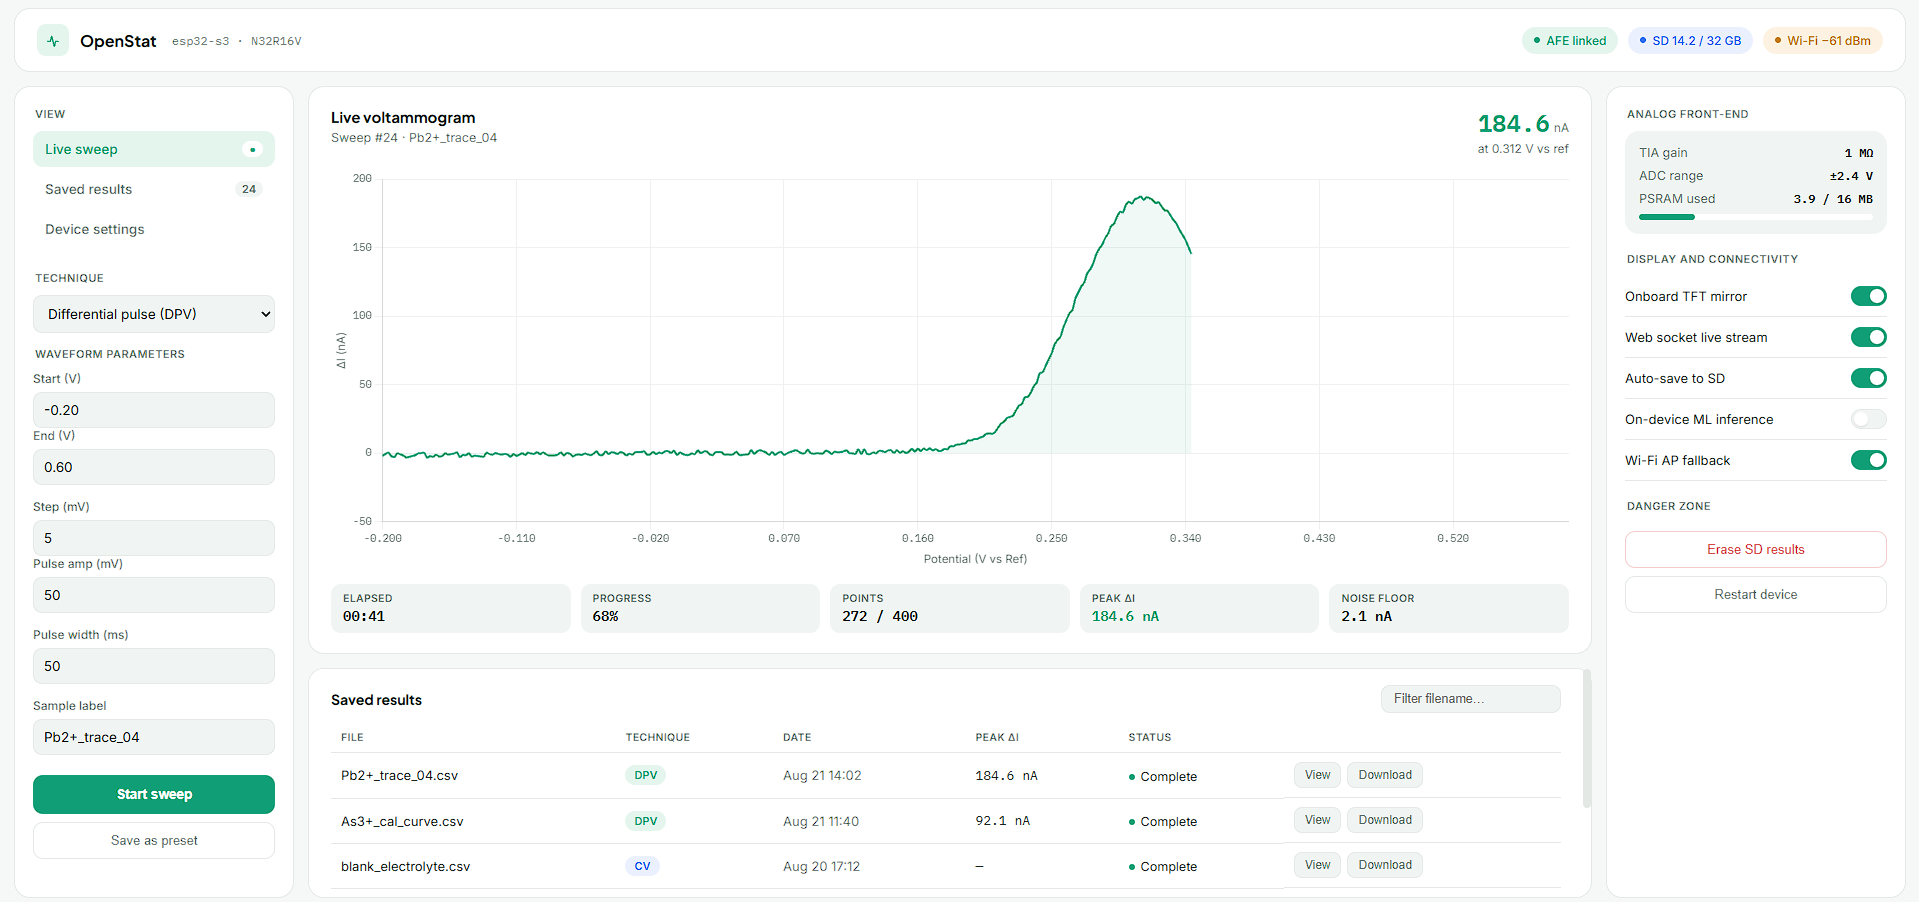
\includegraphics[width=0.7\linewidth]{figures/dashboard.png}
    \caption{The webserver dashboard for the potentiostat.}
    \label{fig:dashboard}
\end{figure}


\chapter{KiCad Schematic}
\label{app:kicad_schematic}
\begin{figure}[H]
    \centering
    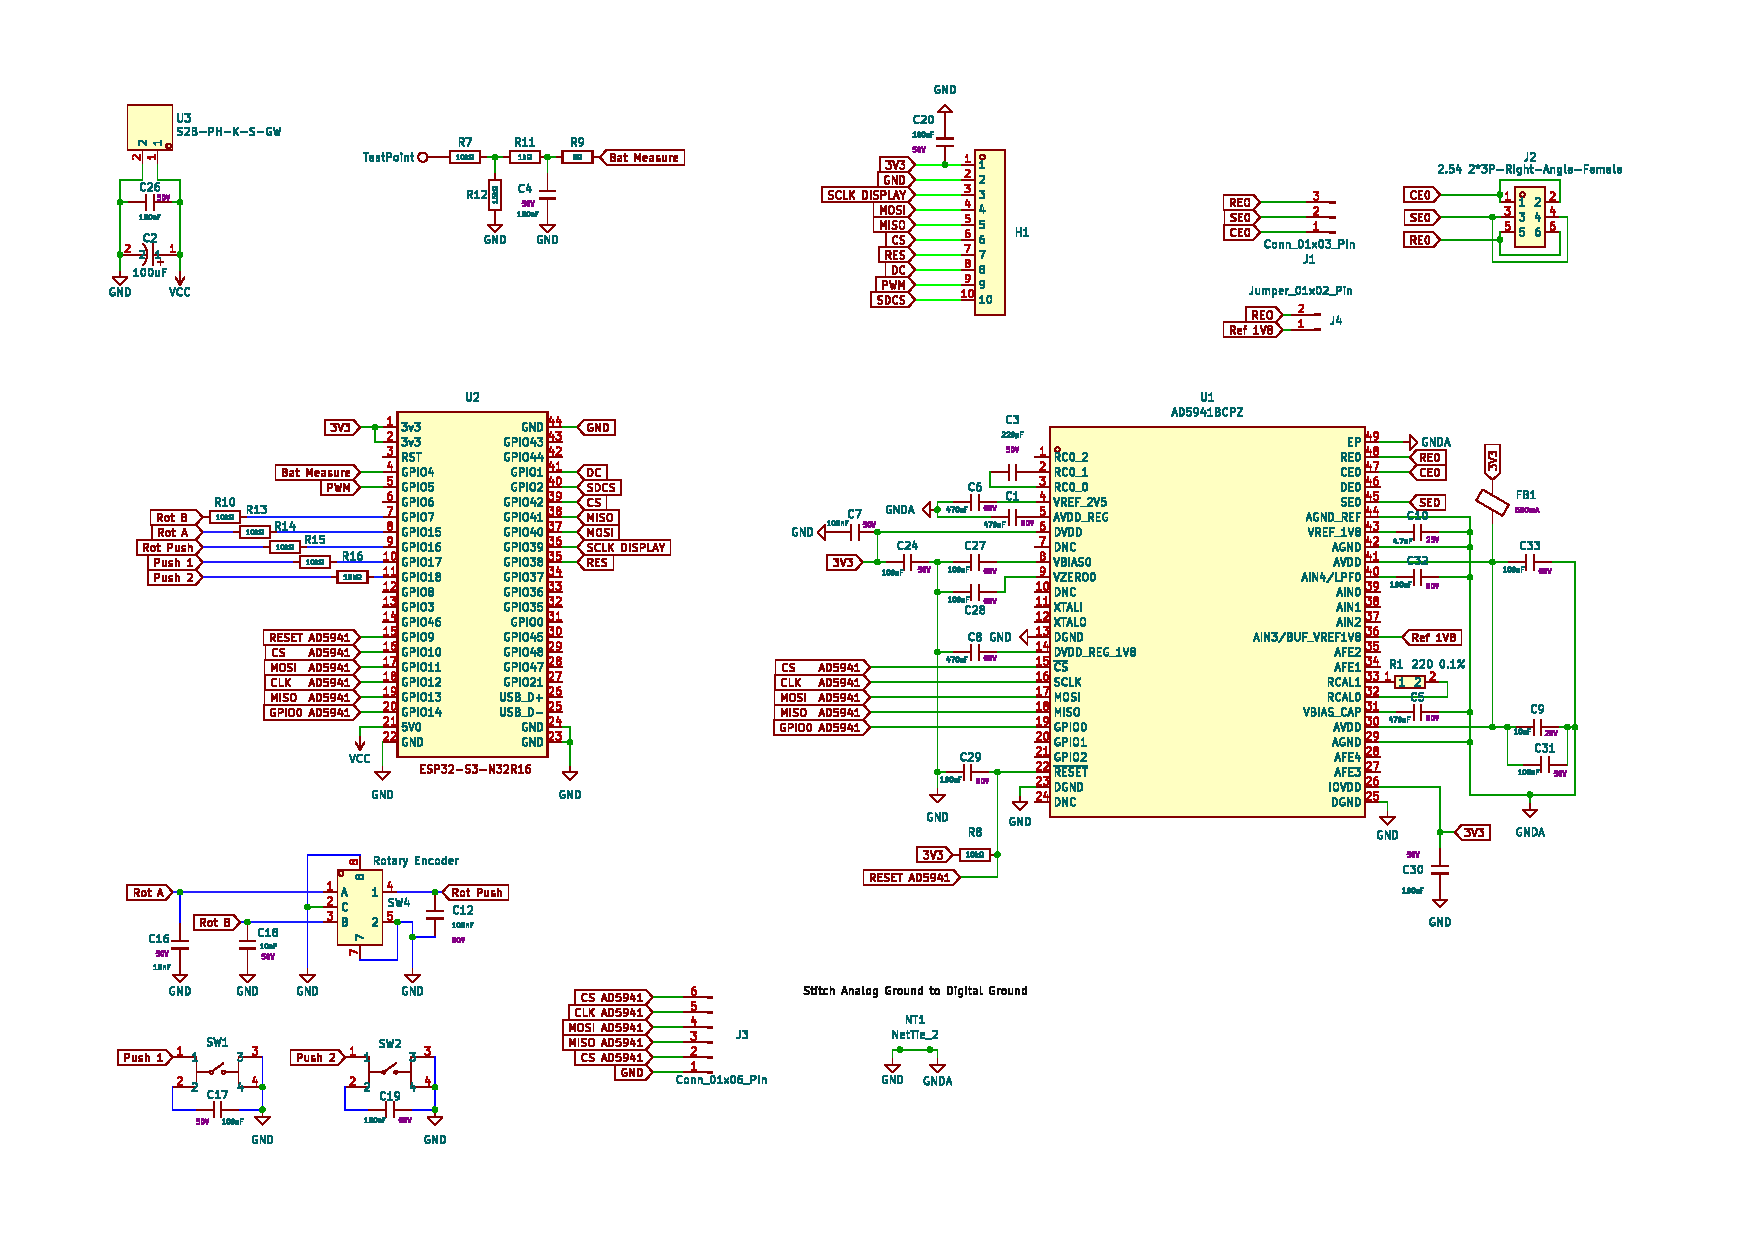
\includegraphics[angle=90, width=0.6\linewidth]{figures/KicadExport.pdf}
    \caption{The KiCad schematic for the potentiostat.}
    \label{fig:kicad_schematic}
\end{figure}

\chapter{KiCad PCB}
\label{app:kicad_pcb}
\begin{figure}[H]
    \centering
    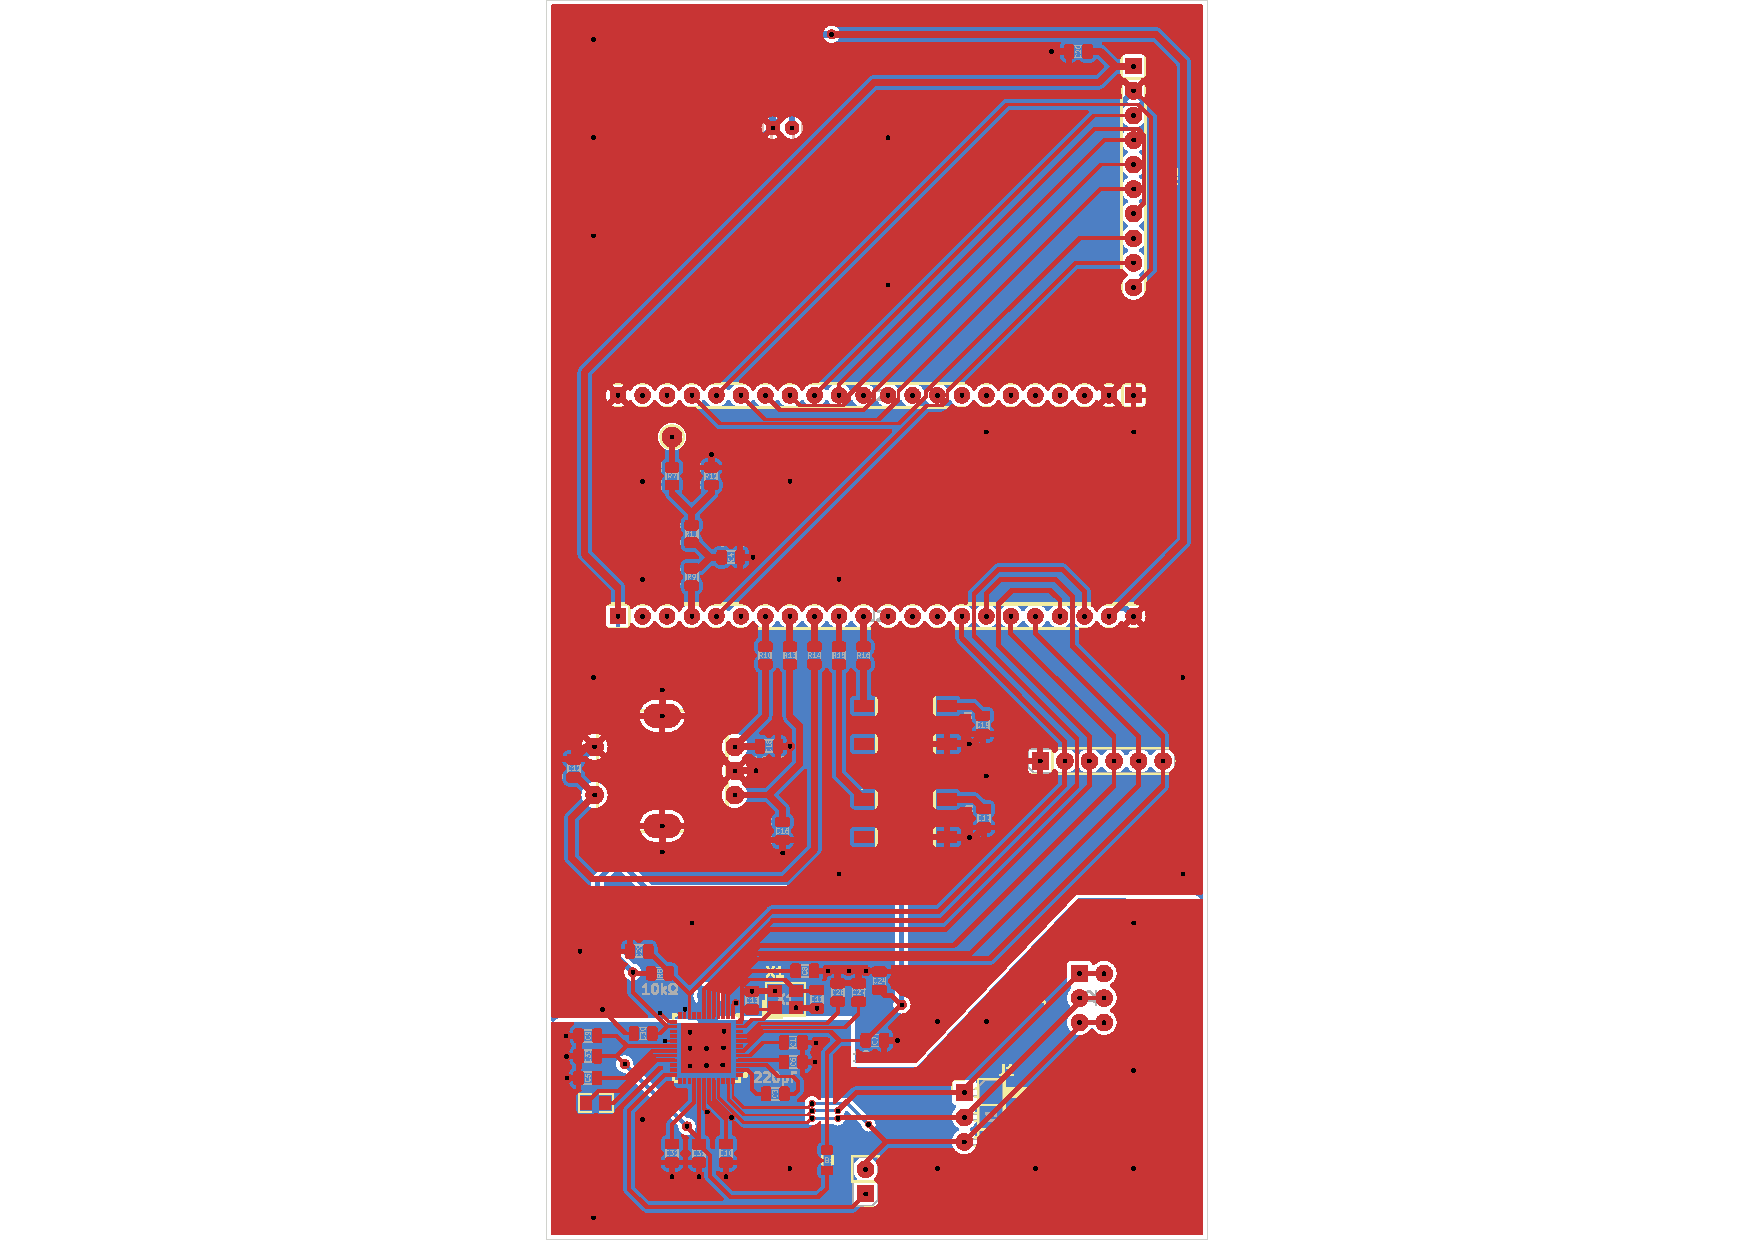
\includegraphics[angle=0, width=0.9\linewidth]{figures/pcbexport.pdf}
    \caption{The KiCad PCB for the potentiostat.}
    \label{fig:kicad_pcb}
\end{figure}


\chapter{Case Render}
\label{app:case_render}

\begin{figure}[H]
    \centering
    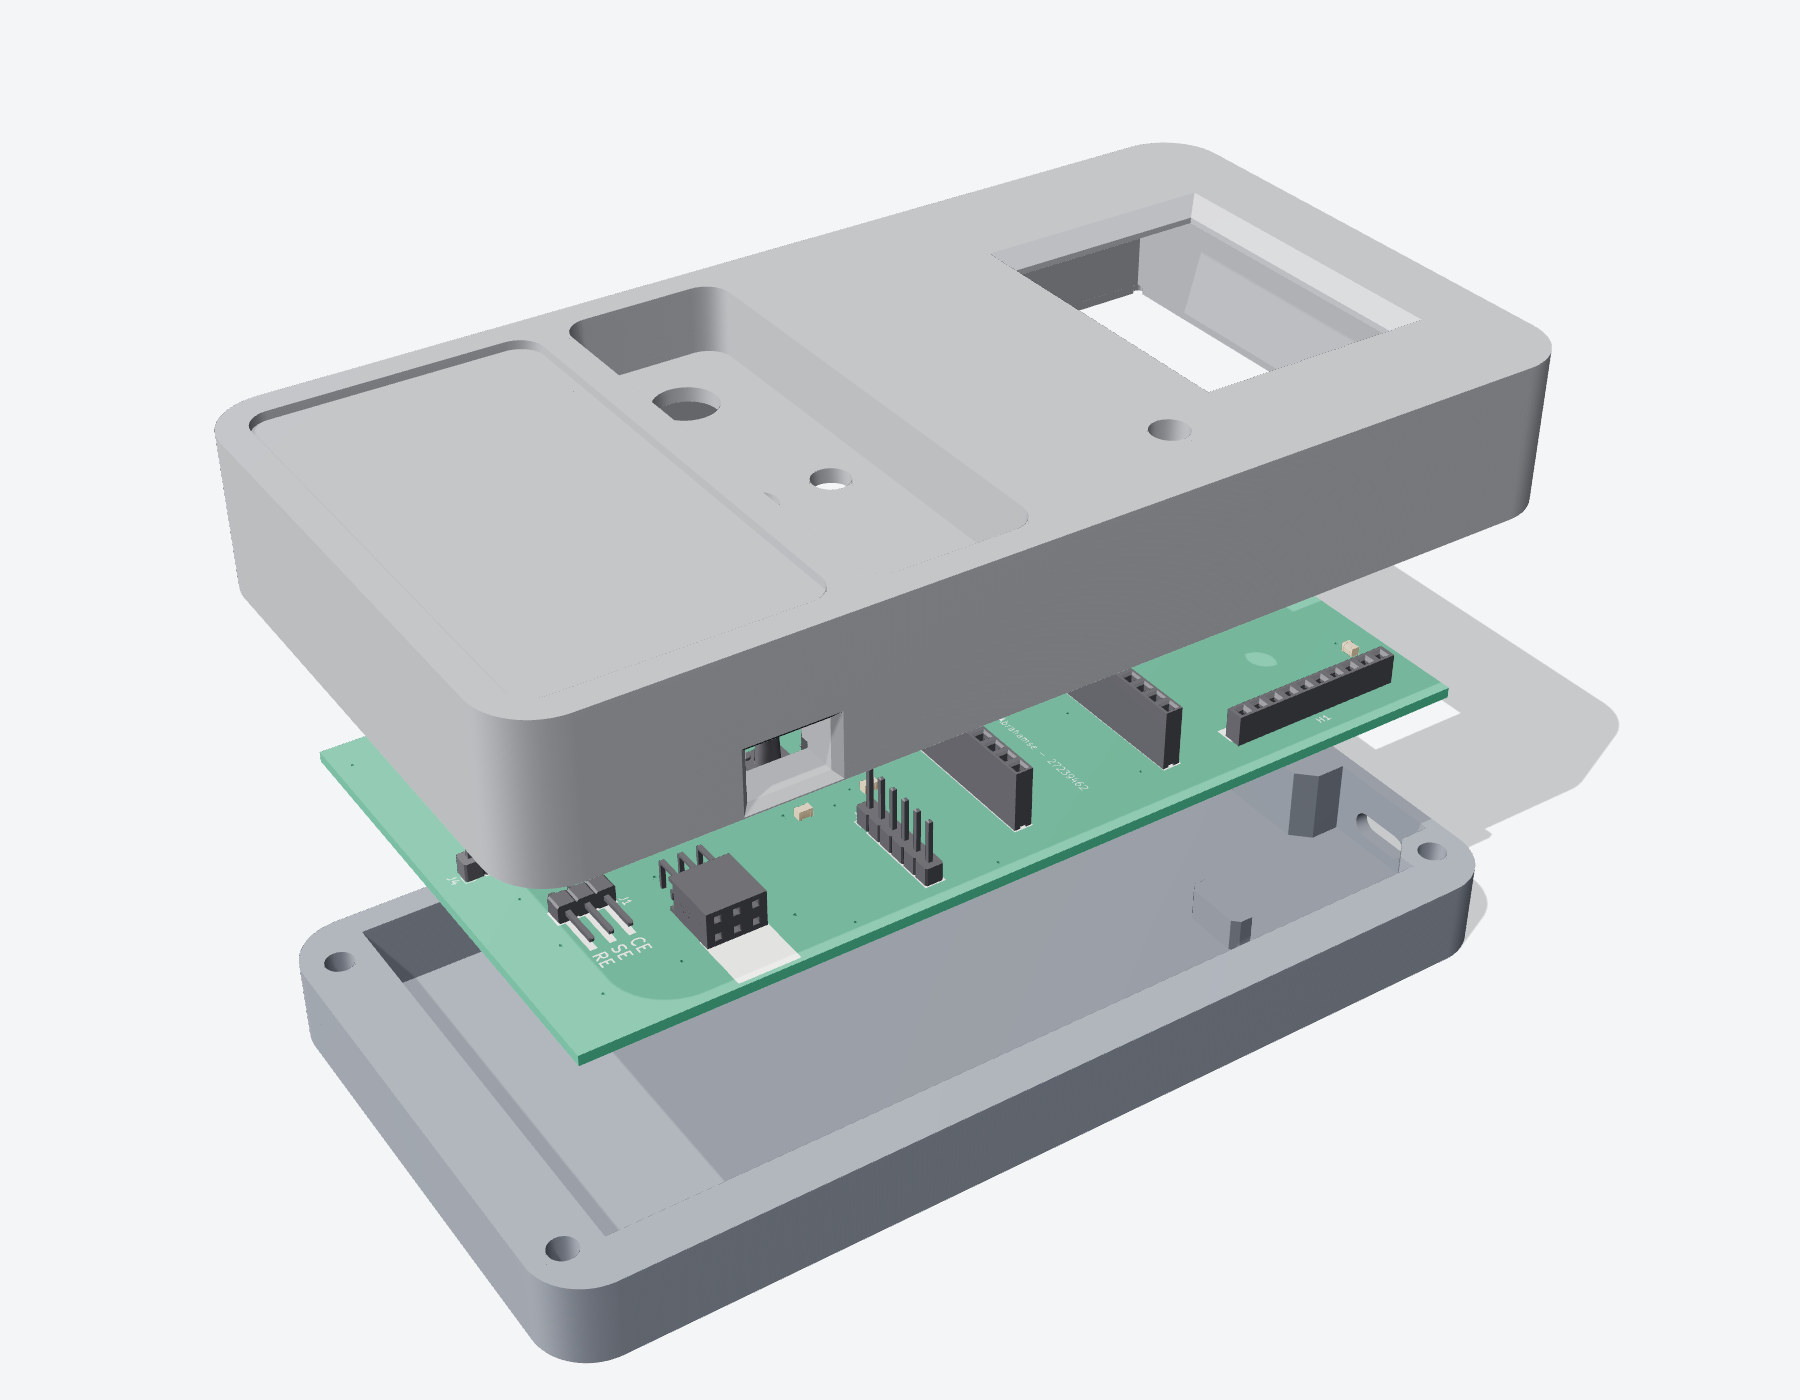
\includegraphics[width=0.7\linewidth]{figures/case model.png}
    \caption{The case render for the potentiostat.}
    \label{fig:case_render}
\end{figure}

\end{document}
